%%%%%%%%%%%%%%%%%%%%%%%%%%%%% Define Article %%%%%%%%%%%%%%%%%%%%%%%%%%%%%%%%%%
\documentclass[a4paper]{article}
%%%%%%%%%%%%%%%%%%%%%%%%%%%%%%%%%%%%%%%%%%%%%%%%%%%%%%%%%%%%%%%%%%%%%%%%%%%%%%%

%%%%%%%%%%%%%%%%%%%%%%%%%%%%% Using Packages %%%%%%%%%%%%%%%%%%%%%%%%%%%%%%%%%%
\usepackage{geometry}
\usepackage{graphicx}
\usepackage{amssymb}
\usepackage{amsmath}
\usepackage{amsthm}
\usepackage{booktabs}
\usepackage{lipsum}
\usepackage{graphicx}
\usepackage{color}
\usepackage{nth}
\usepackage{bm}
\usepackage{caption}
\usepackage{subcaption}
\usepackage{url}
\usepackage{array}
\usepackage{multirow}
%%%%%%%%%%%%%%%%%%%%%%%%%% Page Setting %%%%%%%%%%%%%%%%%%%%%%%%%%%%%%%%%%%%%%%
\geometry{a4paper}

%%%%%%%%%%%%%%%%%%%%%%%%%% Define some useful colors %%%%%%%%%%%%%%%%%%%%%%%%%%
\definecolor{ocre}{RGB}{243,102,25}
\definecolor{mygray}{RGB}{243,243,244}
\definecolor{deepGreen}{RGB}{26,111,0}
\definecolor{shallowGreen}{RGB}{235,255,255}
\definecolor{deepBlue}{RGB}{61,124,222}
\definecolor{shallowBlue}{RGB}{235,249,255}
%%%%%%%%%%%%%%%%%%%%%%%%%%%%%%%%%%%%%%%%%%%%%%%%%%%%%%%%%%%%%%%%%%%%%%%%%%%%%%%

%%%%%%%%%%%%%%%%%%%%%%%%%% Macros %%%%%%%%%%%%%%%%%%%%%%%%%%%%%%%%%%%%%%%%%%%%%
\DeclareMathOperator{\Lagr}{\mathcal{L}}
%%%%%%%%%%%%%%%%%%%%%%%%%%%%%%%%%%%%%%%%%%%%%%%%%%%%%%%%%%%%%%%%%%%%%%%%%%%%%%%


\begin{document}
  % custom title page
  \begin{titlepage}
  \begin{center}

    \vspace*{1cm}

    \textbf{\LARGE
    % Training and Deploying Computer Vision Models for Indoor Localisation
    % Exploring Deep Learning for Indoor Localisation: A Study on Room-Level Accuracy
    Navigating Indoors with Computer Vision: Exploring Deep Learning Approaches
    for Room-Level Indoor Localisation
    % Deep Learning for Accurate Room-Level Indoor Localisation: Feasibility and Evaluation
    % Enhancing Indoor Spatial Awareness: Deep Learning Approaches for Room-Level
    % Indoor Localisation
    }

    \vspace{1.5cm}

    % author
    \begin{minipage}[t]{5cm}
      \centering
      \textbf{Mika Senghaas} (Author) \\
      IT University of Copenhagen \\
      \textit{jsen@itu.dk}
    \end{minipage}
    \hspace{1cm}
    \begin{minipage}[t]{5cm}
      \centering
      \textbf{Stella Grasshof} (Supervisor) \\
      IT University of Copenhagen \\
      \textit{stgr@itu.dk}
    \end{minipage}

    \vfill

    % degree
    A Thesis presented for the Degree of \\
    \textbf{Bachelor of Science in Data Science}

    \vspace{0.8cm}

    
\includegraphics[width=0.4\textwidth]{figures/itu.jpg}

    \vspace{0.8cm}

    \textbf{IT University of Copenhagen}\\
    Computer Science Department\\
    \vspace{.5cm}
    May, 15th 2023

  \end{center}
\end{titlepage}

  \newpage

  % table of contents, list of tables, list of figures
  \tableofcontents
  % \listoftables
  % \listoffigures
  \newpage

  % Deep residual networks have emerged as a family of extremely deep
  % architectures showing compelling accuracy and nice convergence behaviors. In
  % this paper, we analyze the propagation formulations behind the residual
  % building blocks, which suggest that the forward and backward signals can be
  % directly propagated from one block to any other block, when using identity
  % mappings as the skip connections and after-addition activation. A series of
  % ablation experiments support the importance of these identity mappings. This
  % motivates us to propose a new residual unit, which makes training easier and
  % improves generalization. We report improved results using a 1001-layer ResNet
  % on CIFAR-10 (4.62% error) and CIFAR-100, and a 200-layer ResNet on ImageNet.
  % Code is available at: https://github.com/KaimingHe/resnet-1k-layers

  \begin{abstract} % (fold)
    \lipsum[1]
  \end{abstract}

  \section{Introduction}
  \label{sec:introduction}

  % outdoor localisation as solved problem 
  With the introduction of GPS (Global Positioning System), a satellite-based
  positioning system, localisation in outdoor spaces has become more efficient
  and accurate than ever before. Gradual commercialisation led to the technology
  rapidly transforming entire industries and personal navigation in every-day
  life. Today, outdoor localisation is widely considered a \textit{solved
  problem}.

  % gps struggles in indoor spaces
  The same cannot be said for indoor localisation. Because the transmitted radio
  signals sent out by the satellites in GPS systems are not strong enough to
  penetrate through walls and struggle with reflections from large buildings,
  the technology yields inaccurate results at best, and often becomes
  dysfunctional in indoor spaces.

  % indoor localisation techniques (broad overview)
  Finding alternative solutions to provide an accurate, cheap and robust indoor
  localisation systems has been a main focus of research in the past decades,
  and is becoming increasingly important in the light of the ongoing
  urbanisation of our living spaces and the emergence of autonomous robots and
  vehicles in our everyday life. Decades of research have led to the development
  of a variety of different indoor localisation technologies. Hardware-based
  systems use radio signals, transmitted by beacons, like Bluetooth, and
  Ultra-Wideband (UWB) or Wi-Fi, to localise an agent in a known environment.
  Software-based systems, like Simultaneous Localisation and Mapping (SLAM)
  algorithms, use sensors, like cameras or distance-measuring laser sensors, to
  localise an agent, while simultaneously creating a map of the environment.
  
  % short-comings of existing approaches
  While these approaches have proven to produce remarkable results, being
  capable of localising an agent with centimetre accuracy, they are limited for
  various reasons: Hardware-based system require an expensive initial setup,
  continuous maintenance of the signal-transmitting beacons, and are often not
  feasible in large environments. SLAM algorithms, on the other hand, require a
  meticulously handcrafted pipeline of feature detection, feature matching, and
  pose estimation that has to be fine-tuned by experts for each indoor space, to
  achieve outstanding results. All of the above short-comings of existing indoor
  localisation technologies make commercial applications rare and not unified in
  their approach. 

  % short-comings of existing approaches
  All of the above approaches work under the assumption that centimetre-accuracy
  is required for indoor localisation. However, this is not always the case. For
  some applications, like indoor navigation, it is sufficient to know the
  position of the agent with a meter or even room-accuracy, instead of
  centimetre accuracy. One example of such an application is the navigation in
  large indoor spaces, like airports, train stations, or shopping malls, where
  the goal is to guide the agent to a specific room or area. In these cases, the
  constraint of centimetre-accuracy can be relaxed, in favour of a simpler and
  more versatile solution.

  % success of deep learning in computer vision
  In the past decades, deep learning has proven to be a powerful tool in a
  wide-variety of tasks and has repeatedly proven remarkable capabilities in the
  field of computer vision. Amongst common task in computer vision is the task
  of image classification where the goal is to predict a label from a set of
  pre-defined labels.

  % deep learning for indoor localisation
  Motivated by the apparent lack of a simple, unified indoor localisation system
  and the success of deep learning in computer vision, this study investigates
  the applicability of modern deep learning techniques to the task of indoor
  localisation when viewing localisation as a classification task. The study
  presents the rigorous evaluation of several modern deep learning architectures
  on a challengingly small video dataset for mapping our a novel indoor space to
  imitate the real-world scenario of a new indoor space.

  % section introduction (end)

  \section{Background} % (fold)
  \label{sec:background}

  Producing accurate, robust and cheap localisation systems is not a novel task,
  but has been a focus of research at the intersection of robotics, computer
  vision and machine learning for decades. A wide variety of approaches using
  different sensory information, assuming different agent and environment
  set-ups have been proposed.

  \subsection{Hardware-Based Indoor Localisation} % (fold)
  \label{sub:hardware-based-indoor-localisation}

  The approach conceptually closest to GPS-based outdoor localisation systems
  are hardware-based indoor localisation systems. Because radio signals
  transmitted by satellites are incapable of penetrating through walls, various
  close-proximity radio signals have been proposed to be used for indoor
  localisation, such as Bluetooth~\cite{bluetooth1, bluetooth2}, Ultra-Wideband
  (UWB)~\cite{uwb1, uwb2} or Wi-Fi~\cite{survey1, survey2}.

  No matter the radio signals, three main approaches can be distinguished:
  (1) Angle of Arrival (AOA), (2) Time of Arrival (TOA) and (3)
  RSSI-Fingerprinting (RSSI-FP)~\cite{survey2}. 

  In AOA approaches, transmitting beacons, called access points (APs), are
  measuring the distance and angle between a beacon and an agent. The
  intersection between the lines of sight (LoS) of at least three APs yields
  the position of the agent. 

  TOA approaches (such as GPS) use the received signal strength (RSS) to
  estimate the distance between an agent and the AP through a propagation model.
  Given the distance estimates of at least four APs, the agent's position can be
  determined by an approach called tlateration, which is based on the idea
  that an agent's position in three-dimensional space can be uniquely determined
  by the intersection of four spheres with known radius and centres. Clearly,
  TOA approaches require knowledge about the position of the APs, which makes
  them less practical in indoor spaces, where the position of the APs is often
  unknown.

  The approach with the most recent research interest is RSSI-FP. It can be divided into
  two separate phases: In an offline mapping phase, the indoor environment is
  mapped by repeatedly measuring the RSSI values of the APs at various reference
  points (RPs). A vector of RSSI values then uniquely identifies each RP and is
  stored in a database. In the online localisation phase, the agent's position
  is then determined by dynamically comparing the agent's RSSI vector against
  the RSSI vectors of the RPs stored in the database. Ultimately, the agent's
  position is determined as the position of the RP with the most similar RSSI
  vector according to some similarity metric. While this approach alleviates the
  need for the precise positions of the APs, it requires a time-intensive
  offline mapping phase and is sensitive to changes in the environment.

  Many of the proposed technologies assume massive infrastructure deployments
  and incur high setup and maintenance costs. Wi-Fi based approaches seem most
  promising, given their ubiquitous availability in modern indoor spaces. 
  However, all hardware-based approaches suffer measurements errors that
  underlie the triangulation (AOA), multilateration (TOA) or similarity metric
  (RSSI-FP) approaches. Such errors are caused by reflections (multipath
  effect), blockage (shadowing), and signal attenuation (fading).

  % challenge: incurs costly initial setup and maintanance challenge: distorted
  % rssi scans because of multipath effect, shadowing, fading, and delay
  % distortion

  % subsection hardware_based_indoor_localisation (end)k

  \subsection{Simultaneous Location and Mapping (SLAM)} % (fold)

  % SLAM
  Amongst the most promising approaches are SLAM (Simultaneous Localisation and
  Mapping) algorithms. SLAM algorithms aim to localise an agent inside an
  unknown environment, while simultaneously building a consistent map of the
  environment. There exist a variety of different approaches to SLAM, depending
  on the type of sensors that are used. For example, Visual SLAM (V-SLAM)
  algorithms use camera input, and LidarSLAM algorithms use distance-measuring
  laser sensors. 

  Most related to this study are monocular V-SLAM algorithms, because they use a
  single camera to estimate the position of the agent. The very first monocular
  feature-based V-SLAM algorithms, MonoSLAM, was proposed in
  2007~\cite{mono-slam}. The research is considered a break-through in V-SLAM
  algorithms, as it is considered the first algorithm producing accurate results
  while only using a single camera. Previously, V-SLAM algorithms required
  multiple cameras or other sensors to overcome the problem of depth estimation
  using a single camera.

  Since then, many adjustments and optimisation have been proposed to the
  algorithm to make it more robust and accurate. Typically, the adjustments
  replace or modify one of the components of the pipeline. For example, the
  ORB-SLAM~\cite{orb-slam} algorithm uses a bag-of-words approach for feature
  matching, and the PTAM~\cite{ptam} algorithm uses a parallel computing, which
  was shown to improve the accuracy of the algorithm. In recent years, such
  modifications are often based on deep learning techniques to improve on
  sub-parts of the SLAM pipeline. For example, the DeepVO~\cite{deep-vo}
  algorithm uses a convolutional neural network to estimate the camera pose from
  a sequence of images. 

  Overall, SLAM algorithms have shown impressive results and are in commercial
  use in many applications. However, they are still not robust enough to be
  deployed in safety-critical applications, such as autonomous driving. The

  \subsection{Deep Learning in Computer Vision} % (fold)

  Computer vision is one of the major subfields of artificial intelligence and
  is concerned with the automatic extraction of information from images. The
  extraction of information from images is a challenging task, because images
  are high-dimensional and unstructured. This makes it a challenging environment
  for hand-crafted algorithms, which are often based on heuristics and
  assumptions about the data. For this reason, deep learning techniques have
  been applied successfully to many computer vision tasks, and dominate the
  benchmarks of most computer vision tasks.

  Arguably the offset of the deep learning wave in computer vision was the
  success of the AlexNet~\cite{alexnet} architecture in the 2012 ImageNet Large
  Scale Visual Recognition Challenge~\cite{imagenet}, which crushed the
  competition by increasing the Top-5 Accuracy from 73.8\% to 84.7\%. At the
  time, the dominating approach to computer vision tasks was based on
  hand-crafted features, such as SIFT~\cite{sift} and HOG~\cite{hog}. AlexNet
  was the first successful adaption of a deep convolutional neural network
  (CNN), which were first proposed by LeCun et al.~\cite{lenet} in 1998. 

  In the following years, CNN-based architectures with increasing depth and
  width, and architectural improvements, such as weight initialisation, batch
  normalisation, residual connections~\cite{vgg, google-lenet, resnet, xception} were
  proposed and pushed the state-of-the-art further. The introduction of ResNet
  in 2015 is considered a cornerstone in convolutional neural networks
  architectures, as it allowed for the training of much deeper networks without
  the problem of vanishing gradients. In 2017, the Xception~\cite{xception}
  architecture was proposed, which is based on the Inception architecture, but
  uses depth-wise separable convolutions.

  With the success of Transformer-based architectures for language modelling in
  natural language processing~\cite{transformer}, the computer vision community
  was quick to adapt the architecture to computer vision tasks. The first
  successful application of the Transformer architecture to computer vision was
  the Vision Transformer (ViT)~\cite{vit}, which achieved state-of-the-art on
  many image classification benchmarks~\cite{cifar-10, cifar-100, imagenet}.

  Beyond image classification, the task of video classification has recently
  gained traction with the introduction of large-scale video datasets, such as
  Kinetics~\cite{kinetics}, more computational resources and an increasing need
  to understand video data in our multi-media world. Continuously predicting on
  a stream of frames is clearly related to image classification, but adds
  complexity to the task, because of the temporal dimension and increase in data
  size. Video Classification can be solved by combining CNNs with recurrent
  neural networks (RNNs) or by using 3D convolutions. The first approach by
  Donahue et. al proposes long-term recurrent convolutional networks (LRCNs),
  which use a CNN to extract features from each frame, which are then fed into a
  LSTM~\cite{lrcn} to produce a sequence of predictions. Alternative approaches
  use 3D convolutions to capture the spatio-temporal nature of video
  data~\cite{c3d, i3d}. Yet another approach, called SlowFast~\cite{slowfast}
  uses two separate CNN networks to capture spatial and temporal information
  separately, which are then combined in the final layers of the network.

  % subsection deep-learning (end)

  % section background (end)

  \section{Data} % (fold)
  \label{sec:data}

  Framing the problem of indoor localisation as a classification task requires a
  labelled data set, which consists of sequentially-arranged pairs of video
  frames and location labels. A single video clip $C$ consists of a sequence of
  $n$ frames $x_0, ..., x_n$ and a sequence of $n$ location labels $y_0, ...,
  y_n$, where the $i$-th pair of the sequence is the tuple $(x_i,y_i)$ and
  denotes the location at a specific frame. A single frame $x_i$ is a RGB image,
  represented as a three-dimensional tensor of shape $3 \times H \times W$,
  where $H$ and $W$ are the height and width of the image, respectively. A
  single location label $y_i$ is a scalar value, which identifies the location
  of the agent at the time of the frame. 

  \subsection{Data Collection} % (fold)
  \label{sub:data-collection}

  % place of data collection
  The data set was collected from a single camera of a mobile
  device~\footnote{iPhone 11 Pro recording at 30 FPS with 2426x1125 HD
  resolution} that was hand-held by a human agent while walking around an indoor
  building. The chosen location for the data collection was the main building of
  the Southern Campus of the Copenhagen University (Danish: K\o{}benhavns
  Universitet, KU) in Copenhagen S, Denmark. The building is a large
  multi-storey building with a total of six floors, and is used for teaching and
  research purposes. The location was deemed compatible with this study, as it
  both has distinctive indoor features (e.g. coloured walls, unique structures,
  etc.), but also poses a challenge for the model, for example, due to the
  similarity of the floor plan across floors. For the scope of this project, the
  data collection was limited to the first two floors. The publicly accessible
  areas were separated into 21 different location labels, which are shown in Figure~\ref{fig:map}.
  Whenever possible, the location labels were designed in close correspondence
  to the building's official floor plan, but given more descriptive names.

  % figure
  \begin{figure}[ht]
    \centering
    % subfigure
    \begin{subfigure}[b]{.9\linewidth}
      \centering
      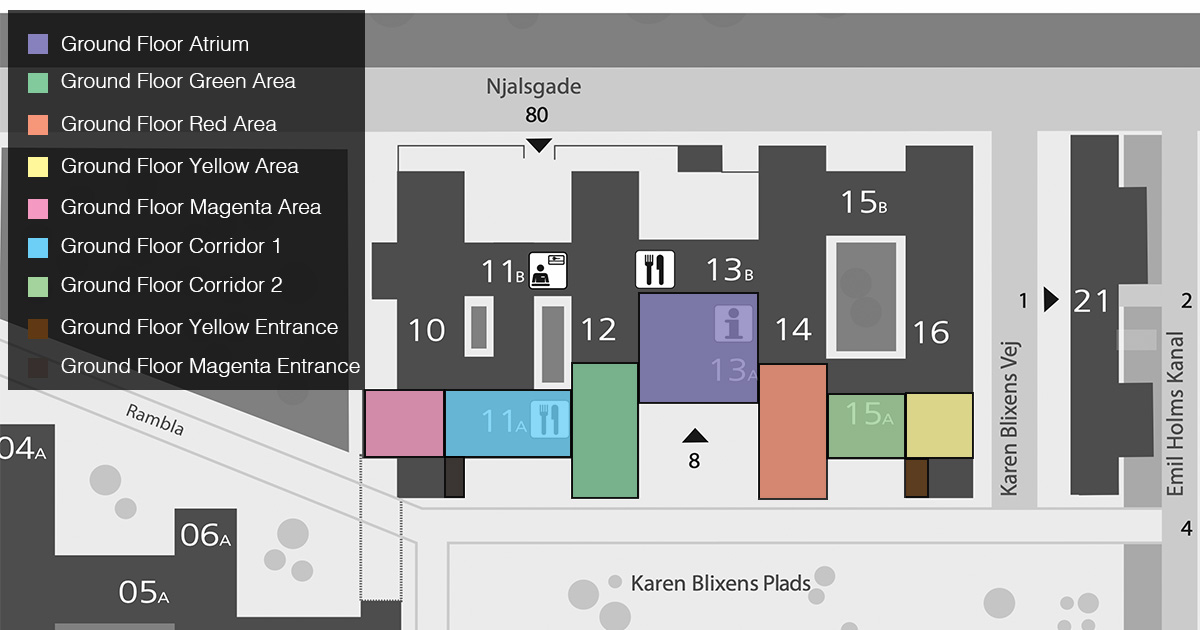
\includegraphics[width=\linewidth]{figures/map-ground-floor.jpg}
      \caption{Ground Floor}
      \label{fig:map-ground-floor}
    \end{subfigure}
    \hfill
    % subfigure
    \begin{subfigure}[b]{0.9\linewidth}
      \centering
      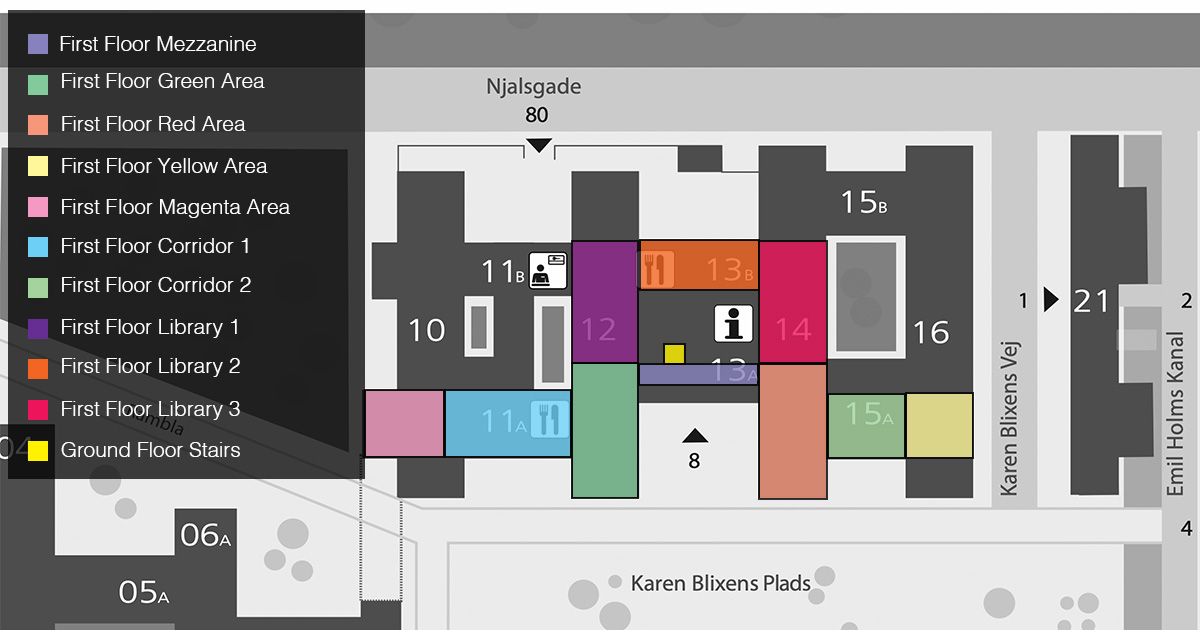
\includegraphics[width=\linewidth]{figures/map-first-floor.jpg}
      \caption{First Floor}
      \label{fig:map-first-floor}
    \end{subfigure}
    \caption{Map of KU Southern Campus Main Building with Location Labels}
    \label{fig:map}
  \end{figure}

  
  % statistics of the data
  A total of 53 video clips were recorded, with an average duration of $\sim 57$s,
  amounting to a total number of $\sim 50$ minutes of footage. Out of the total
  53 video clips that were recorded, 37 were used for training and 16 were used
  for validation. Table~\ref{tab:data-stats} shows more statistics of the raw
  data in the two different splits.

  \begin{table}[ht]
    \centering
    \begin{tabular}{llll}
    \toprule
    \bfseries Split & Total Clips & Total Seconds & Total Minutes \\
    \midrule
    Training & 37 &  2240 & 37 \\
    Testing & 16 & 783 & 13 \\
    \bottomrule
    \end{tabular}
    \caption{Statistics of the Raw Data in Training and Testing Splits}
    \label{tab:data-stats}
  \end{table}

  % time of data collection
  An ideal model learns robust indoor features that are invariant to natural 
  variations in the indoor space from training data collected in a minimal time
  span, as this minimises the initial cost and effort for data collection.
  To evaluate the model's robustness towards these variations, a different
  philosophy was adopted for the collection of training and testing data.

  While the 37 training clips were recorded on just two days, the 16 testing
  clips were recorded on four different days, two to four weeks after the
  initial training data collection. This was done to make the testing data
  closer resemble real-world scenarios, and thereby make the testing metrics
  more robust.
  
  % TODO: figure about the time of data collection (side-by-side, one where hue
  %       denotes the split and the other where hue denotes the clips per day)

  % subsection data-collection (end)

  \subsection{Data Annotation} % (fold)
  \label{sub:data-annotation}
  
  % subsection subsection name (end)
  To match the location labels to the video footage, each clip $C$ was manually
  annotated by denoting the starting and ending time stamps of a location label.
  The information was stored in a standardised format and later used in the
  pre-processing of clips into frame-location pairs.
  

  \subsection{Data Preprocessing} % (fold)
  \label{sub:data-preprocessing}

  The raw video clips and manual annotation of location labels, had to be
  pre-processed before they could be used for training deep learning models.

  The video footage was resized to a resolution of 224x224 pixels, which is the
  input resolution of most modern foundation models for image and video
  classification, which were used in this project. Furthermore, it decreases the 
  total data amount significantly, which allowed for less disk usage and faster
  loads into memory during training.

  Next, instead of extracting all 30 frames per second, the video footage was
  downsampled to a much lower frame rate of 1 FPS. This was done to reduce the
  total data amount, and to reduce over-fitting of the model to the training
  data. It was hypothesised, that because of the strong local dependency of
  consecutive frames, consecutive frames are highly correlated, thus including
  such frames does not introduce any additional variance, but redundancies that
  are harmful for the model's generalisation ability. Empirical experiments
  confirmed that downsampling indeed reduces over-fitting, and was therefore
  adopted across all experiments.

  Finally, the pre-processed video footage was aligned with the manual location
  labels by extracting a frame per second from the video and matching it against
  the location label that was active at that time. After pre-preprocessing,
  there exist pairs $(x_i, y_i)$, where $x_i$ is pre-processed, extracted frame
  of size 224x224 pixels, and $y_i$ is the corresponding location identifier.
  The frames were stored in a way that allowed for easily sampling both a random
  frame-location pair $(x_i, y_i)$ for image classification models, or a
  sequence of consecutive $n$ frames from a clip $([x_0, \ldots, x_n], [y_i,
  \ldots y_n])$ for video classification models. Here the sequence of frames was
  represented as a 4D-tensor of size $n \times 3 \times 224 \times 224$.

  Figure~\ref{fig:preprocessed-data} shows $n=4$ consecutive frame-location
  label pairs after preprocessing. As can be seen, even at a frame rate of 1
  FPS, neighbouring frames are still similar to each other. Further, the
  annotation at the transition from one location to another was often difficult
  to determine, as one could annotate strictly according to the device position
  or the view of the camera. This likely resulted in some frames being annotated
  with the wrong location label.

  % figure
  \begin{figure}[ht]
    \centering
    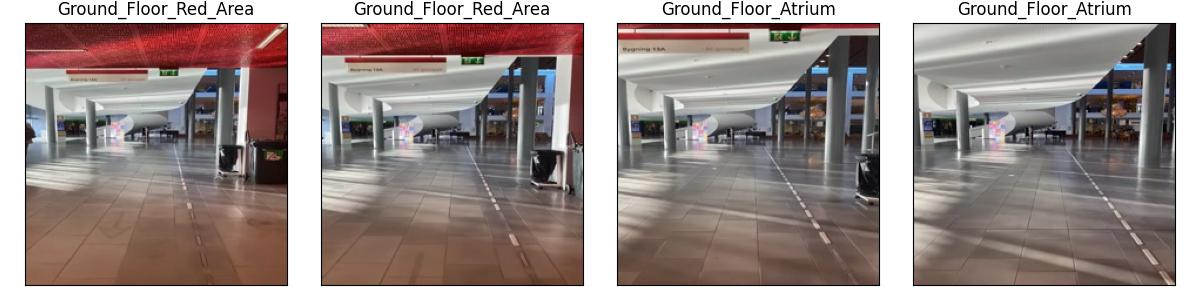
\includegraphics[width=\linewidth]{figures/data-example-batch.jpg}
    \caption{Examples of preprocessed frame-location pairs}
    \label{fig:preprocessed-data}
  \end{figure}

  % TODO: frame preprocessing: tofloat(), normalisation, standardisation
  
  % subsection data-preprocessing (end)
  
  % section section name (end)

  \section{Methodology} % (fold)
  \label{sec:methodology}


  \subsection{Models} % (fold)
  \label{sub:models}

  A deep learning model is supposed to learn a function $f: X \rightarrow Y$,
  where $X$ represents the input space and $Y$ the output space. By having
  framed the task of indoor localisation as a classification problem, the output
  space is the discrete set of location labels, $Y = \{l_1, \ldots, l_n\}$.
  Two approaches are viable for the input space $X$:

  \begin{enumerate}

    \item \textbf{Image Classification}: The input space $X$ is a single frame,
      $(3, H, W)$ and the output space is a single location label $y \in Y$.
      The model treats consecutive frames independently, and
      therefore disregards the temporal dimension of the video.

    \item \textbf{Video Classification}: The input space $X$ is a sequence of
      $N$ frames, $(x_1, \ldots, x_n)$, and the output space $Y$ is a sequence
      of $N$ location labels, $(y_0, \ldots, y_n)$, where each $y_i \in Y$. The
      model considers the temporal dimension of the video, and learns to
      classify the location label of a sequence of frames. In reality, the input
      sequence has a maximum context length $K$, meaning that the model
      continuously predicts on the previous $K$ frames.

  \end{enumerate}

  % explain that what CNN architecture is 
  % explain that what RNN architecture is
  % dominate computer vision tasks and are therefore used here
  % introduce notion of cnn module (any module that takes a single frame and
  % outputs a high-level feature representation) and rnn module (any module that
  % is capable of taking a sequence of frames and outputs a high-level feature
  % representation for each of them)

  % explain why video classifiers and transformers are disregarded

  \begin{figure}[ht]
    \centering
    \begin{subfigure}[b]{0.42\linewidth}
      \centering
      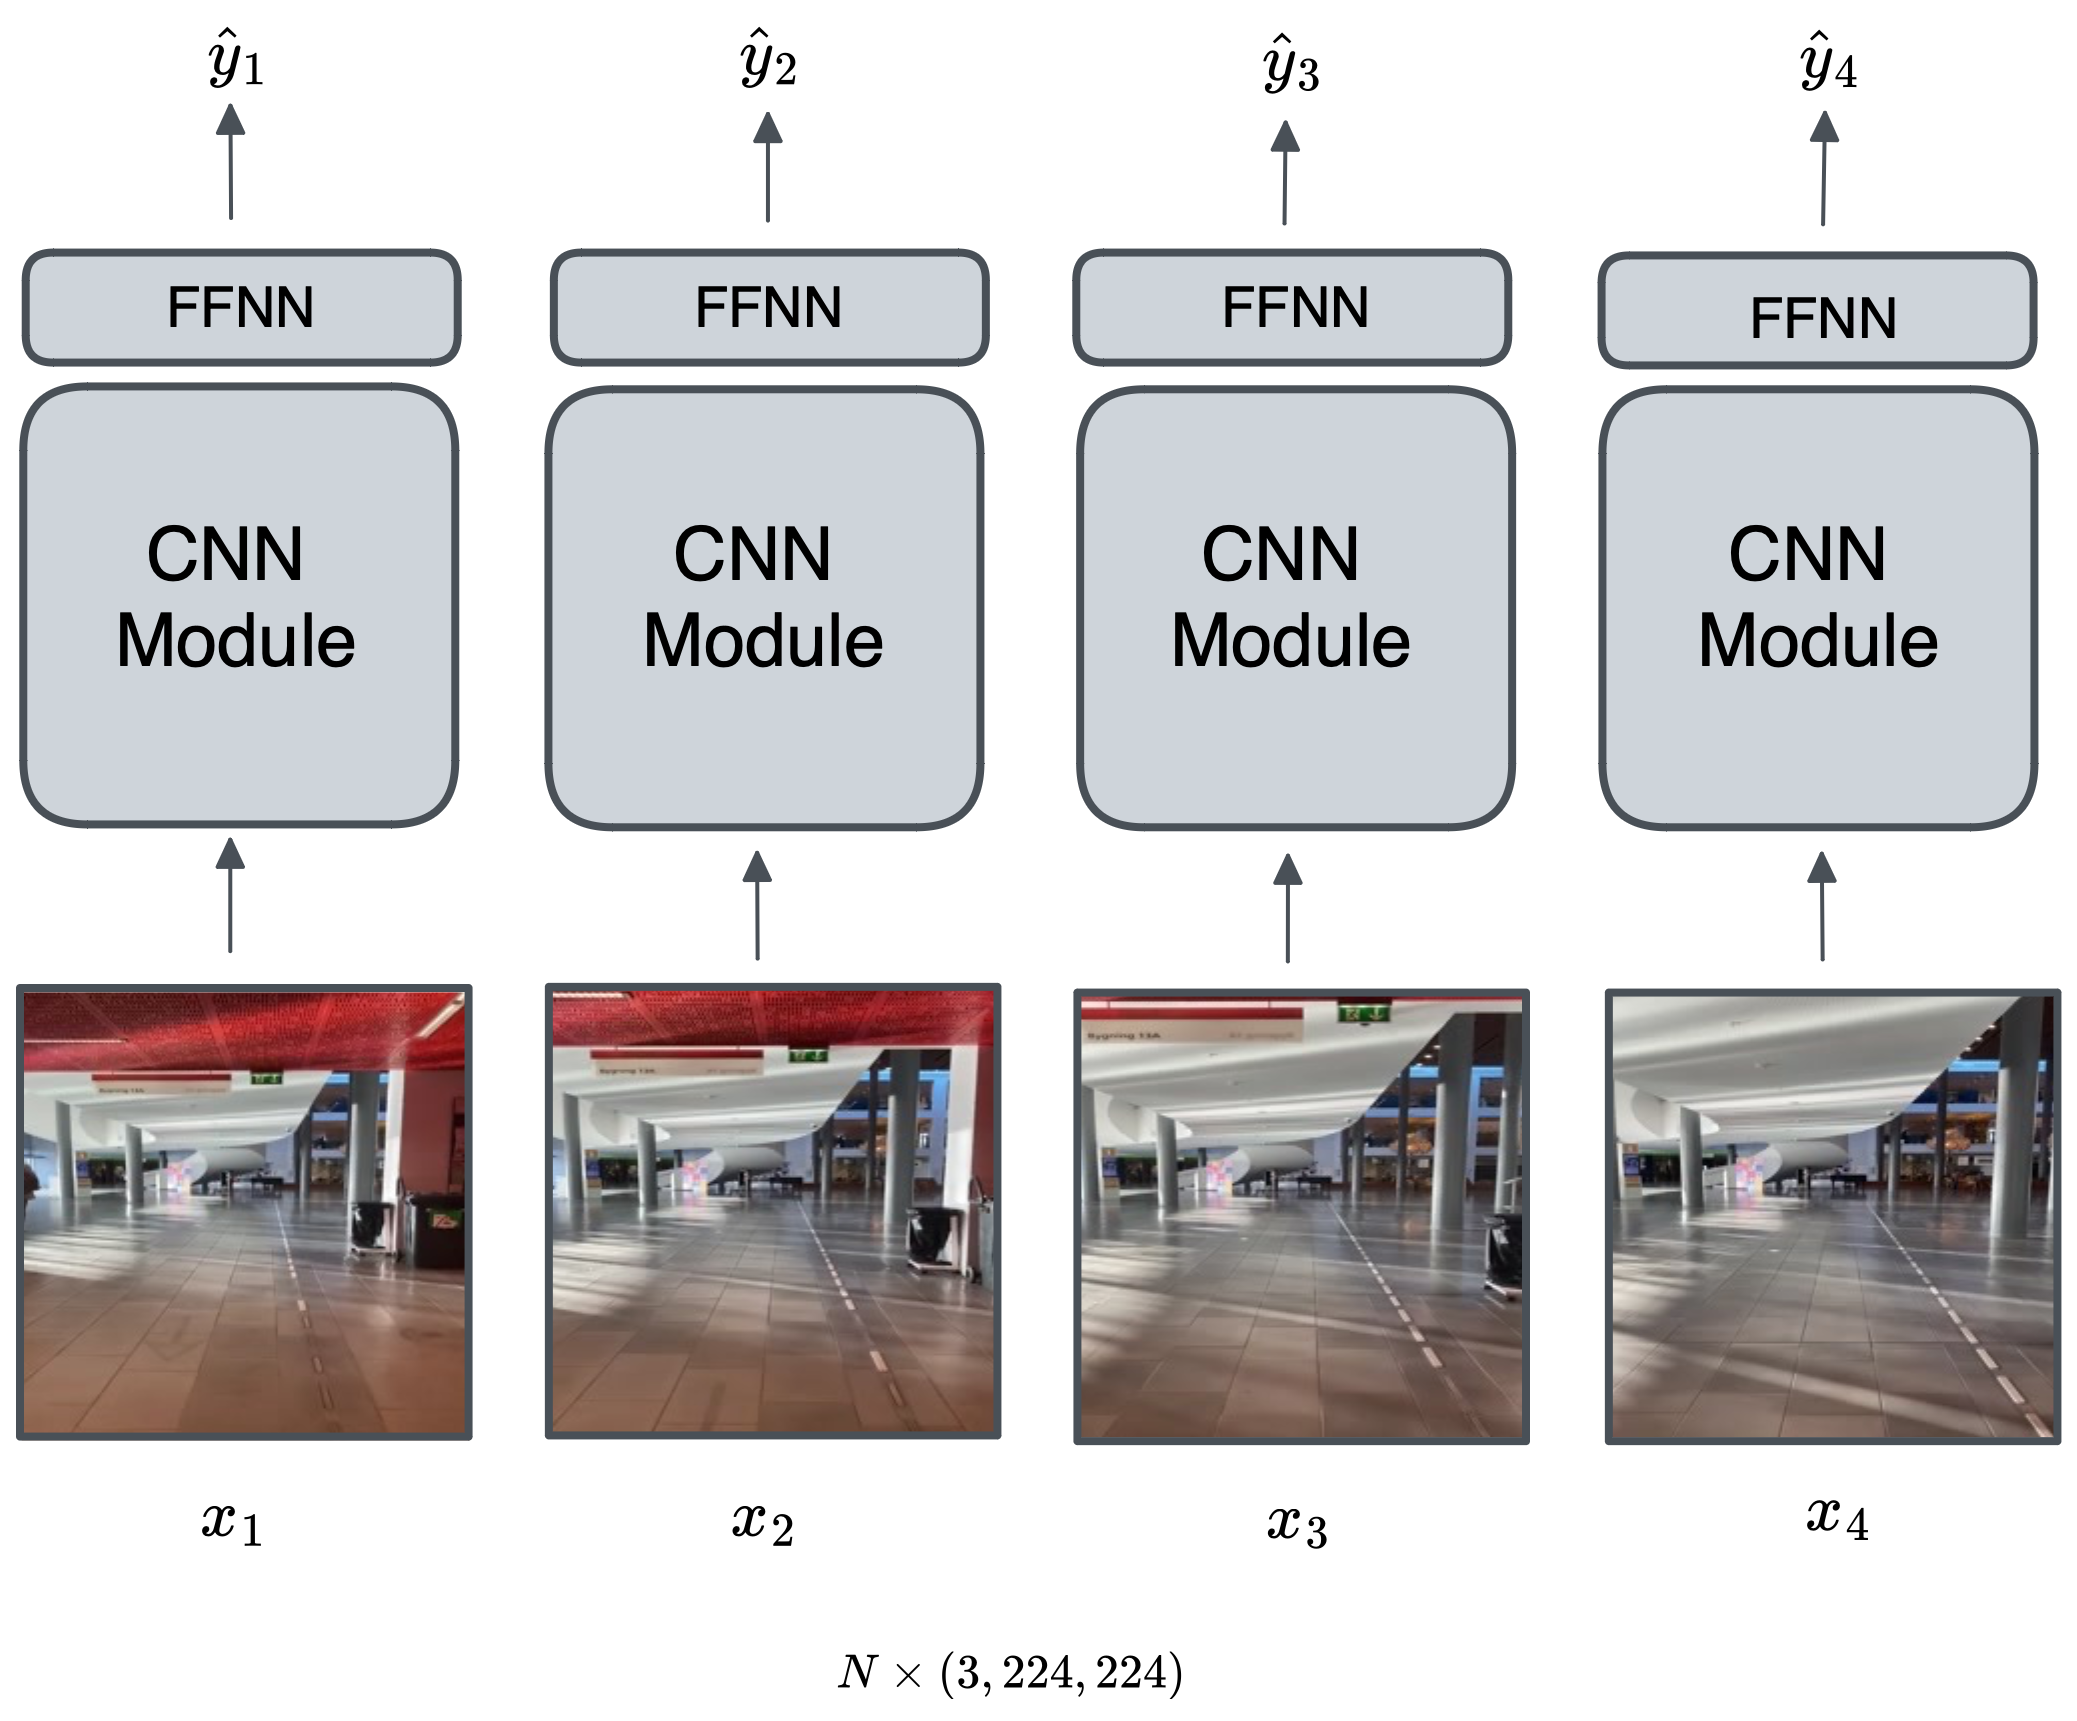
\includegraphics[width=\linewidth]{figures/cnn-architecture.png}
      \caption{Image Classification Architecture}
      \label{fig:cnn-architecture}
    \end{subfigure}
    \hfill
    \begin{subfigure}[b]{0.42\linewidth}
      \centering
      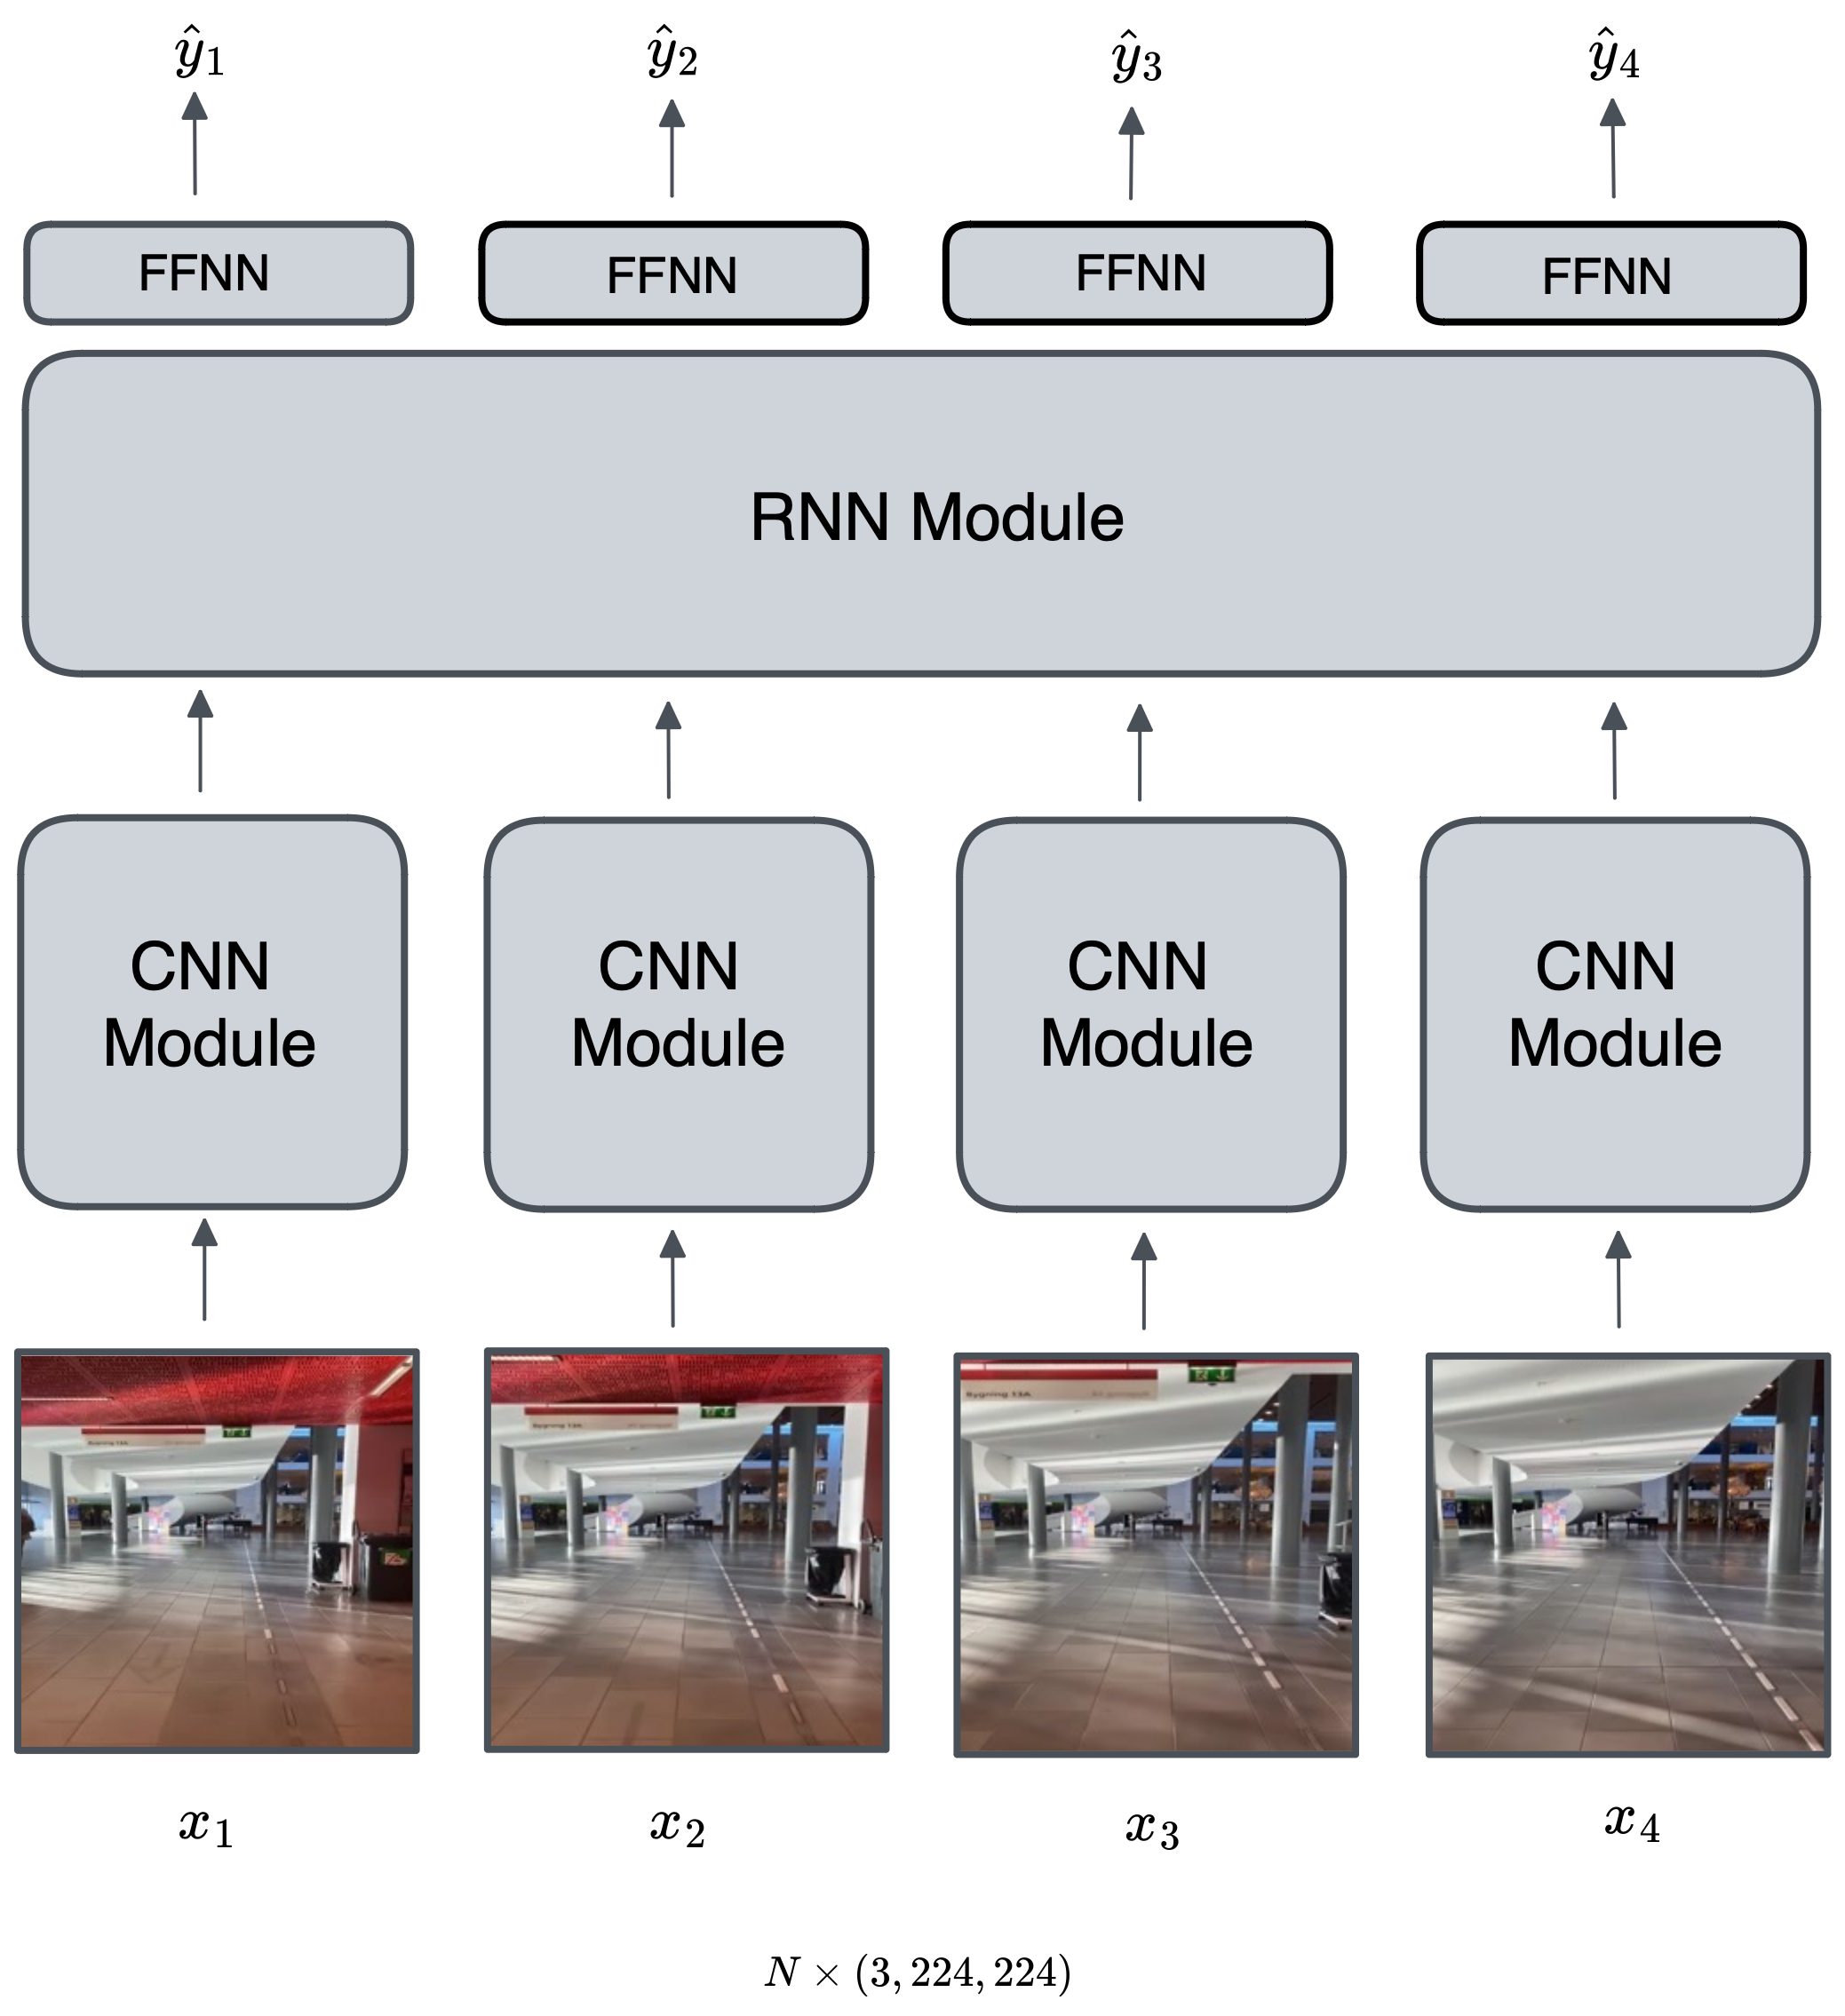
\includegraphics[width=\linewidth]{figures/rnn-architecture.png}
      \caption{Video Classification Architecture}
      \label{fig:rnn-architecture}
    \end{subfigure}
    \caption{Model Architectures}
    \label{fig:model-architectures}
  \end{figure}

  Figure~\ref{fig:model-architectures} shows the high-level architecture of the two
  approaches. For an image classification model, a sequence of $N$ (here $N=4$)
  frames are independently fed into a convolutional neural network (CNN), which
  outputs a feature vector for each frame. CNNs are a class of deep neural
  networks that are applied to analyse visual imagery. They are composed of
  several layers of alternating convolutional and pooling filters, which are
  applied to the input image to extract high-level feature representations.
  These high-level feature representations are then fed into a fully connected
  neural network (FCNN), which outputs a probability distribution over the
  location labels.

  For a video classification model, all $N$ consecutive frames are independently
  passed through a CNN module. The sequence of high-level feature
  representations is then fed into a recurrent neural network (RNN), which
  outputs a probability distribution over the location labels for each frame by
  placing a fully connected layer (classification head) to the output vector
  associated to each frame in the RNN module. A recurrent neural network (RNN)
  is a class of deep neural networks that is applied to analyse sequential data.
  Although they are mostly applied to natural language processing tasks, the
  generality of their architecture allows to also apply them to computer vision
  tasks with sequential data, such as a sequence of frames in video
  classification. For each input $x_i$ in a sequence of inputs, the RNN computes
  an output as a function of the current input $x_i$ and a hidden state
  $h_{i-1}$ that is computed as a function of all previous inputs. In that way,
  the RNN can learn to model the temporal dependencies between frames, e.g.
  consider that all previous frames were predicted to be at one specific
  location, and therefore the current frame is also likely to be at that
  location.

  To evaluate the performance of both approaches, a selection of well-performing
  CNN and RNN modules were chosen, and combined to form different image and
  video classifiers. The modules, alongside meta information about their number
  of parameters, size in Megabyte (MB) and GFLOPS (Giga Floating Point
  Operations per Second) are provided in Table~\ref{tab:modules}. Generally
  speaking, smaller model sizes are preferred, as they are faster to train and
  during inference and require less memory, making them more suitable to be
  deployed on low-resource devices like mobile phones and embedded devices. It
  is expected that more complex, larger models will perform better, so the goal
  is to choose the smallest model that works well enough to perform the task
  with sufficient accuracy.

  \begin{table}[ht]
    \centering
    \begin{tabular}{rllll}
      \toprule
      Type & Name & \#Params & GFLOPS & Size (MB) \\
      \midrule
      \textbf{CNN Module} & Resnet18~\cite{resnet} & 11.6M & 1.81 & 44.7 \\
                          & Resnet50~\cite{resnet} & 25.6M & 4.09 & 99.8 \\
                          & MobileNet-V3 & 2.5M & 0.06 & 9.8 \\
                          & Alexnet & 61.1M & 0.71 & 233.1 \\
      \midrule
      \textbf{RNN Module} & RNN & 0.26 & N/A & 1.04 \\
                          & LSTM & 1.05 & N/A & 4.2 \\
      \bottomrule
    \end{tabular}
    \caption{CNN and RNN Modules}
    \label{tab:modules}
  \end{table}

  By replacing the final fully connected layer of the CNN with a linear layer
  with $N$ outputs, where $N$ is the number of location labels, each CNN module
  can be used as an image classifier. Because the different RNN modules expect a
  one-dimensional input for each element in the input sequence of frames, the
  RNN modules are combined with a CNN module to form a CNN-RNN architecture.
  Given the 4 different CNN modules and the 2 different RNN modules, 8 different
  CNN-RNN architectures were formed for the video classification approach. The
  list of all image and video classifiers that were evaluated is provided in
  Table~\ref{tab:models}.


  \begin{table}[ht]
    \centering
    \begin{tabular}{lll}
      \toprule
      \bfseries Name & \bfseries CNN Module & \bfseries RNN Module \\
      \midrule
      resnet18 & ResNet18 & - \\
      resnet50 & ResNet50 & - \\
      mobilenet\_v3\_small & MobileNet-V3 & - \\
      alexnet & AlexNet & - \\
      \midrule
      resnet18-rnn & Resnet18 & RNN \\
      resnet50-rnn & ResNet50 & RNN \\
      mobilenet\_v3\_small-rnn & MobileNet-V3 & RNN \\
      alexnet-rnn & AlexNet & RNN \\
      resnet18-lstm & Resnet18 & LSTM \\
      resnet50-lstm & ResNet50 & LSTM \\
      mobilenet\_v3\_small-lstm & MobileNet-V3 & LSTM \\
      alexnet-lstm & AlexNet & LSTM \\
      \bottomrule
    \end{tabular}
    \caption{List of all Models}
    \label{tab:models}
  \end{table}

  % subsection models (end)

  \subsection{Training} % (fold)
  \label{sub:training}

  All models were implemented using the PyTorch framework~\cite{pytorch} and the
  training was performed locally on a MacBook Pro M1 with 16GB of memory and
  MPS-acceleration enabled (where possible\footnote{MobileNet-V3-based models do
  not support GPU acceleration}) to allow for fast experiment iteration. The
  loss function $\mathcal{L}$ used for all models was cross-entropy loss
  (Equation~\ref{eq:cross-entropy}), which
  is a standard loss function for multi-class classification problems.

  \begin{equation}
    \mathcal{L}(\hat{y},y) = -\sum_{i=1}^{K} y_i \log(\hat{y}_i)
    \label{eq:cross-entropy}
  \end{equation}

  % TODO: compare to pytorch cross-entropy loss (is it the same? what is the
  % difference to nll?)
  Here, $\hat{y}$ is the predicted probability distribution over the $K$ classes
  and $y$ is the one-hot encoded ground truth label. The models were trained
  using the AdamW~\cite{adamw} optimiser with default parameters, except for the
  learning rate, which was set to a constant of $1e^{-4}$. Step-wise learning
  rate scheduling was used for all models, which reduced the learning rate by a
  factor of 10 every 5 epochs. The batch size was set to 32 for all image
  classifiers and 8 for all video classifiers for memory-optimal training.
  Unless otherwise specified, all image and video classifiers were trained with
  the same set of training hyper-parameters, which are specified in Table
  \ref{tab:default-hyperparams}. 

  \begin{table}[ht]
    \centering
    \begin{tabular}{rllll}
      \toprule
      Classifier & Batch Size & Epochs & Optimiser & Learning Rate Scheduler \\
      \midrule
      \bfseries Image & 32 & 10 & AdamW ($\gamma=1e^{-4}$) & Step-LR
      ($\gamma=1e^{-1}, s=5$) \\
      \bfseries Video & 8 & 10 & AdamW ($\gamma=1e^{-4}$) & Step-LR
      ($\gamma=1e^{-1}, s=5$) \\
      \bottomrule
    \end{tabular}
    \caption{Default Hyperparameters for Image and Video Classifiers}
    \label{tab:default-hyperparams}
  \end{table}

  %   (end)

  \subsection{Evaluation} % (fold)
  \label{sub:evaluation}

  The goal of the evaluation is to have a rigorous comparison of the different
  models and to determine the best model for the task of location
  classification. In this context, a ``well-performing'' model is not just the
  model that is most accurate in most cases, but also the model that is most
  robust to a wide-range of different natural variations that can occur and that
  is efficient. To achieve this, a series of \textit{quantitative} and
  \textit{qualitative} experiments are performed on the models, which are then
  used in Section~\ref{sec:results} and Section~\ref{sec:discussion}.

  \textbf{Quantitative Experiments.} To quantitatively assess the performance of
  the model on the task of location classification, the models were evaluated on
  the test set using a wide-range of different performance metrics. To assess
  the overall accuracy of the model, two metrics are computed:
  \textbf{Multi-class Accuracy} (Equation~\ref{eq:accuracy}) is the most
  wide-spread performance metric in classification task and is defined as the
  number of correct predictions divided by the total number of predictions.
  It gives a good first indication for the overall performance of the model, but
  can be misleading in cases where the dataset is imbalanced.

  \begin{equation}
    \text{Multi-class Accuracy} = \frac{1}{N} \sum_{i=1}^{N} \mathbb{I}(y_i =
    \hat{y}_i) 
    \label{eq:accuracy}
  \end{equation}

  Here, $\mathbb{I}$ is an indicator that is 1 if the condition is true and 0
  otherwise. On top of the standard, multi-class accuracy, a variant of the
  formula, the \textbf{Top-3 Multi-class Accuracy} is also computed, which
  counts a prediction as correct if the correct label is one of the top-3
  predicted labels.

  As some location labels are underrepresented in the dataset due to the natural
  variation in size of the different locations, the \textbf{Macro F1-Score} is
  used to compute a more fine-grained metric. The Macro F1-Score is the average
  of the class-specific F1-scores, which are defined as the harmonic mean of
  precision $P_i$ and recall $R_i$ (Equation~\ref{eq:macro-f1}).

  \begin{equation}
    \text{Macro F1-Score} = \frac{1}{N} \sum_{i=1}^{N} \frac{2 \cdot P_i \cdot 
    R_i}{P_i + R_i}
    \label{eq:macro-f1}
  \end{equation}

  Here, $P_i$ and $R_i$ are the precision and recall for class $i$, which are 
  defined as follows (Equation~\ref{eq:precision}) and (Equation~\ref{eq:recall}).

  \begin{equation}
    P_i = \frac{TP_i}{TP_i + FP_i}
    \label{eq:precision}
  \end{equation}

  \begin{equation}
    R_i = \frac{TP_i}{TP_i + FN_i}
    \label{eq:recall}
  \end{equation}

  Here, $TP_i$ is the number of true positives for class $i$, $FP_i$ is the
  number of false positives for class $i$ and $FN_i$ is the number of false
  negatives for class $i$. 

  On top of the standard metrics for classification, efficiency of the model is
  crucial for usability of the system on low-resource devices, such as mobile
  phones. For this reason, the \textbf{Inference Time} per sample is measured, 
  the \textbf{GFLOPS} per predicted sample is computed and the \textbf{Model
  Size} is measured to assess the memory constraints imposed by the model.

  \textbf{Qualitative Experiments.} Purely quantitatively assessing a model's
  performance may not be sufficient to truly determine the strengths and
  weaknesses of the model. For this reason, the models were also evaluated
  qualitatively by manually inspecting the misclassified samples and
  the predictions of the models on a sub-set of $20$ test frames. 
  Furthermore, the \texttt{GradCam}~\cite{gradcam} algorithm was used to gain 
  insights into the internal functioning of the model. GradCam is a technique
  that backtracks the activations in the convolutional filters of the model at
  some depth in the model's architecture and through the gradients of the model
  to the input image. This allows to visualise the regions of the image that
  were most relevant for the model to make its prediction. In this scenario, it
  is hoped that the highlighted regions can be used to understand what types of
  features the model is looking for in the image and what types of features it
  is not looking for. This can be used to identify potential issues with the
  model and to gain insights into how the model can be improved.

  % subsection evaluation (end)

  % section methodology (end)

  \section{Results} % (fold)
  \label{sec:results}

  % computer vision models are capable of solving indoor localisation when
  % phrased as a classification task

  The series of experiments conducted within this study show that computer
  vision models, when carefully designed and trained, are generally capable of
  solving the task of indoor localisation when phrased as a coarse-grained
  classification problem. Table~\ref{tab:results-experiment1} shows the results
  of the performance and efficiency metrics of all models (see
  Table~\ref{tab:models}).

  \begin{table}[ht]
    \centering
    \begin{tabular}{clllllll}
      \toprule
      & \multirow{2}{*}{\textbf{Model}} 
      & \textbf{1-Acc.} & \textbf{3-Acc.}& \textbf{Ma.-F1} & \textbf{Par.} & \textbf{FLOPs} & \textbf{Throughput} \\
      & & (\%) & (\%) & (\%) & (M) & (G) & (Preds/s) \\
      \midrule
    \multirow{4}{*}{\rotatebox[origin=c]{90}{Image}} &
        \texttt{alexnet} & 60.15 & 84.42 & 55.95 & 57.09 & 0.71 & \bfseries
        87.31 ($\pm$ 1.15) \\
      & \texttt{resnet18} & 71.39 & 91.70 & \bfseries 68.29 & 11.19 & 1.82 &
      64.12 ($\pm$ 1.90) \\
      & \texttt{resnet50} & 58.37 & 82.63 & 55.92 & 23.55 & 4.12 & 27.57 ($\pm$ 1.10) \\
      & \texttt{mobilenet\_v3} & 29.37 & 64.11 & 14.87 & 1.54 & 0.06 &
      16.49 ($\pm$ 1.44) \\

      \midrule

      \multirow{4}{*}{\rotatebox[origin=c]{90}{Video}}
      & \texttt{alexnet-lstm} & 32.60 & 62.19 & 9.95 & \bfseries 58.58 & 3.57 &
      38.31 ($\pm$ 0.53) \\
      & \texttt{alexnet-rnn} & 50.00 & 78.90 & 35.71 & 58.19 & 3.56 & 39.09
      ($\pm$ 0.51) \\
      & \texttt{resnet18-lstm} & \bfseries 72.19 & 91.78 & 64.59 & 11.84 &
        \bfseries 9.11 & 19.66 ($\pm$ 0.40) \\
      & \texttt{resnet18-rnn} & 70.14 & \bfseries 93.97 & 66.62 & 11.44 & 9.11 &
      19.07 ($\pm$ 0.56) \\

      \bottomrule
    \end{tabular}

    \caption{
      \textbf{Results.} The table shows a series of performance and efficiency
      metrics for the models trained in the first experiment. Here,
      \texttt{1-Acc} and \texttt{3-Acc} refer to the Top-1 and Top-3 Accuracy
      scores respectively, \texttt{Ma.-F1} refers to the Macro-F1 score,
      \texttt{Par.} refers to the number of parameters in the model, \texttt{FLOPs}
      refers to the number of floating point operations required to make a
      prediction and \texttt{Throughput} refers to the number of predictions
      that can be made per second. The values for \texttt{Throughput} are
      averaged over $10$ runs and the standard deviation is reported in
      parentheses. The best performing model for each metric is highlighted in
      bold.
    }

    \label{tab:results-experiment1}
  \end{table}

  \subsection{Detailed Analysis} % (fold)
  \label{sub:Detailed Analysis}

  The best performing model in terms of classification performance are the
  Resnet18-based models. The pure CNN module reaches a maximal Macro F1-Score 
  of 68.29\% and a Top-1 Accuracy of 71.39\%. Stacking a RNN leads to slight
  decreases in the performance (-1.67\%, -1,25\%), while stacking a LSTM layer
  leads to slight increases in Top-1 Accuracy (+0.8\%) and a more significant
  decrease in Macro-F1 (-3,7\%). ResNet50 performs worse than ResNet18, with a
  maximal Macro-F1 of 55.92\% and a Top-1 Accuracy of 58.37\%. The increased
  number of parameters does not seem to be necessary given the complexity (and
  small size) of the dataset.
  Despite the higher number of parameters, AlexNet performs worse than ResNet18,
  with a maximal Macro-F1 of 55.95\% and a Top-1 Accuracy of 60.15\%. The
  architectural differences, specifically the lack of residual connections, are
  hypothesised to be the major cause for the drop in performance. Interestingly,
  by stacking a RNN or LSTM layer on top of the AlexNet module, classification
  performance drops sharply. With a RNN, the Macro F1-Score drops to 35,71\%
  (-20.24\%) and with a LSTM, the Macro F1-Score drops to 9.95\% (-46.00\%),
  barely better than a random guess.
  MobileNet-V3 performs the worst, with a maximal Macro-F1 of 14.87\% and a
  Top-1 Accuracy of 29.37\%. Given the significantly lower number of parameters 
  (1.54M), the model does not seem complex enough to learn meaningful features
  in the dataset.

  \begin{figure}[ht]
    \begin{center}
      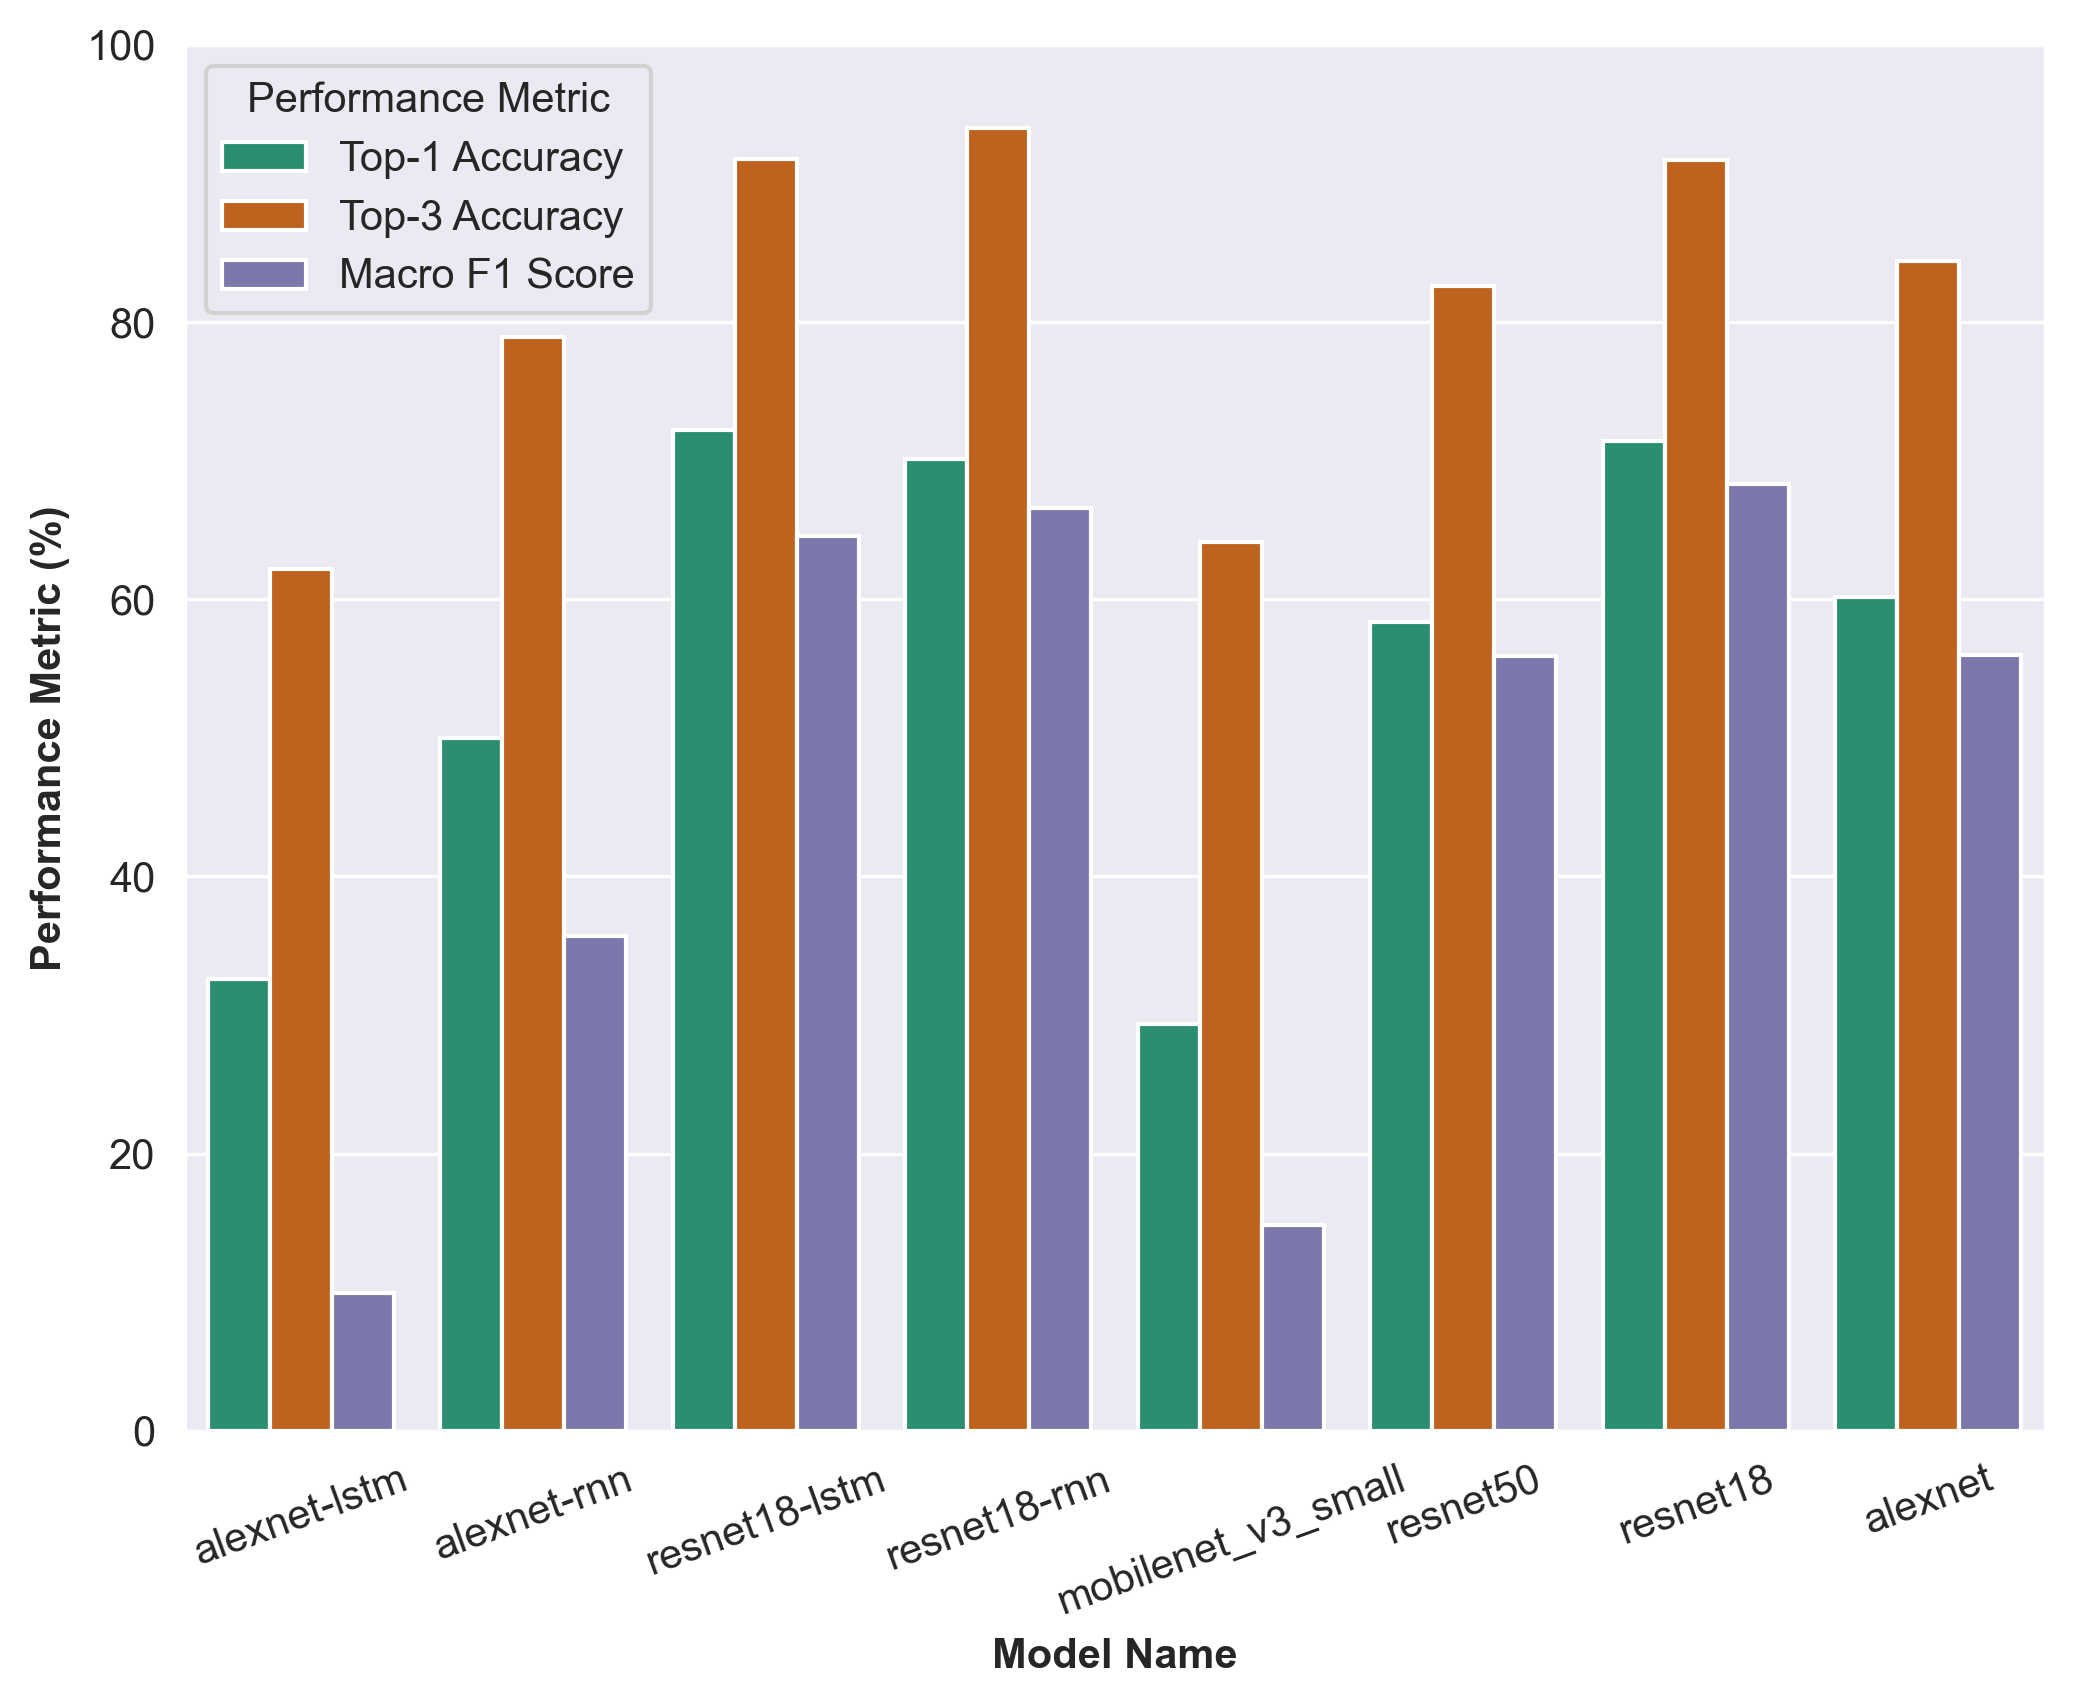
\includegraphics[width=0.65\textwidth]
      {./figures/experiment1-performance-metricz.png}
    \end{center}

    \caption{
    \textbf{Performance Metrics.} The three classification performance metrics
    are shown for all models in a grouped bar chart.
    }

    \label{fig:performance-metrics}
  \end{figure}

  \subsection{Performance Efficiency Trade-Off} % (fold)
  \label{sub:Performance Efficiency Trade-Off}

  The general trend in deep learning is that increasing the number of
  parameters, and thereby the complexity of the model, generally leads to better 
  performance. In this experiment, higher model complexity was reached in two
  ways: Firstly, by increasing the number of parameters in the CNN module, and,
  secondly, by stacking a RNN or LSTM layer on top of the CNN module.
  In order to investigate the performance-efficiency trade-off, the number of
  parameters, the number of floating point operations and the throughput of all
  models were measured and plotted against the Top-1 Test Accuracy. The results
  are shown in Figure~\ref{fig:performance-efficiency-trade-off}.

  Figure~\ref{fig:performance-efficiency-trade-off} shows the Top-1 Test
  Accuracy of all models against the number of parameters.
  
  \begin{figure}[ht]
    \centering
    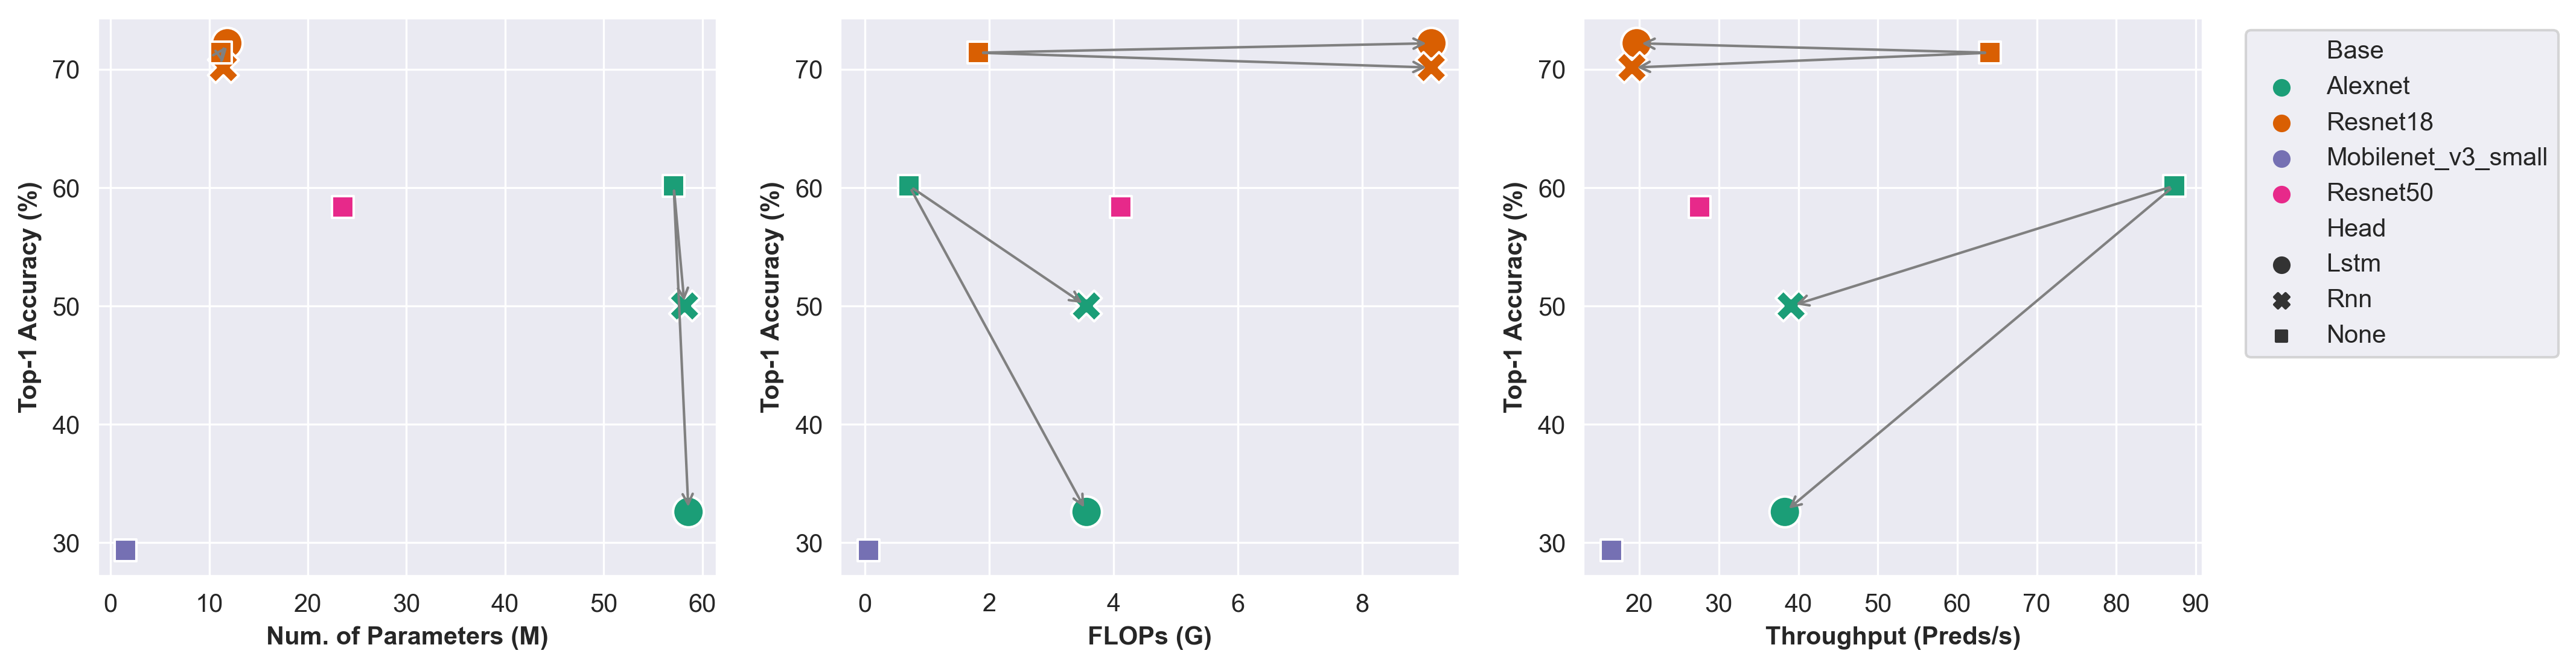
\includegraphics[width=\textwidth]{./figures/experiment1-scatter-plots.png}

    \caption{
      \textbf{Performance-Efficiency Trade-Off.} The three Figures show the
      Top-1 Accuracy (\%) against (a) the number of parameters, (b) the number
      of floating point operations and (c) the throughput (predictions per
      second) for all models. The models are coloured according to their
      CNN base module and the marker style indicates the type of RNN head.
      The grey lines aid the visualisation of the development of
      performance-efficiency trade-off with different recurrent modules.
    }

    \label{fig:performance-efficiency-trade-off}
  \end{figure}

  It can be seen that higher model complexity generally does not lead to higher
  performance. Both ResNet50 and AlexNet have significantly more parameters than
  ResNet18, but perform worse. The picture is slightly different for the number
  of floating points operations and throughput. As expected, ResNet50, due to
  its higher number of parameters, requires more floating point operations
  during inference, which leads to a lower throughput. However, AlexNet, despite
  being almost 6x larger than ResNet18 in terms of pure parameter count, has a
  lower number of floating point operations and a higher throughput. However,
  since the base ResNet18 model already has a throughput of ~65 frames per
  second, which is more frames per second than most modern cameras capture, the
  throughput does not seem to be a limiting factor.

  % subsection subsection name (end)
  
  % subsection subsection name (end)

  \subsection{Temporal Dimension} % (fold)
  \label{sub:Temporal Dimension}

  One of the main difference in the trained models is whether or not they are
  capable of processing the temporal nature of the video frames. It was
  hypothesised that the CNN-RNN video classification models would perform better
  due to an increased number of features and the ability to learn temporal
  information from the video frames. The results show that this is not the case.

  Figure~\ref{fig:performance-efficiency-trade-off} not only shows the
  performance-efficiency trade-off, but also the difference in performance and
  efficiency between the base CNN modules and the CNN-RNN models. The grey lines
  connect the base CNN module with the CNN-RNN model. It can be seen that adding
  the RNN head leads to unchanged (ResNet18) or decreased (AlexNet) performance,
  and significantly higher number of floating point operations and therefore
  lower throughput. The analysis clearly shows that adding a RNN head does not
  yield the desired effect of modelling the temporal dimension of the video
  frames to increase the robustness of continuous predictions. Instead, it
  merely increases the model complexity and inference time, which make it
  overall inferior to their pure CNN counterparts.

  \subsection{Data Efficiency} % (fold)
  \label{sub:Data Efficiency}

  Approaching indoor localisation as a classification task, means to frame it as
  a supervised learning problem. Supervised learning requires human-annotated
  training data, which can be prohibitive to obtain in large quantities. For the
  proposed approach to be valid, minimal effort in the initial data collection
  and annotation should be required. For this reason, the second experiment
  tries to find an answer for the research question: \textit{ ``How much data
  is necessary to achieve good performance''}. To answer this question, a single
  image and video classifier are chosen and trained on different subsets of the 
  training data. The subsets include $10\%$, $20\%$, $30\%$, $40\%$, $50\%$,
  $60\%$, $70\%$, $80\%$, $90\%$ and $100\%$ of the training data. The models 
  are then evaluated as outlined in Section~\ref{sub:evaluation} to find the
  natural drop-off in performance as the amount of training data decreases.


  % data-efficient learners (figure: ratio-vs-performance)

  \begin{figure}[ht]
    \centering
    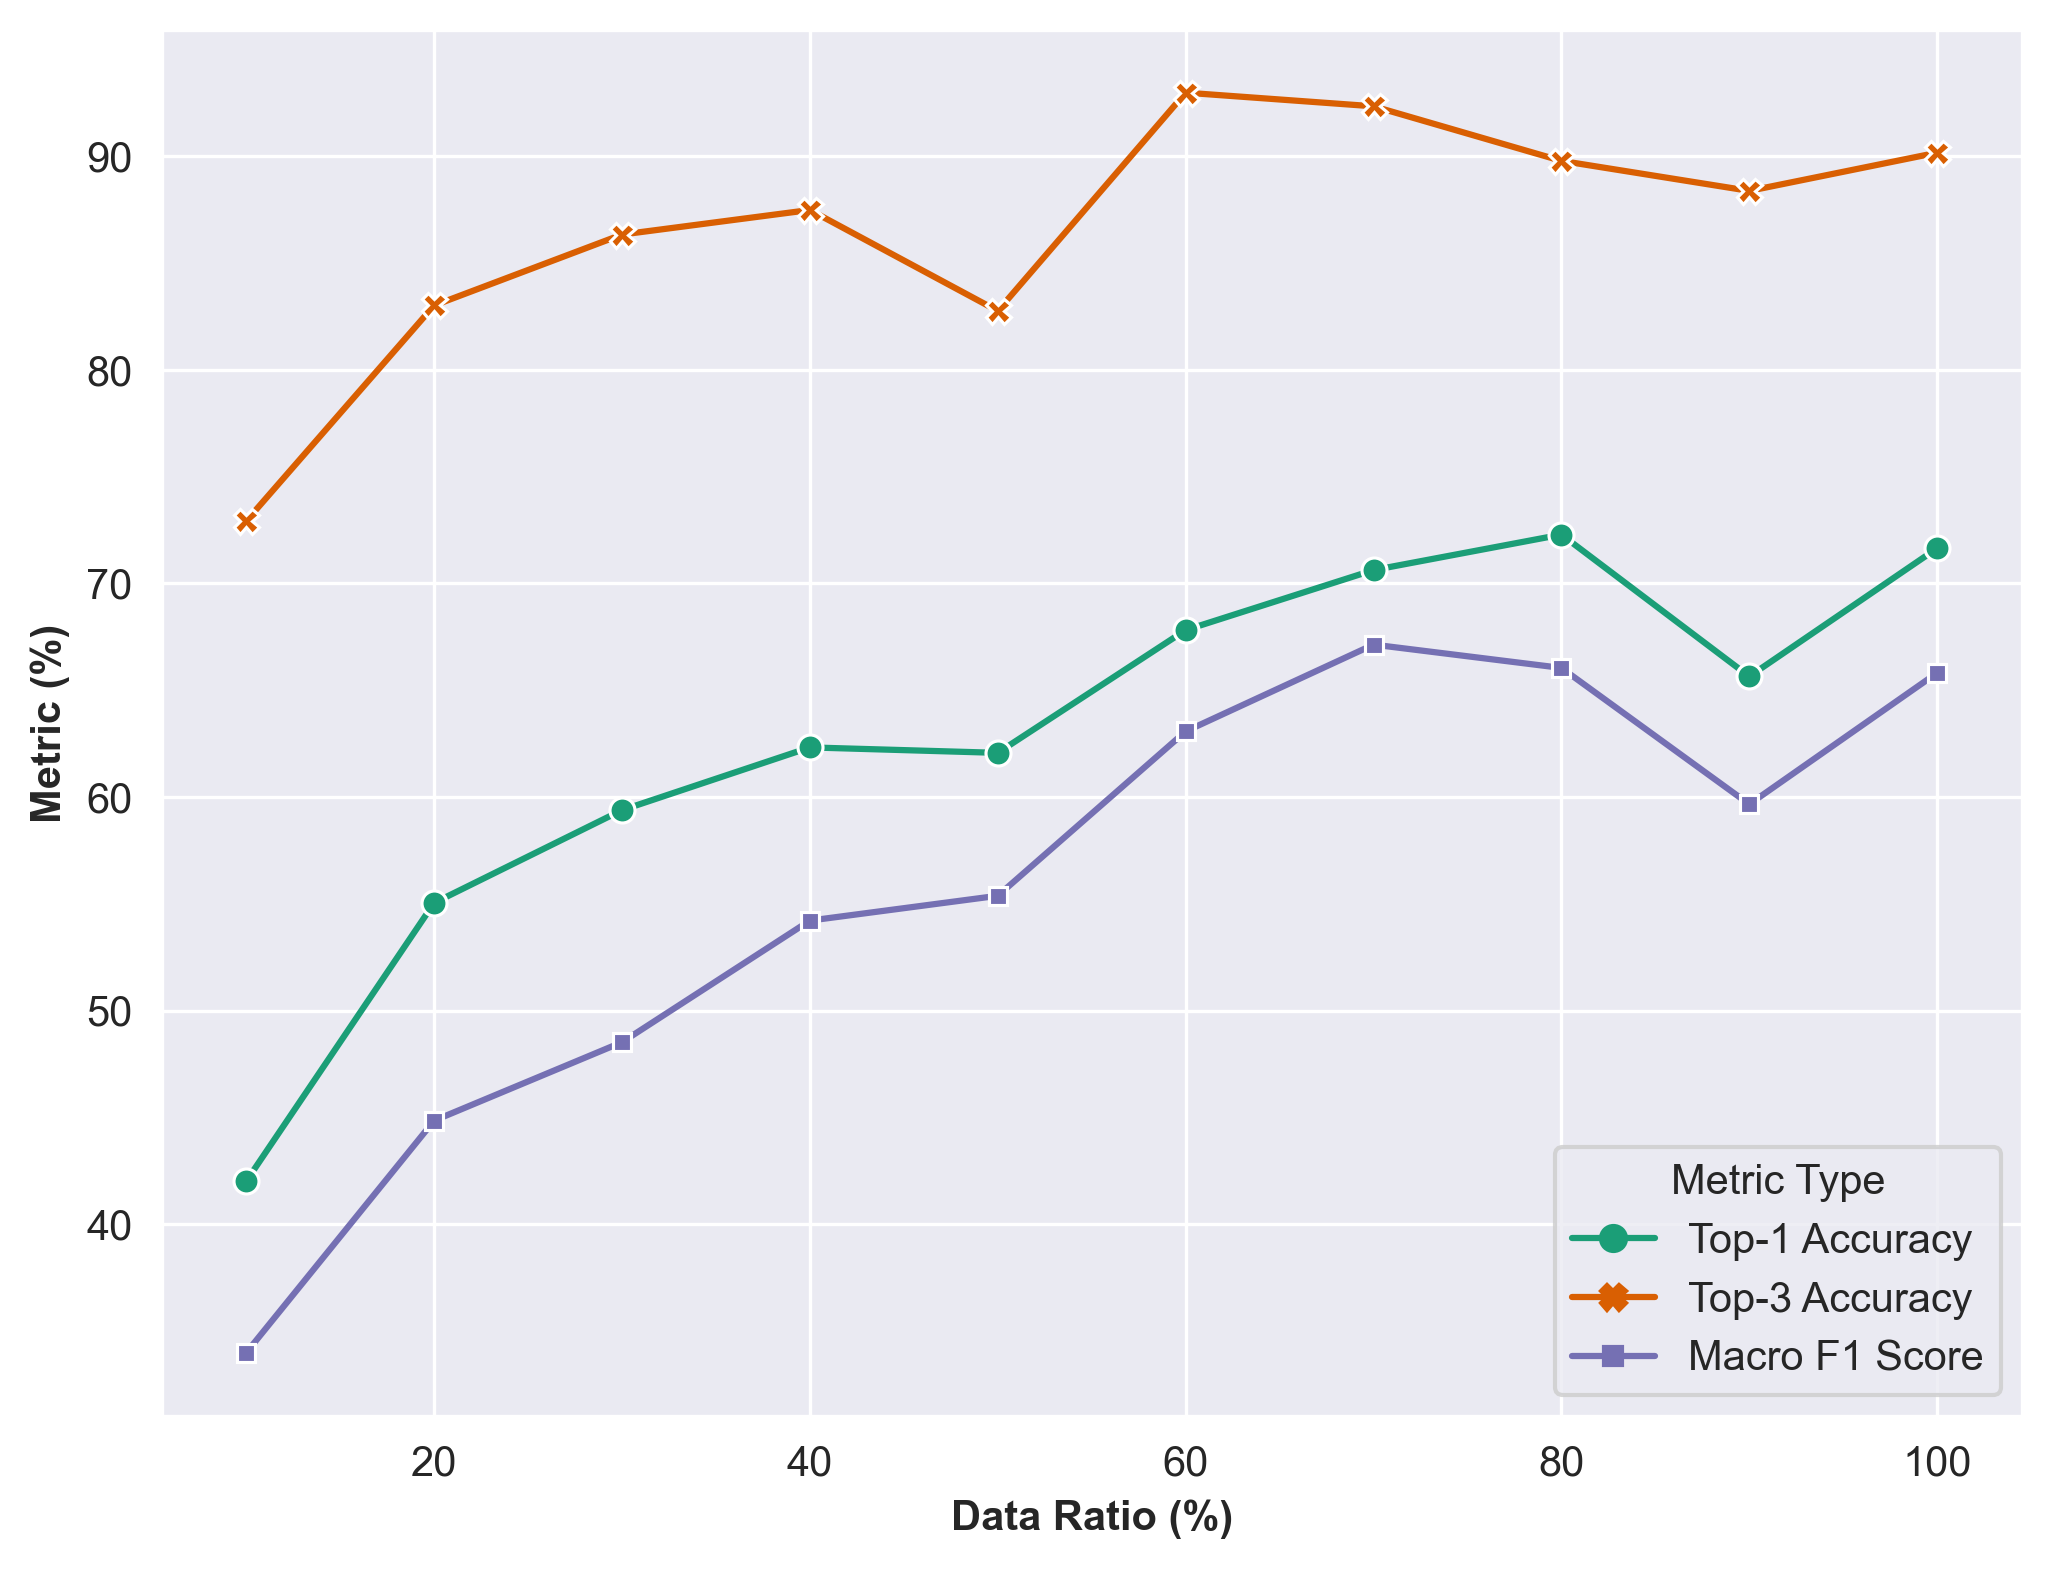
\includegraphics[width=0.8\textwidth]{./figures/experiment2-ratio-vs-performance.png}
    \caption{
      \textbf{Data Efficiency.} The figure shows the performance of the baseline
      model \texttt{resnet18} when trained on different training data metrics.
    }
    \label{fig:data-efficiency}
  \end{figure}
  
  
  % subsection subsection name (end)

  
  
  % subsection subsection name (end)
  
  \subsection{Analysing Failing Scenarios: Mispredicted Samples} % (fold)
  \label{sub:Analysing Failing Scenarios: Mispredicted Samples}

  To better understand the strengths and weaknesses of the best-performing
  model, a pure ResNet18 CNN module, the confusion matrix is analysed.
  Figure~\ref{fig:resnet18-confusion-matrix} shows the confusion matrix of the
  ResNet18 model.

  \begin{figure}[ht]
    \centering
    \begin{subfigure}[b]{0.49\textwidth}
      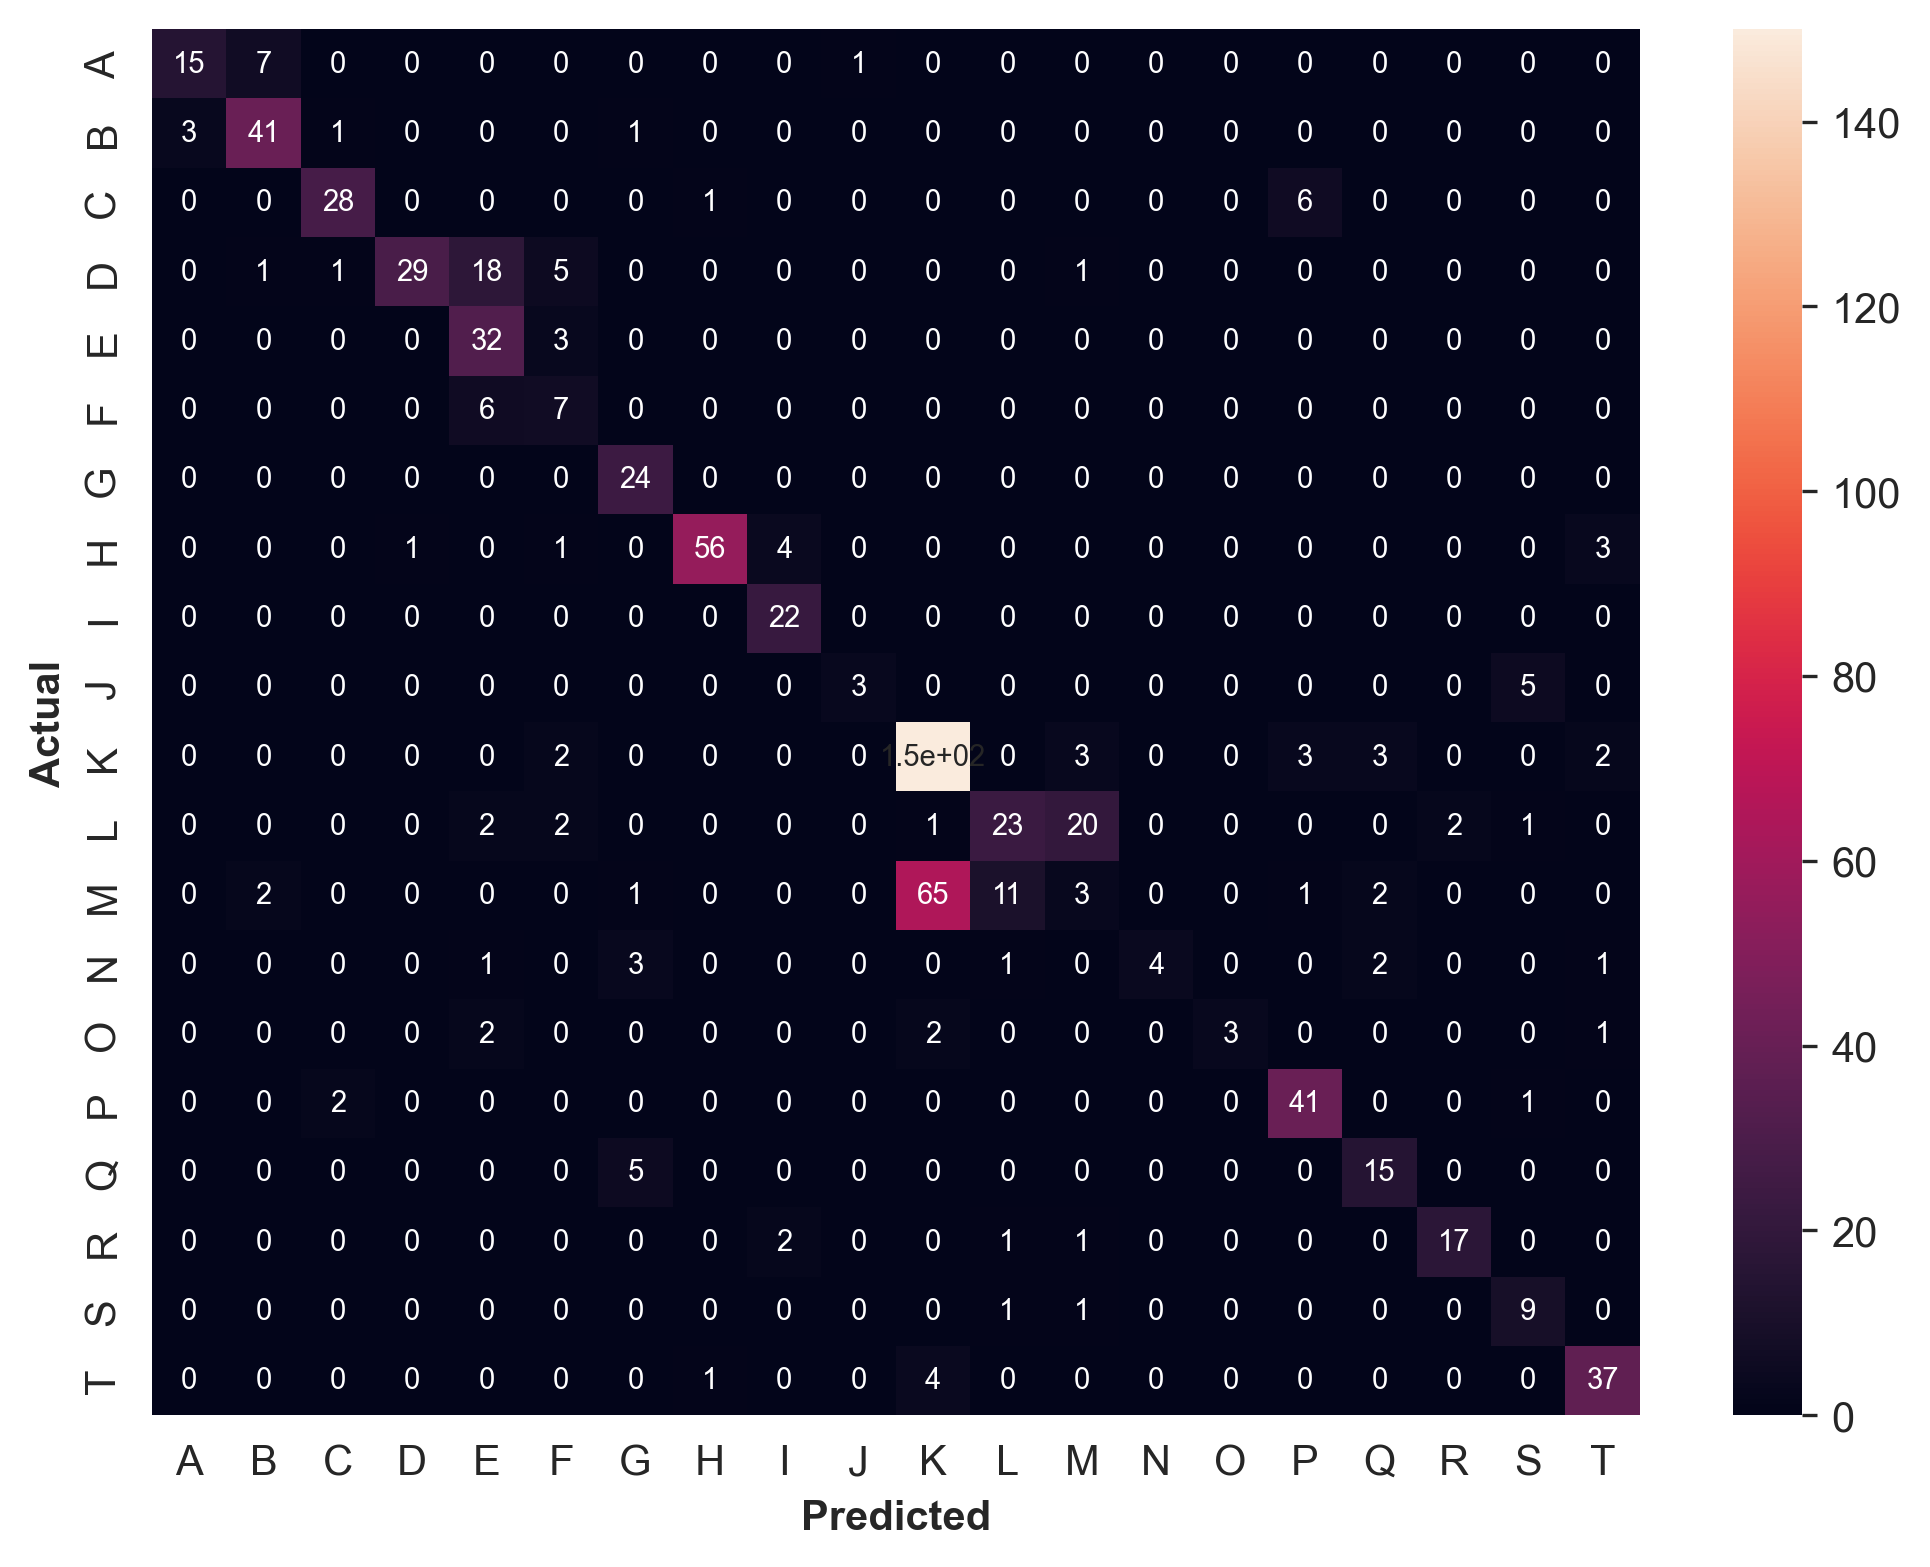
\includegraphics[width=\textwidth]{figures/experiment1-conf-matrix-resnet18.png}
      \caption{Unnormalised Confusion Matrix}
    \end{subfigure}
    \begin{subfigure}[b]{0.49\textwidth}
      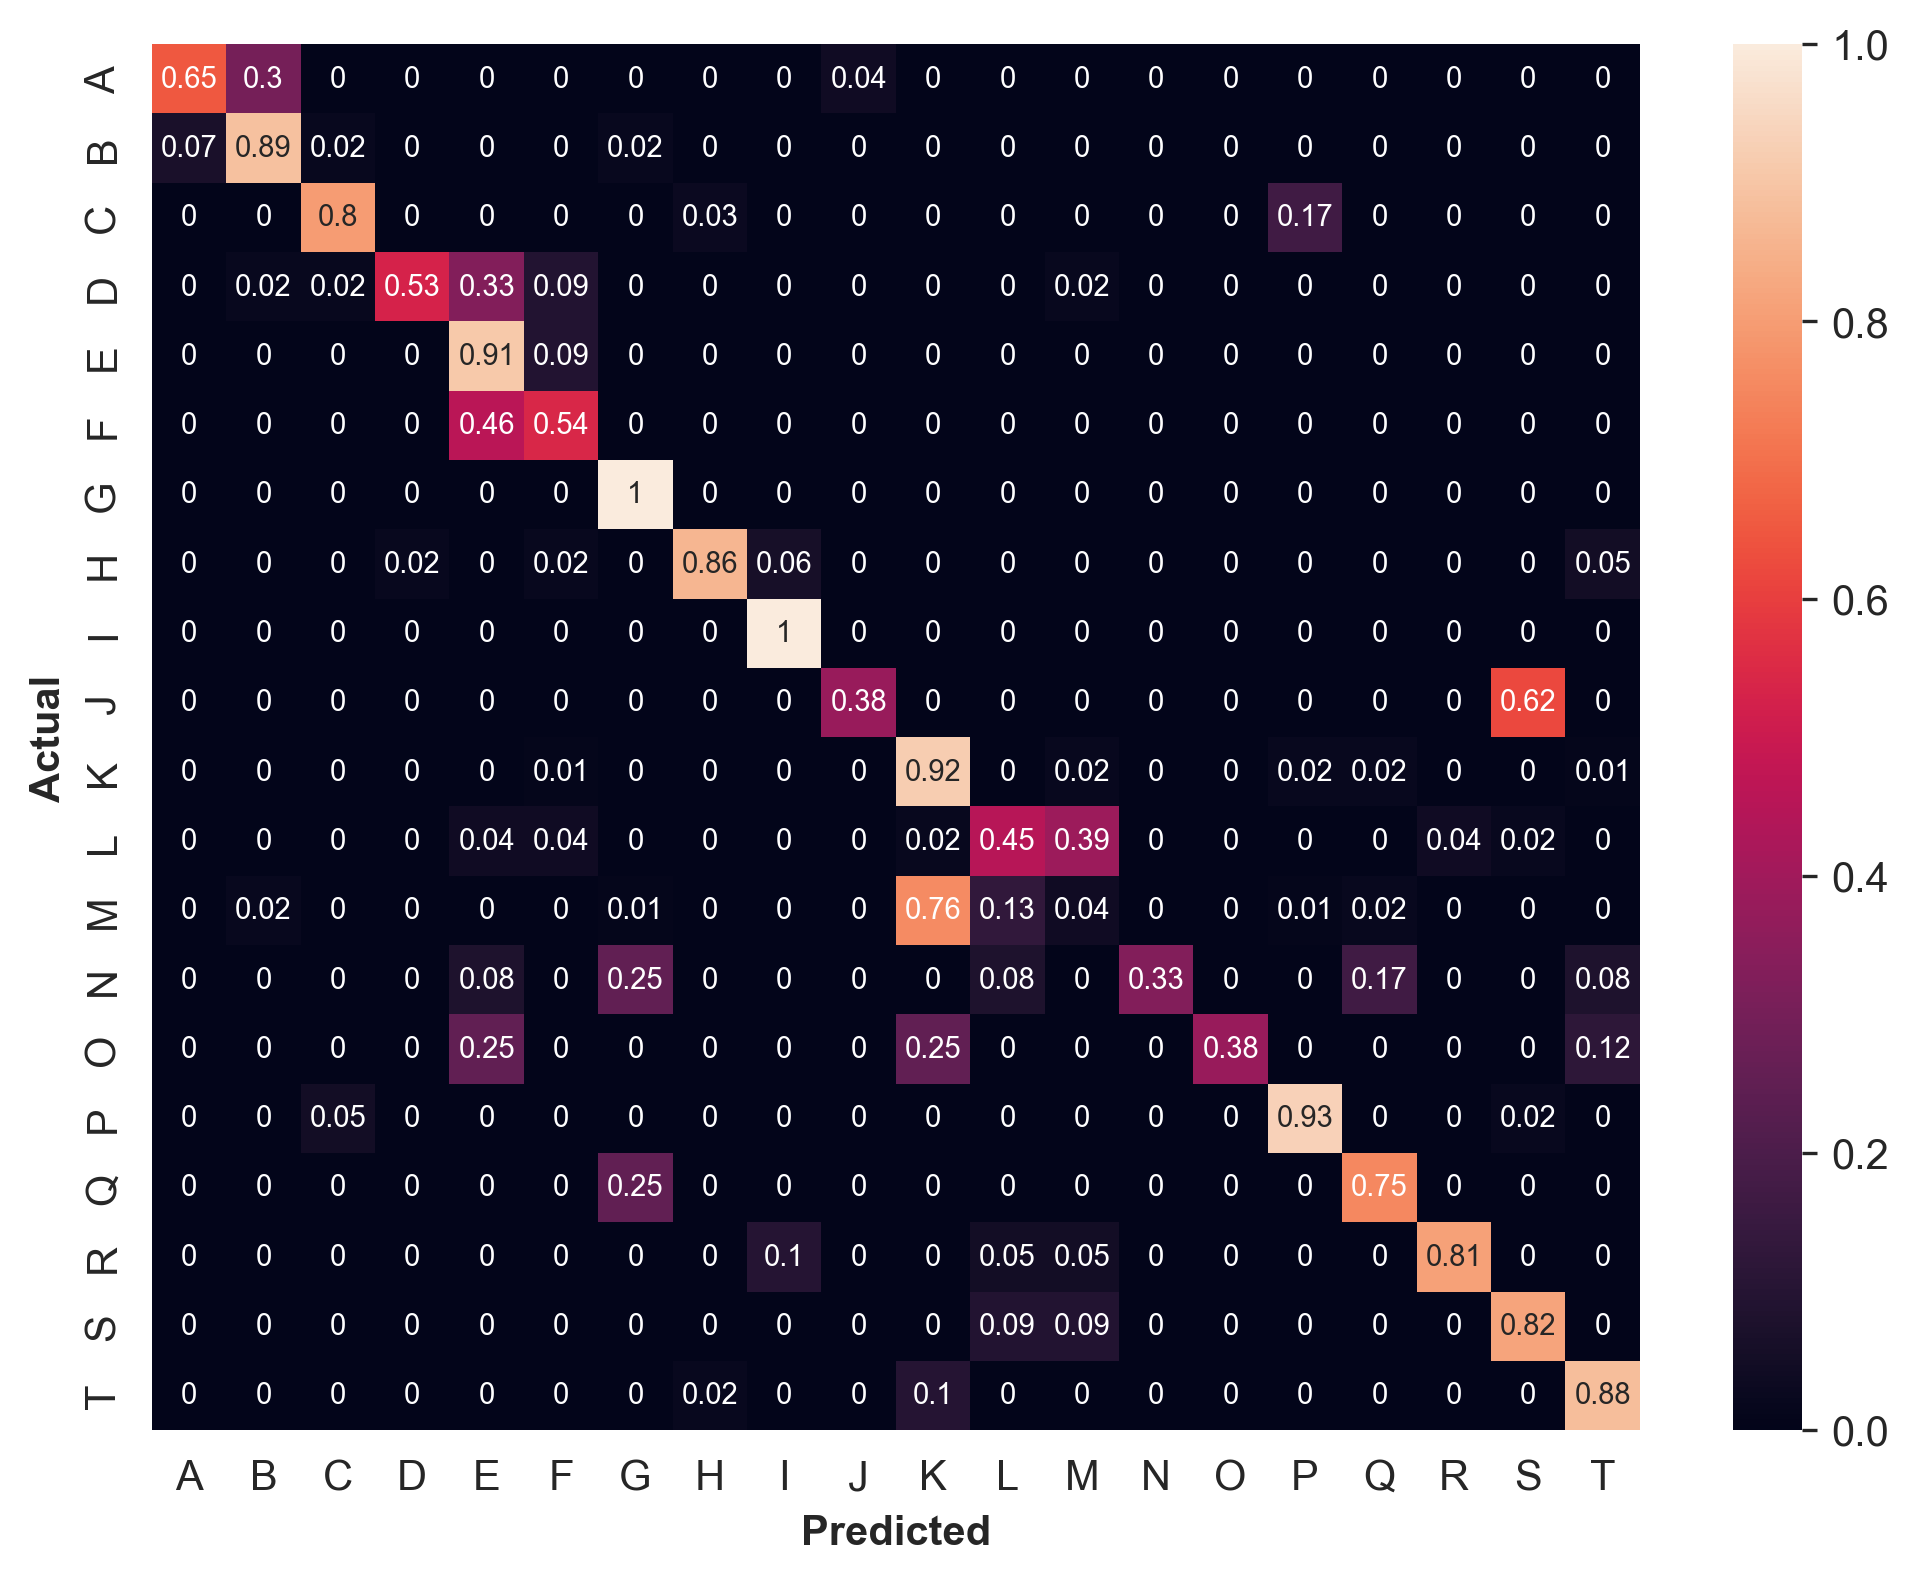
\includegraphics[width=\textwidth]{figures/experiment1-recall-matrix-resnet18.png}
      \caption{Row-Normalised Confusion Matrix}
    \end{subfigure}
    \caption{
      \textbf{ResNet18 Confusion Matrix.} The figure shows the (a) unnormalised
      and (b) row-normalised confusion matrix. For (a), the entry at row $i$ and
      column $j$ shows the number of samples that belong to class $i$ but were
      predicted to be class $j$. For (b), the entry at row $i$ and column $j$
      shows}
    \label{fig:resnet18-confusion-matrix}
  \end{figure}
  
  % subsection Mispredicted Samples (end)

  \subsection{Extracting Characteristics of the Model using GradCam} % (fold)
  \label{sub:Mispredicted Samples}

  % qualitative characteristics of resnet18: gradcam

  % subsection Mispredicted Samples (end)

  \subsection{Deployment on Mobile Devices}
  \label{sub:deploment}

  As a proof of concept, the best-performing model, was deployed on a mobile
  device. The trained model was first quantised to 8-bit float precision and
  then converted to \texttt{TorchScript} format. The \texttt{TorchScript} model
  was then deployed on a mobile device using the \texttt{PlayTorch}
  framework~\textit{[CITE]}. The \texttt{PlayTorch} framework is a port of the
  PyTorch Mobile SDK that is natively compatible with native iOS and Android
  Deployment to Javascript. This allows for rapid prototyping and deployment of
  PyTorch models on mobile device using the popular React Native framework and
  Expo. The model runs locally on the device and therefore does not require any
  internet connection after initially downloading the model upon opening the
  app.

  \begin{figure}[ht]
    \centering
    
\includegraphics[width=0.5\textwidth]{./figures/playtorch-qr.png}
    \caption{
      \textbf{PlayTorch App.} Download the PlayTorch iOS or Android app and scan
    the QR code to try out the model on your mobile device.}
    \label{fig:playtorch-qr}
  \end{figure}

  % subsection deployment (end)

  % section Results (end)

  \section{Limitations \& Future Work} % (fold)
  \label{sec:discussion}

  This study has shown the potential of using a pure deep learning pipeline for
  tackling the problem of indoor localisation. However, there are still many
  open questions that need to be addressed in future work for systems similar to
  the approach suggested here to be widely useful in real-world applications.

  % coarse location labels
  The main drawback of the proposed approach is the coarse location labels.
  State-of-the-art indoor localisation systems are able to localise users to
  centimetre accuracy. Therefore, future work should focus making improvements
  on the entire pipeline that allow for higher precision in the location labels.

  % small data set
  Furthermore, this study assumes a small data set of only 40 minutes of video
  footage for training. While the experiment setup allowed to draw conclusion
  about the data efficiency of the models and the general feasibility of the
  data collection and annotation process, it is an open question how similar
  systems scale to even larger indoor spaces with more training data available.

  % representativeness of test split
  Additionally, it has to be noted that the test split was collected over a
  duration of four different days in close succession. Therefore, the test split
  might not be representative of the true variation of visual inputs from a
  indoor location over the course of a year. For example, the location might
  change more significantly than represented in the test split over seasons.
  In that case, the reported test metrics are likely to be over-optimistic. To
  gain confidence in favour or against this hypothesis, monitoring the
  performance of the trained models on test data collected over a longer period
  of time would be necessary.

  % edge-cases
  Finally, the detailed analysis of the mispredicted samples has shown that
  most errors, because the models that show a lot of similar features, such as
  different libraries, or rooms that are architecturally similar across floors.
  Future work should specifically improve on finding solutions to these issues.
  Possible starting points might be to use the fact that sudden jumps in the
  building are impossible, so highly confident predictions from the past can be
  used as a strong indicator for the next room if some knowledge about the
  relative position of the rooms is available.

  % section Discussion (end)

  \section{Conclusion} % (fold)
  \label{sec:conclusion}

  We have shown that the problem of indoor localisation can be phrased as a
  classification problem and be solved through the use of deep learning models
  in a data-efficient manner.
  Simple convolutional neural architectures were able to provide accurate and
  robust predictions and showed emerging learning of features mostly invariant
  to natural variations in the environment.
  The use of a recurrent neural network architecture allowed for the
  incorporation of temporal information and improved the accuracy of the
  predictions, though only marginally so.

  % section conclusion (end)

  % bibliography
  \newpage
  \bibliography{references}
  \bibliographystyle{plain}


  \newpage
  \section{Appendix} % (fold)
  \label{sec:appendix}

  \subsection{Reproducibility} % (fold)
  \label{sub:reproducibility}

  All code and data used in this project is available on GitHub at the
  following link: \url{https://github.com/mikasenghaas/bsc}. The project's 
  \texttt{README} file contains detailed instructions on how to reproduce the
  results of this project.

  Further, the precise configuration and results of the experiments that are
  reported here are publicly available on the Weights \& Biases platform at the
  following link: \url{https://wandb.ai/mikasenghaas/bsc}.

  % subsection reproducibility (end)

  \subsection{Machine Specifications} % (fold)
  \label{sub:machine-specs}

  Table~\ref{tab:machine-specs} lists the specifications of the machine that was
  used for training and evaluation of the models. For training the \texttt{MPS}
  backend was used for accelerated training. However, for inference a single CPU
  core was used, to approximate latency and throughput on mobile devices.


  \begin{table}[ht]
    \centering
    \begin{tabular}{cll}
     \toprule
     & Specification & Value \\
     \midrule

     \multirow{2}{*}{System} & Name & Darwin \\
     \vspace{0.1cm}
     & Node & Local MacBook Pro \\

     \multirow{4}{*}{CPU} & Model & Apple M1 \\
     & Architecture & ARM64 \\
     & Physical Cores & 8 \\
     \vspace{0.1cm}
     & Frequency & 2.4 GHz \\

     \multirow{2}{*}{Memory} & Total Capacity & 16 GB \\
     & Avg. Used Capacity & $\sim 7.4$ GB \\

     \bottomrule
    \end{tabular}
    \caption{Machine Specifications}
    \label{tab:machine-specs}
  \end{table}
  
  % subsection subsection name (end)

  % section remarks (end)

  % conf matrices for all models
  \newgeometry{margin=1cm}
  \begin{figure}[b]
    \centering
    \begin{subfigure}{.33\textwidth}
        \centering
        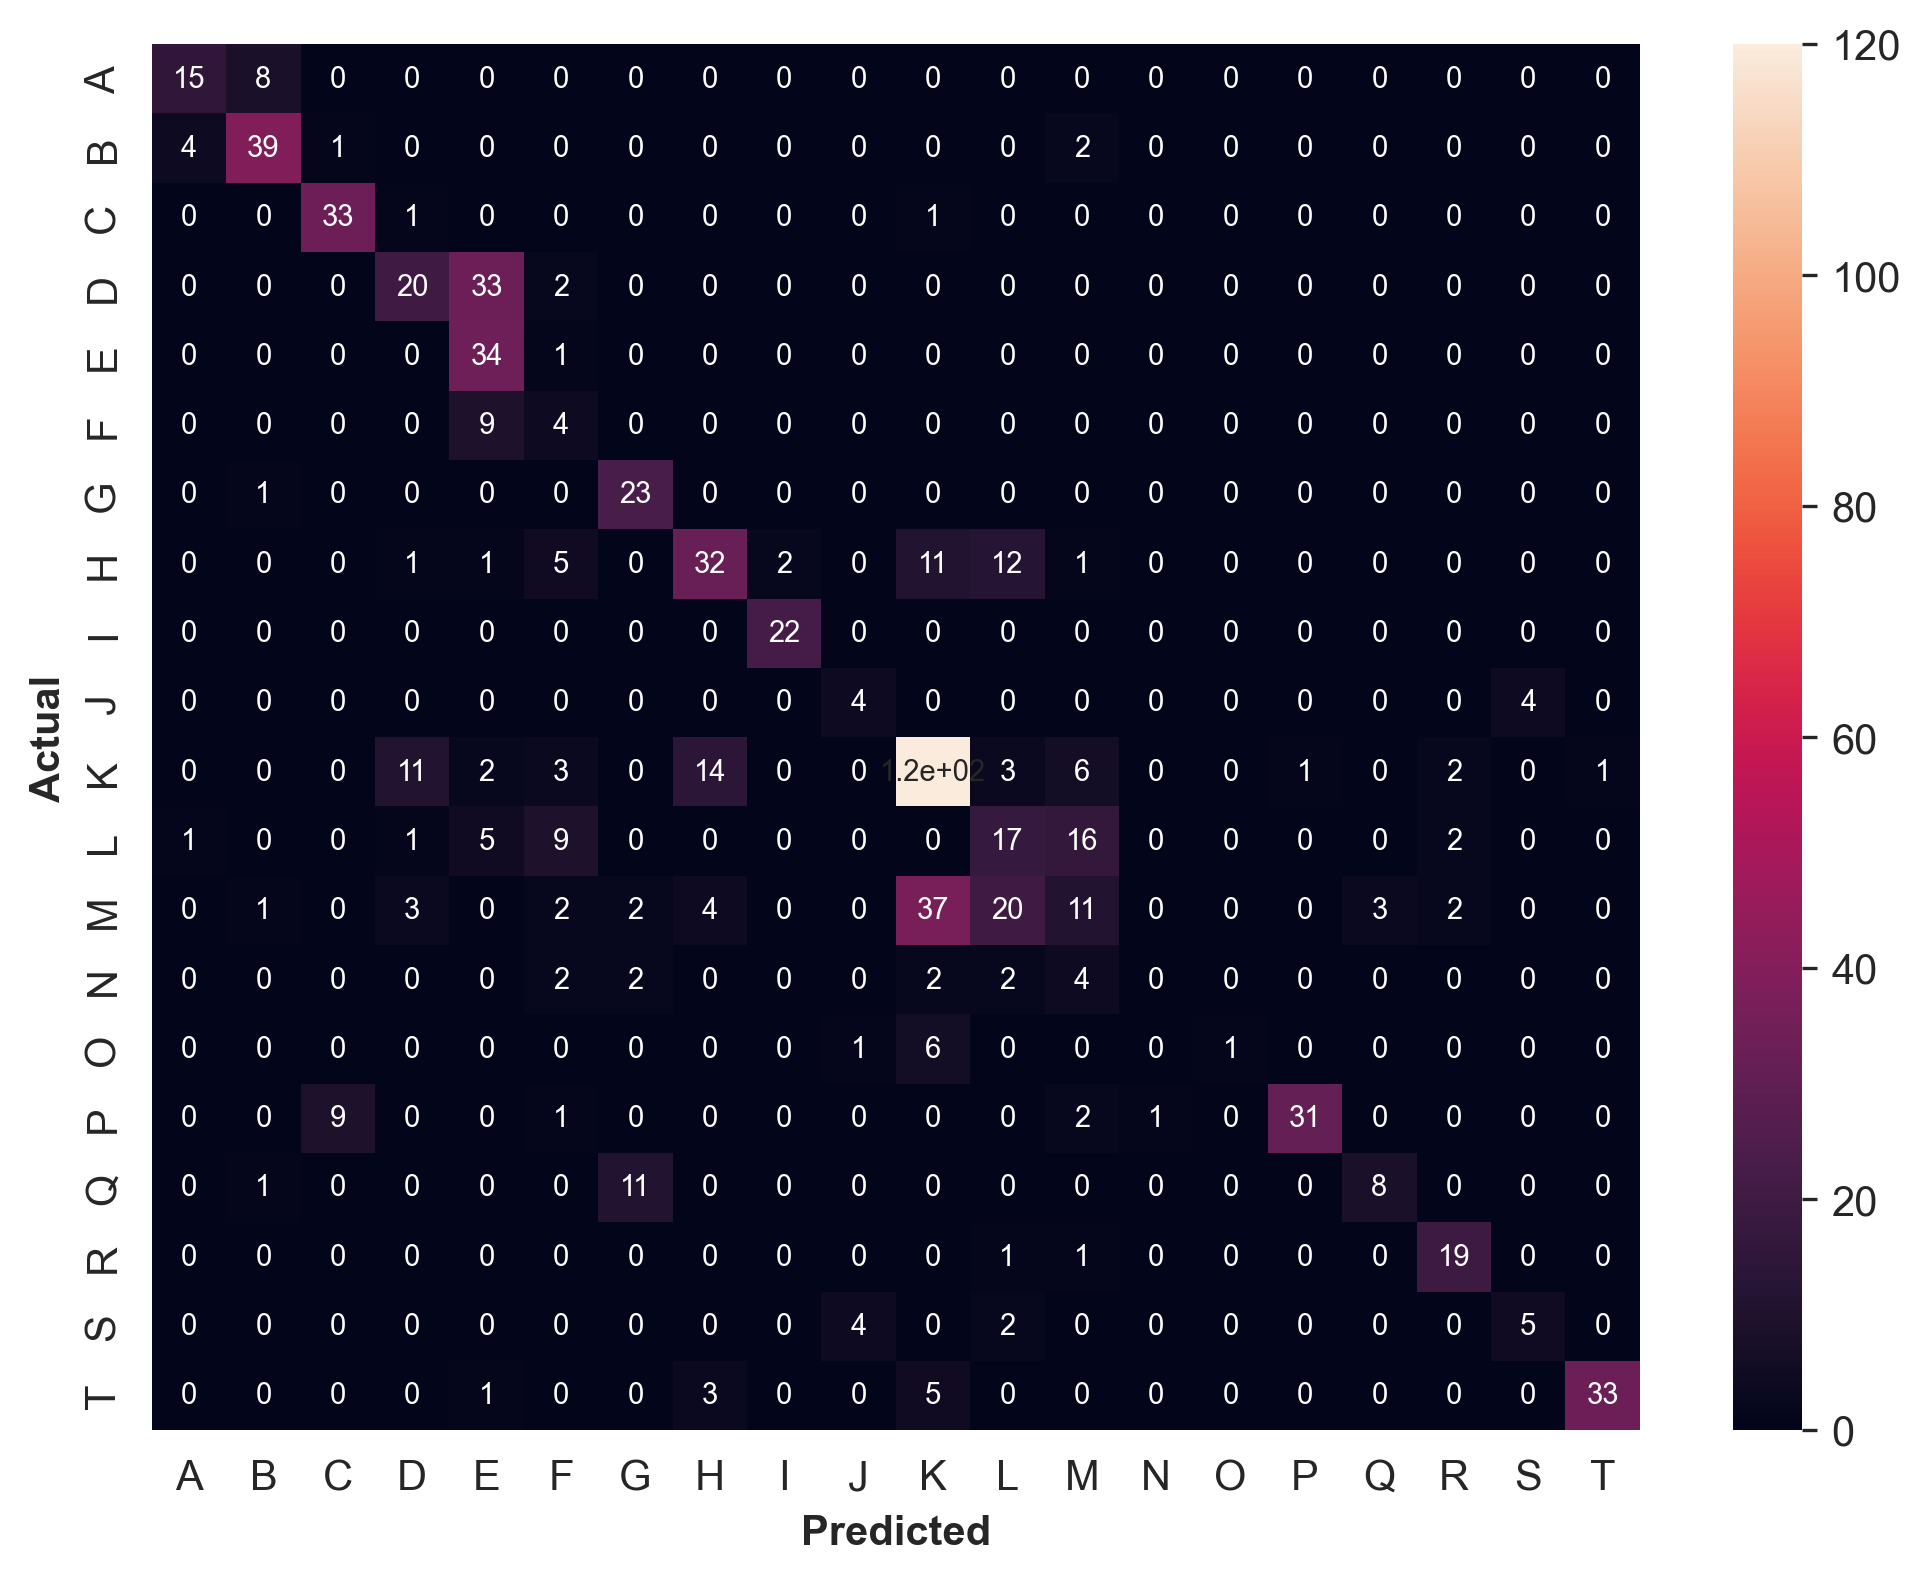
\includegraphics[width=\textwidth]
        {figures/experiment1-conf-matrix-alexnet.png}
        \caption{\texttt{alexnet}}
    \end{subfigure}%
    \begin{subfigure}{.33\textwidth}
        \centering
        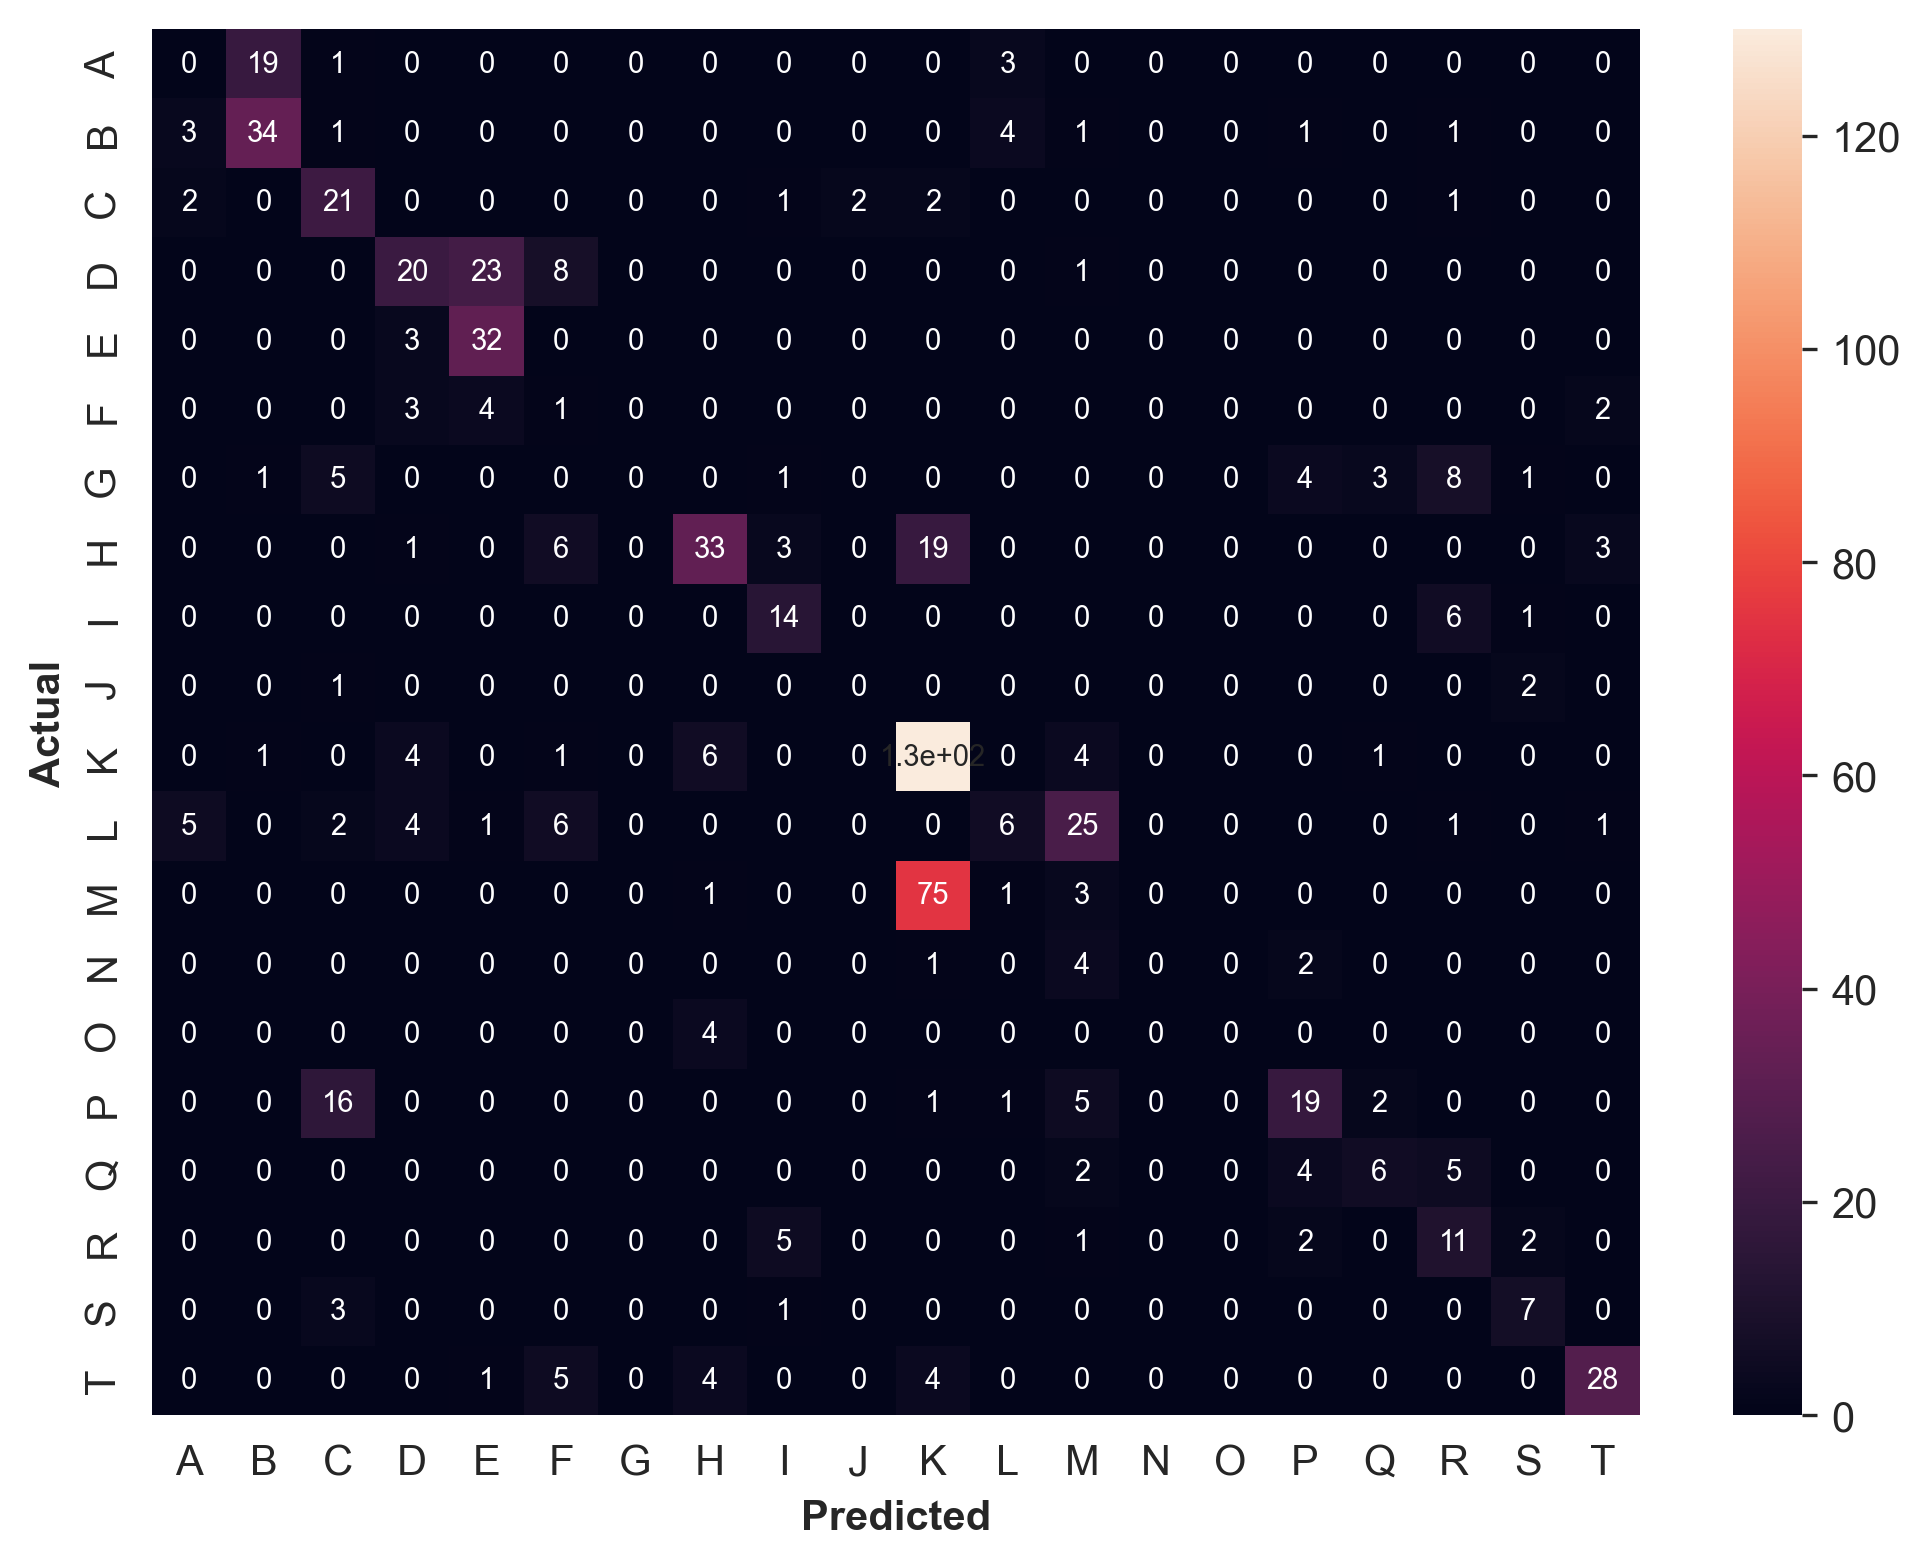
\includegraphics[width=\textwidth]
        {figures/experiment1-conf-matrix-alexnet-rnn.png}
        \caption{\texttt{alexnet-rnn}}
    \end{subfigure}
    \begin{subfigure}{.33\textwidth}
        \centering
        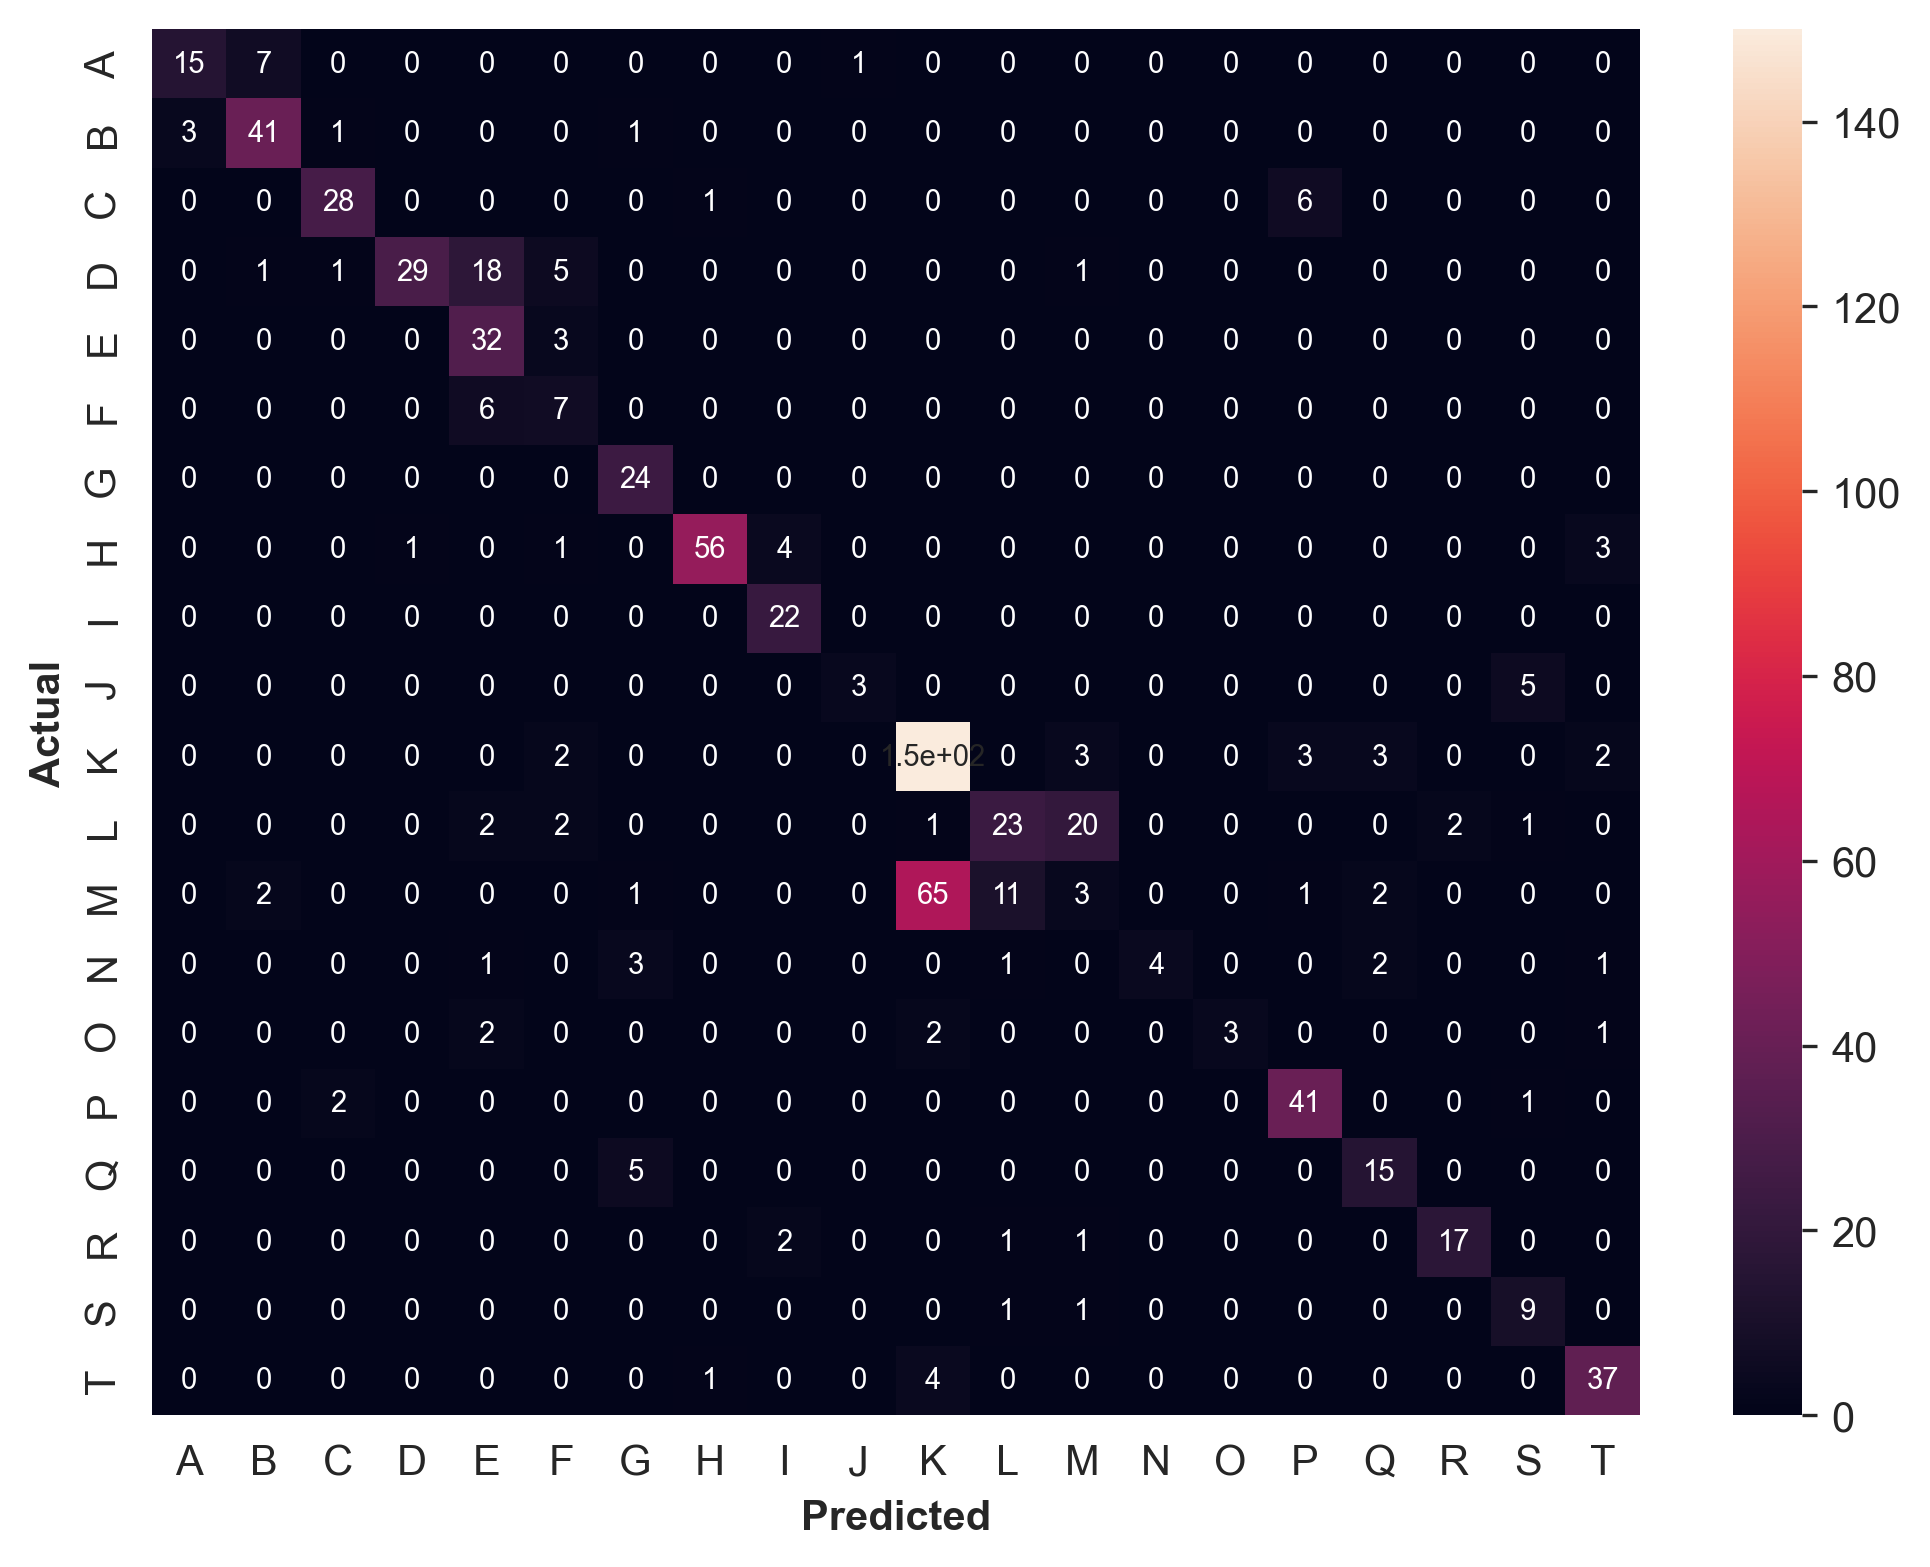
\includegraphics[width=\textwidth]
        {figures/experiment1-conf-matrix-resnet18.png}
        \caption{\texttt{resnet18}}
    \end{subfigure}
    \begin{subfigure}{.33\textwidth}
        \centering
        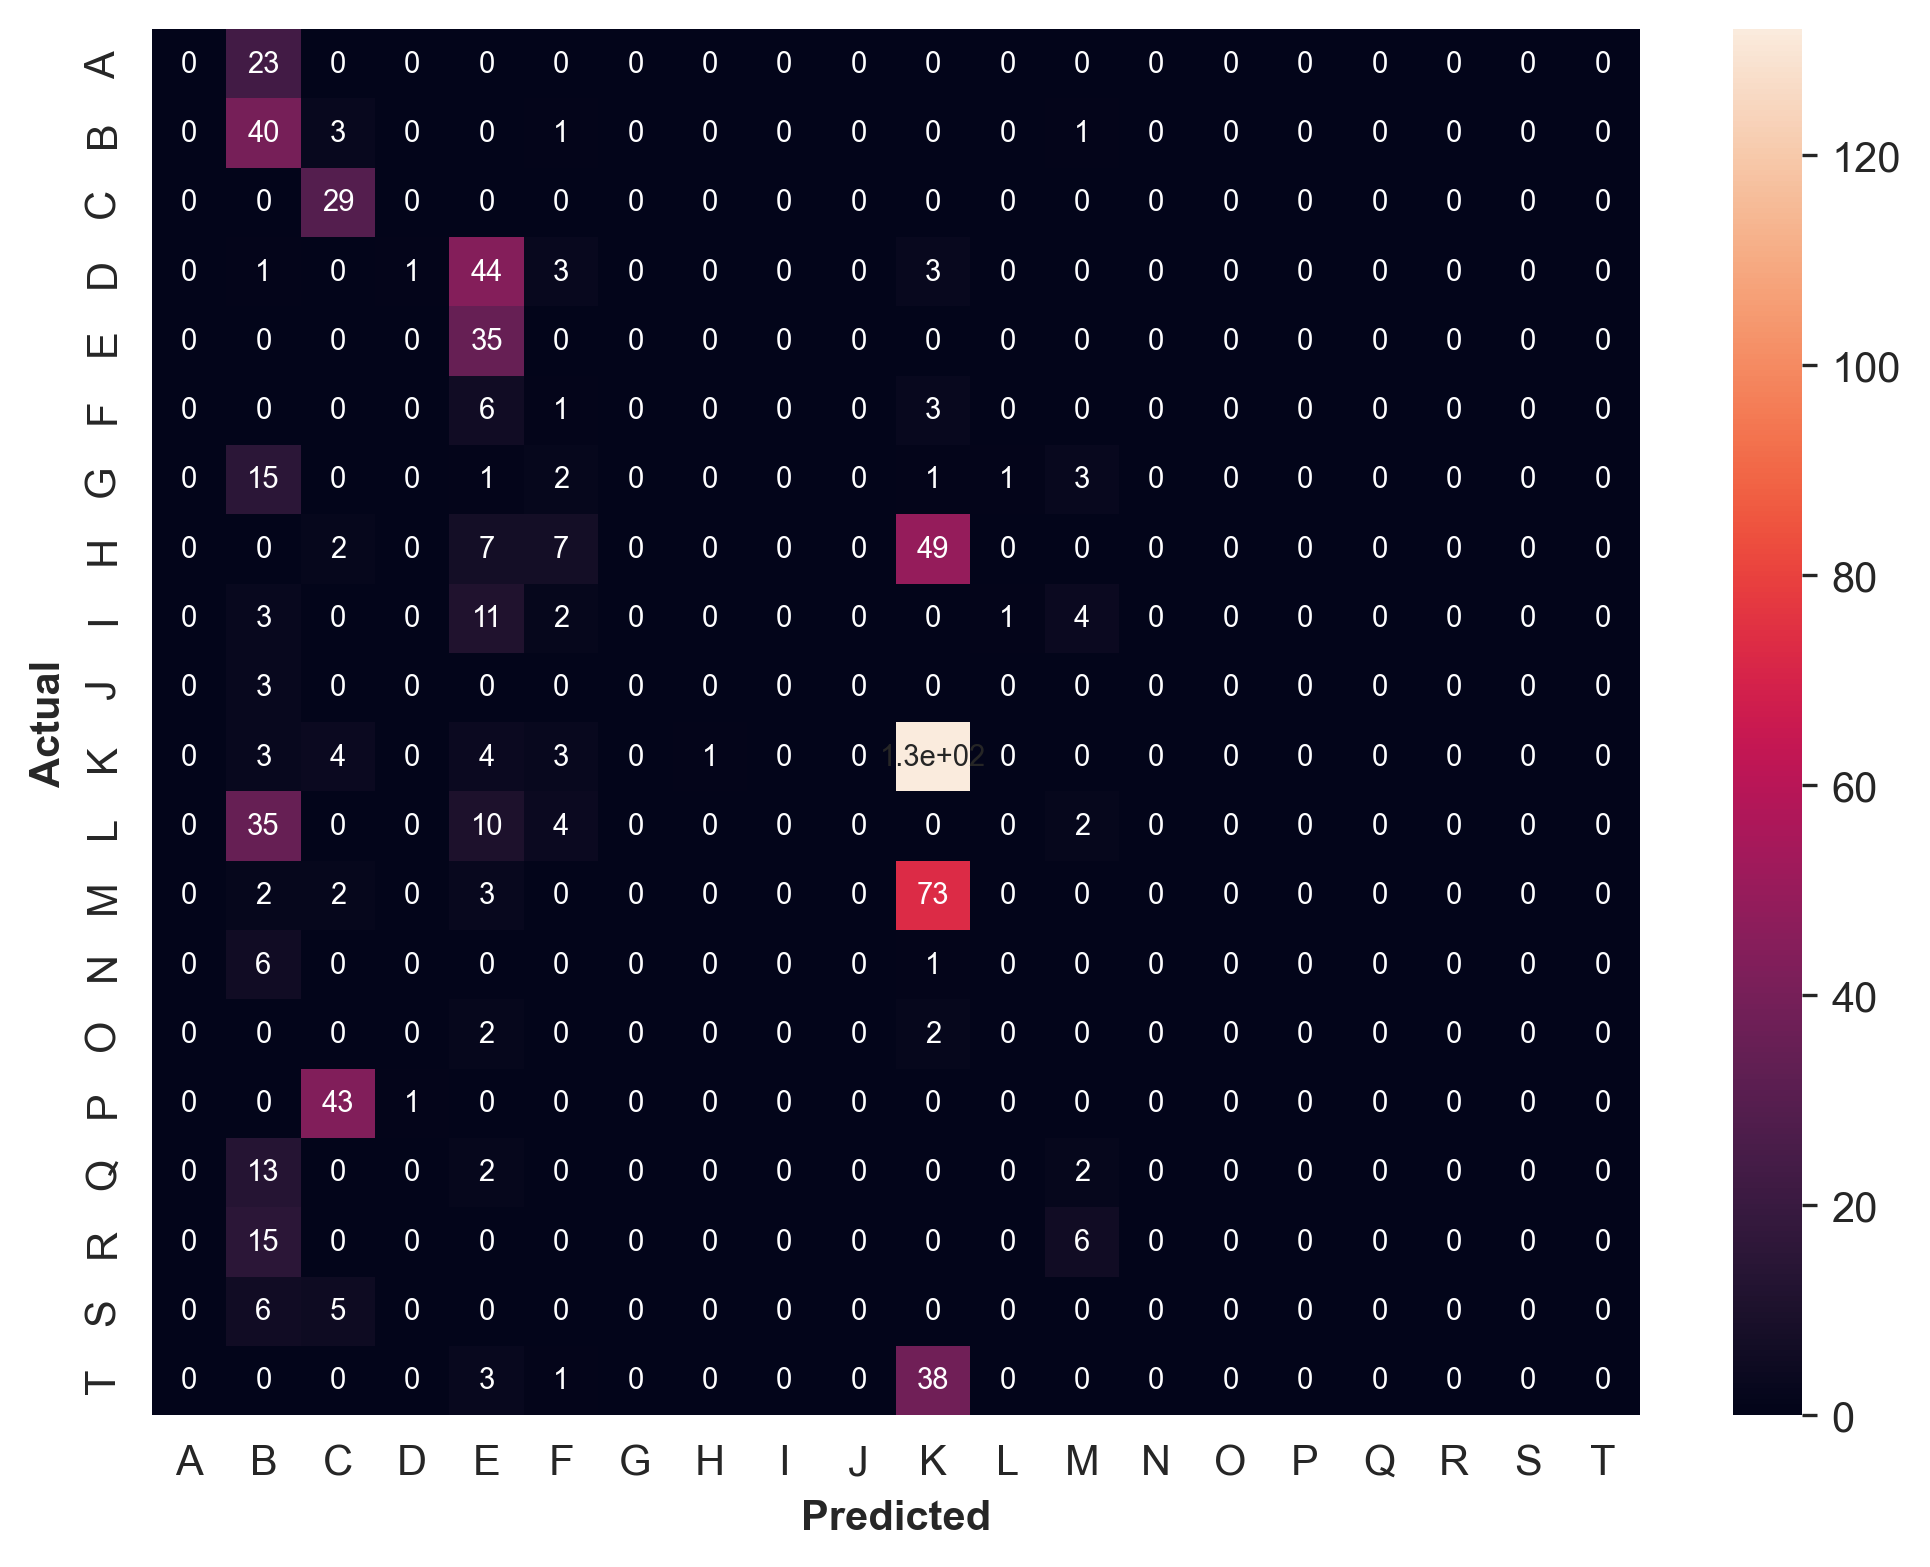
\includegraphics[width=\textwidth]
        {figures/experiment1-conf-matrix-alexnet-lstm.png}
        \caption{\texttt{alexnet-lstm}}
    \end{subfigure}
    \begin{subfigure}{.33\textwidth}
        \centering
        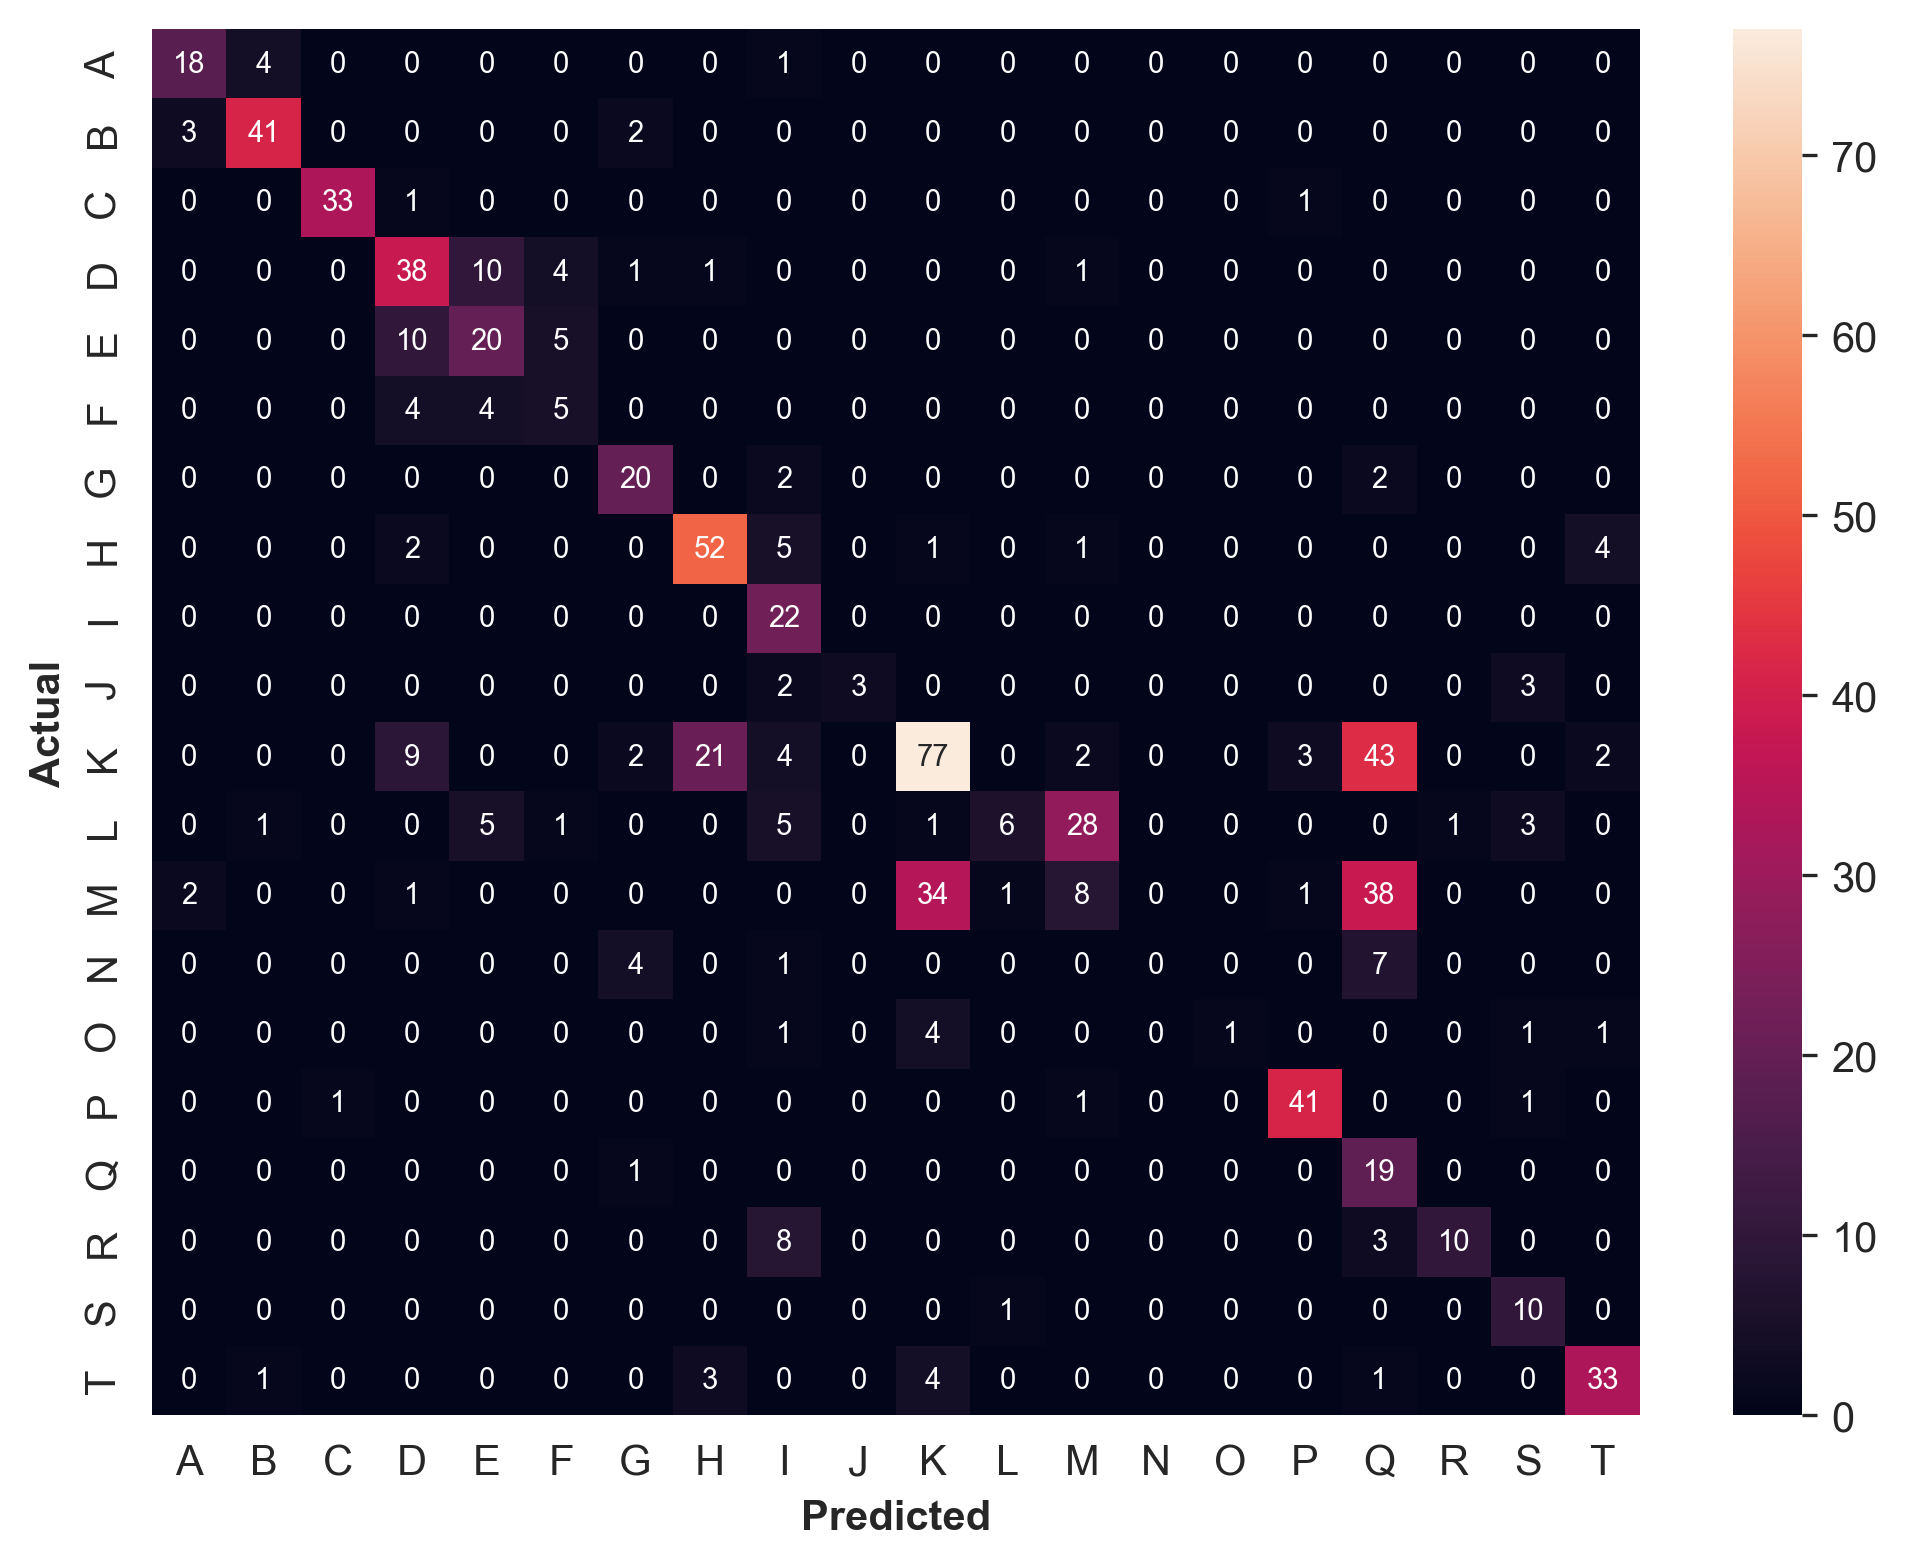
\includegraphics[width=\textwidth]
        {figures/experiment1-conf-matrix-resnet50.png}
        \caption{\texttt{resnet50}}
    \end{subfigure}%
    \begin{subfigure}{.33\textwidth}
        \centering
        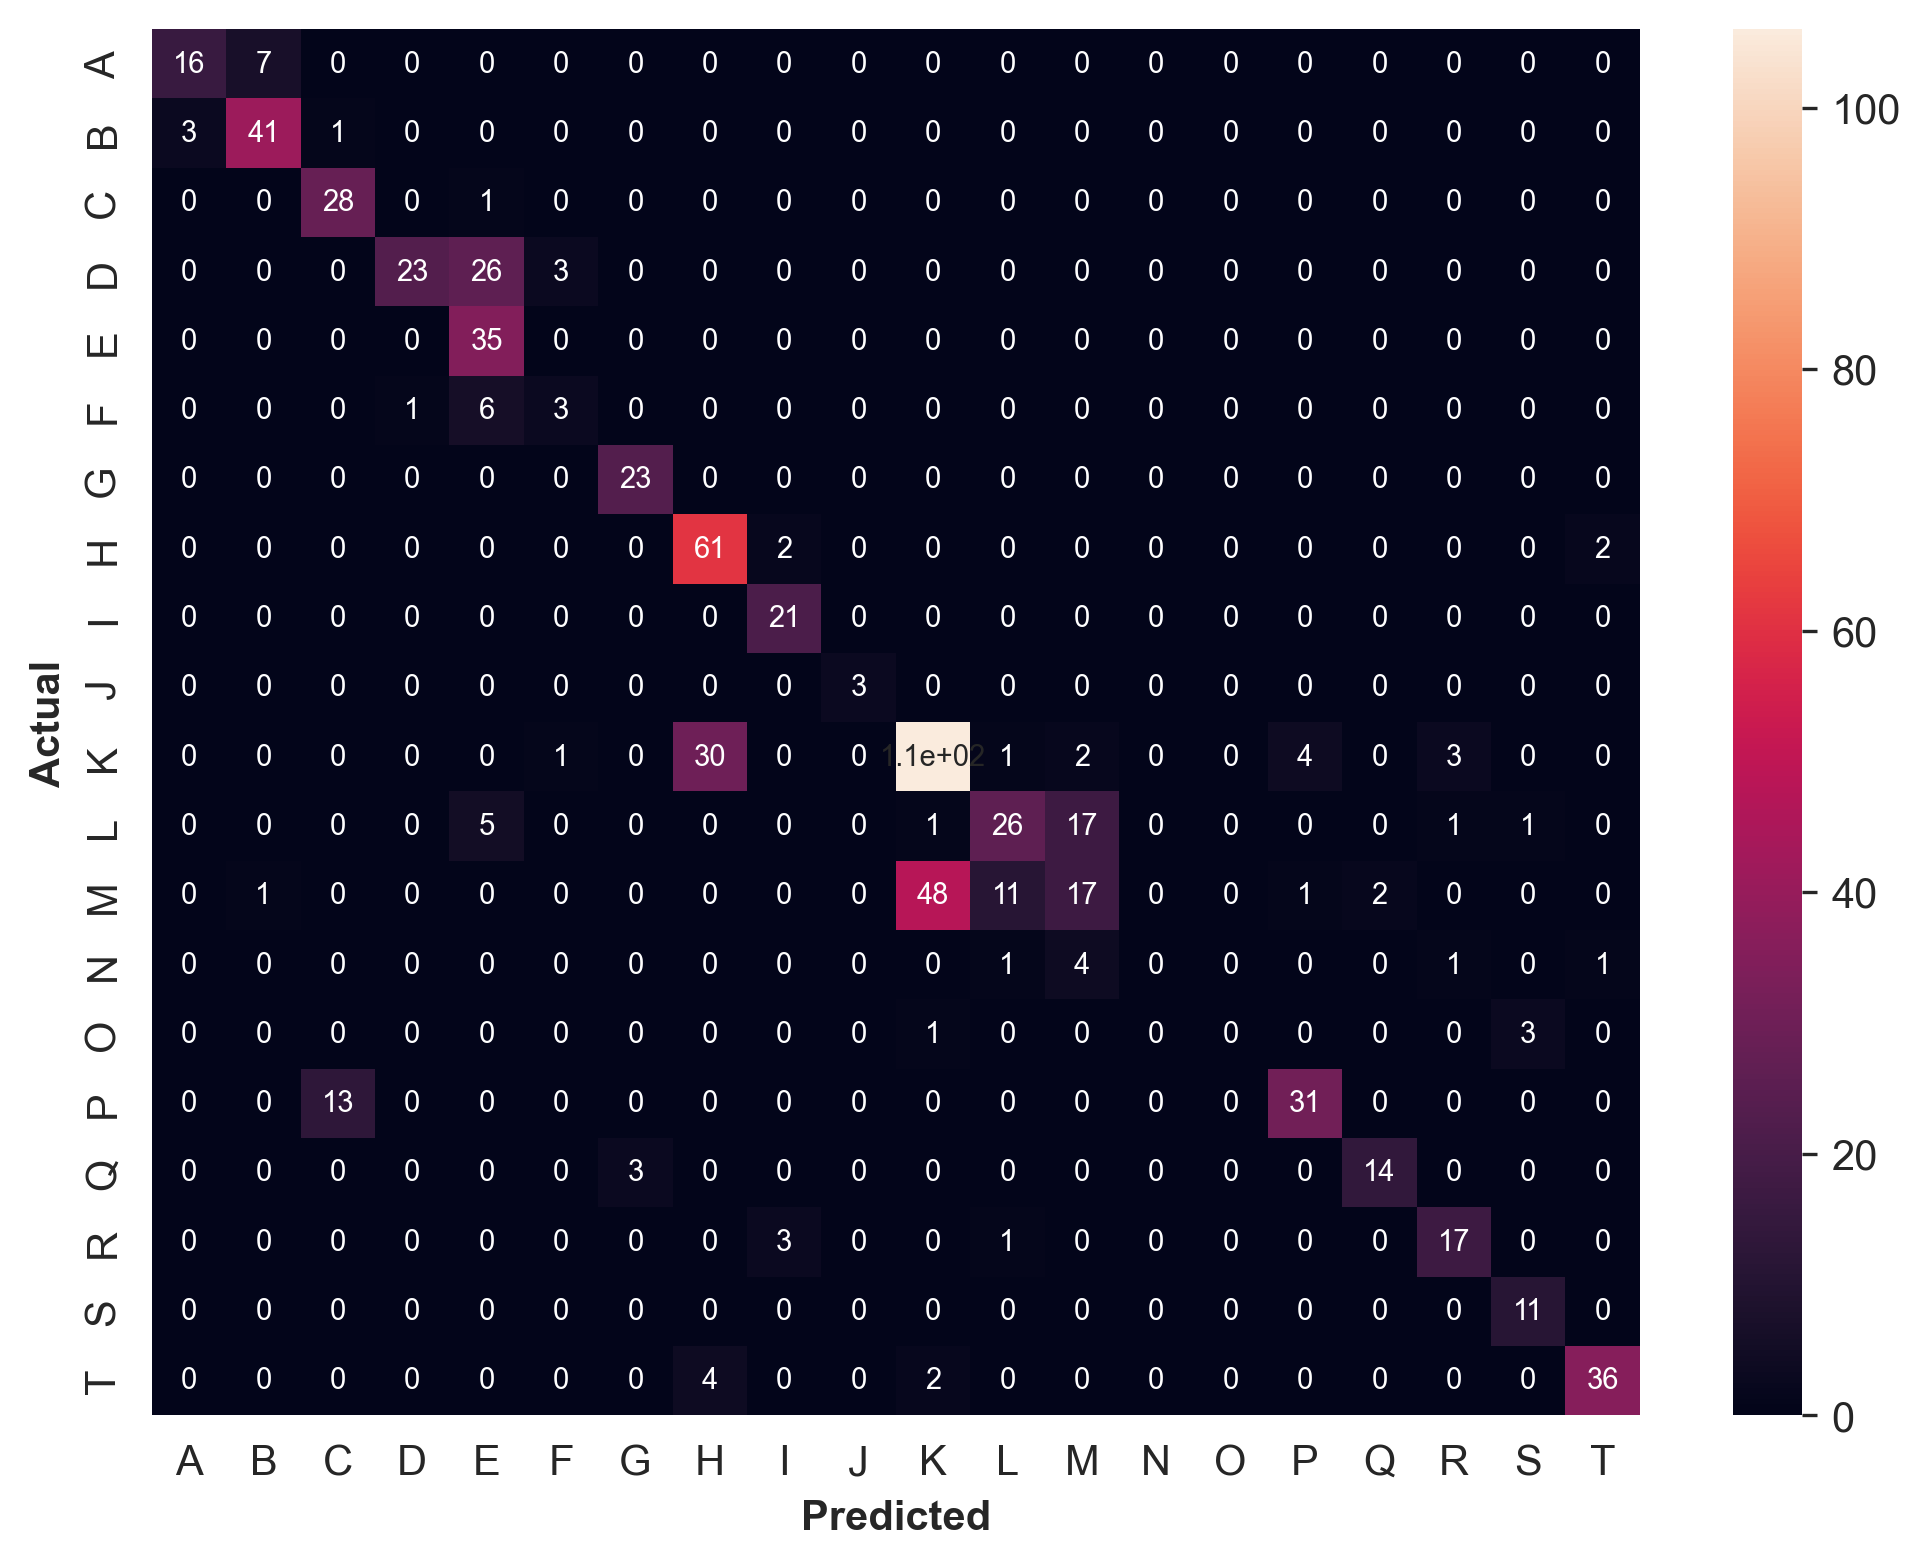
\includegraphics[width=\textwidth]
        {figures/experiment1-conf-matrix-resnet18-rnn.png}
        \caption{\texttt{resnet18-rnn}}
    \end{subfigure}
    \begin{subfigure}{.33\textwidth}
        \centering
        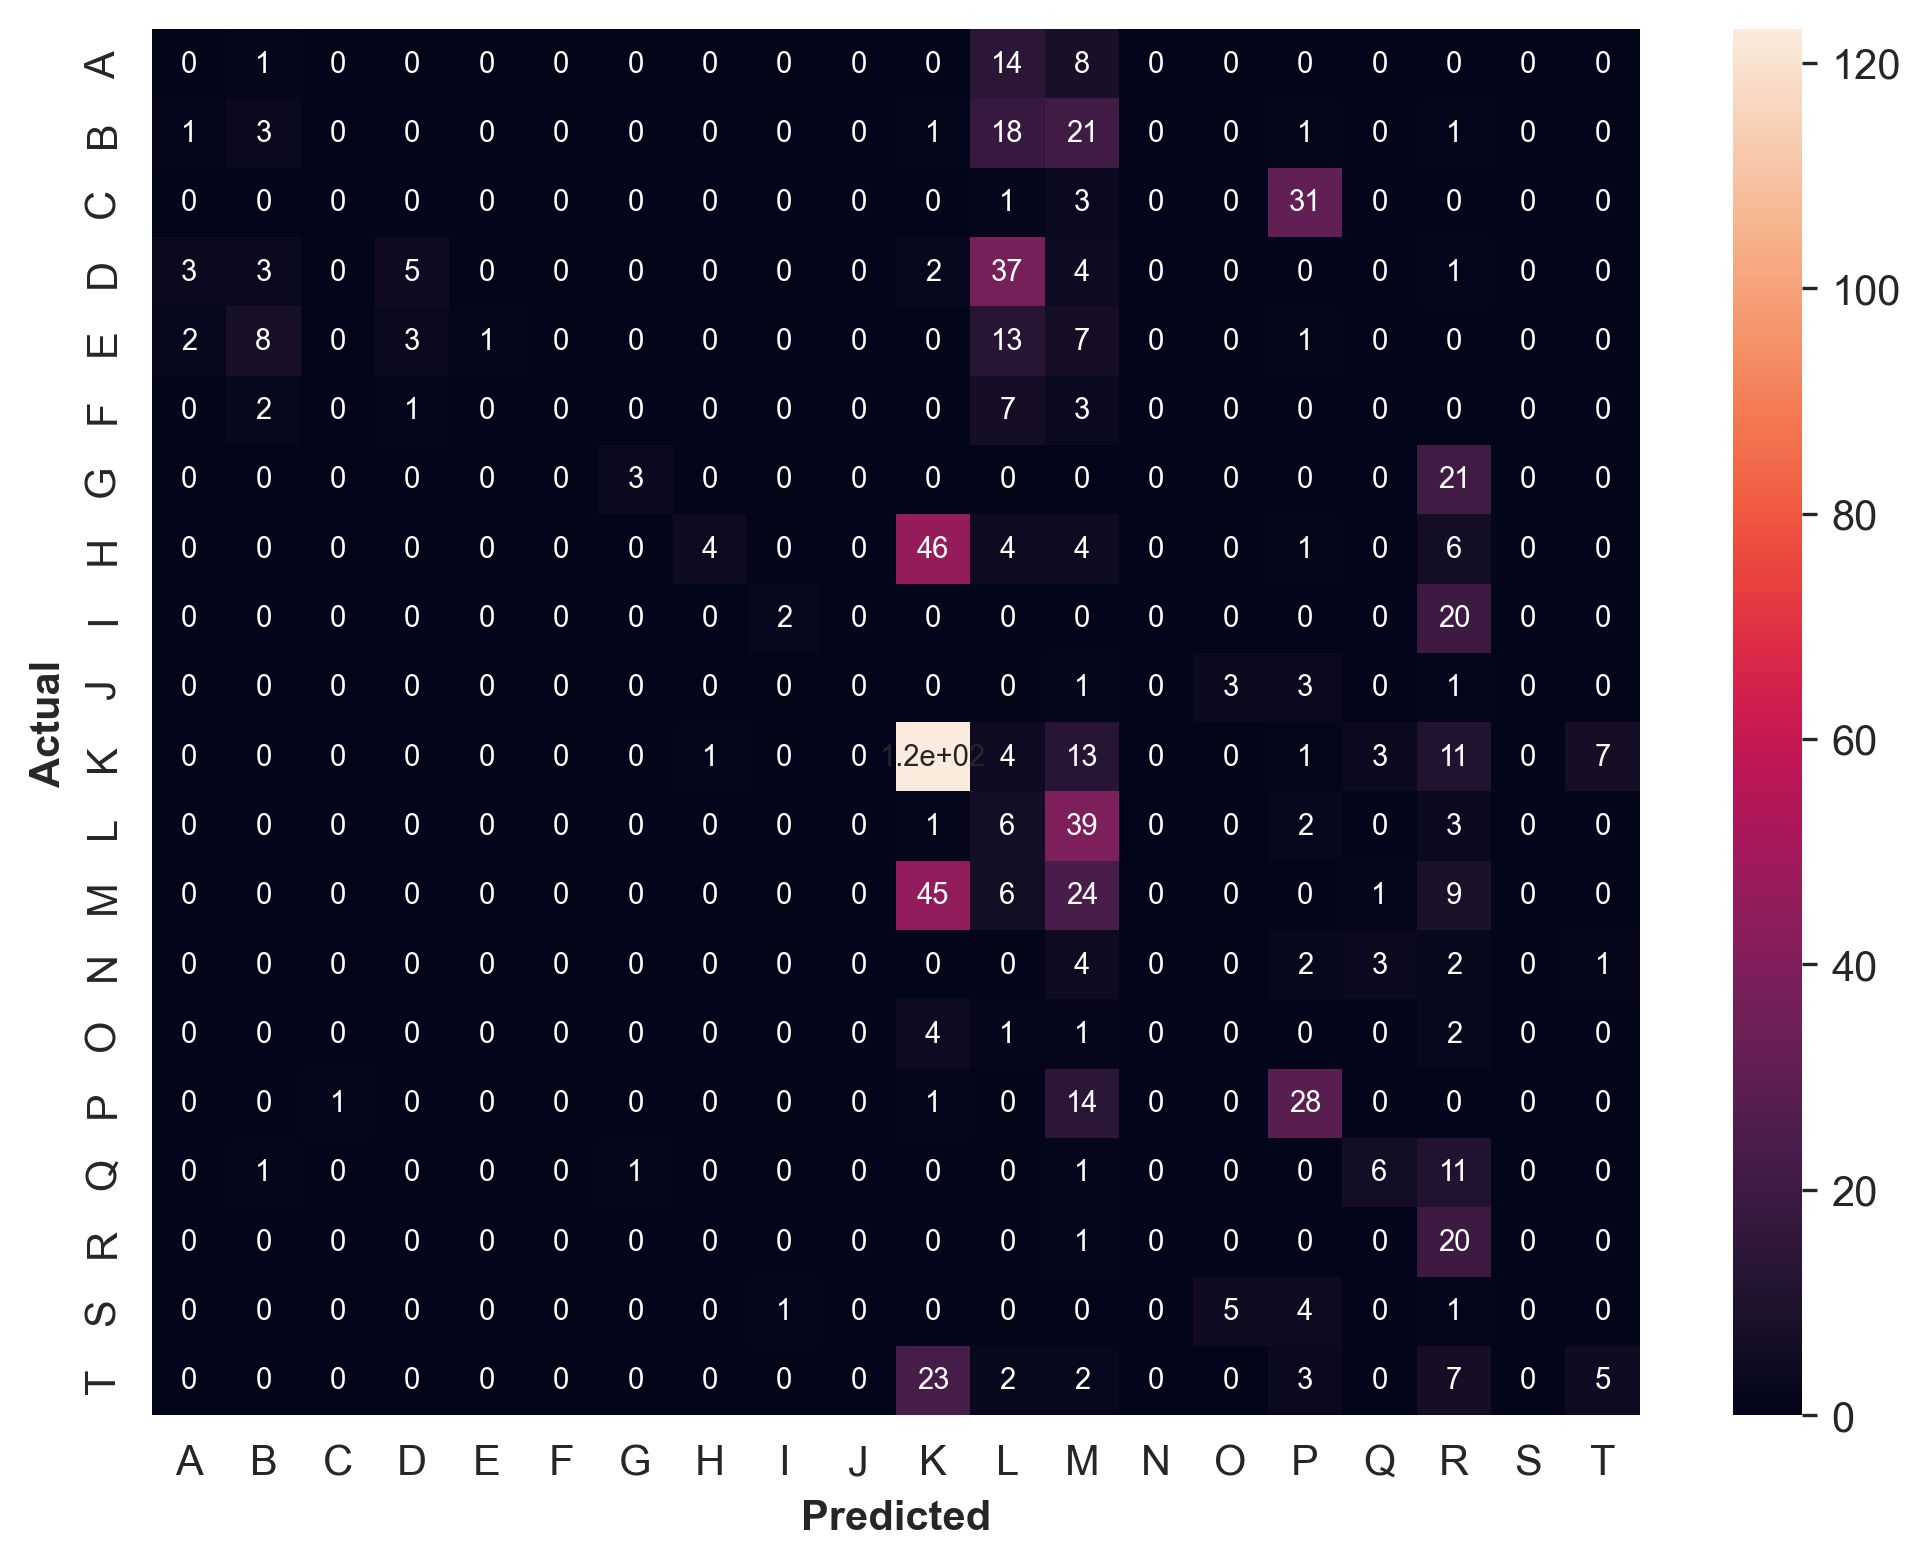
\includegraphics[width=\textwidth]
        {figures/experiment1-conf-matrix-mobilenet_v3_small.png}
        \caption{\texttt{mobilenet\_v3\_small}}
    \end{subfigure}%
    \begin{subfigure}{.33\textwidth}
        \centering
        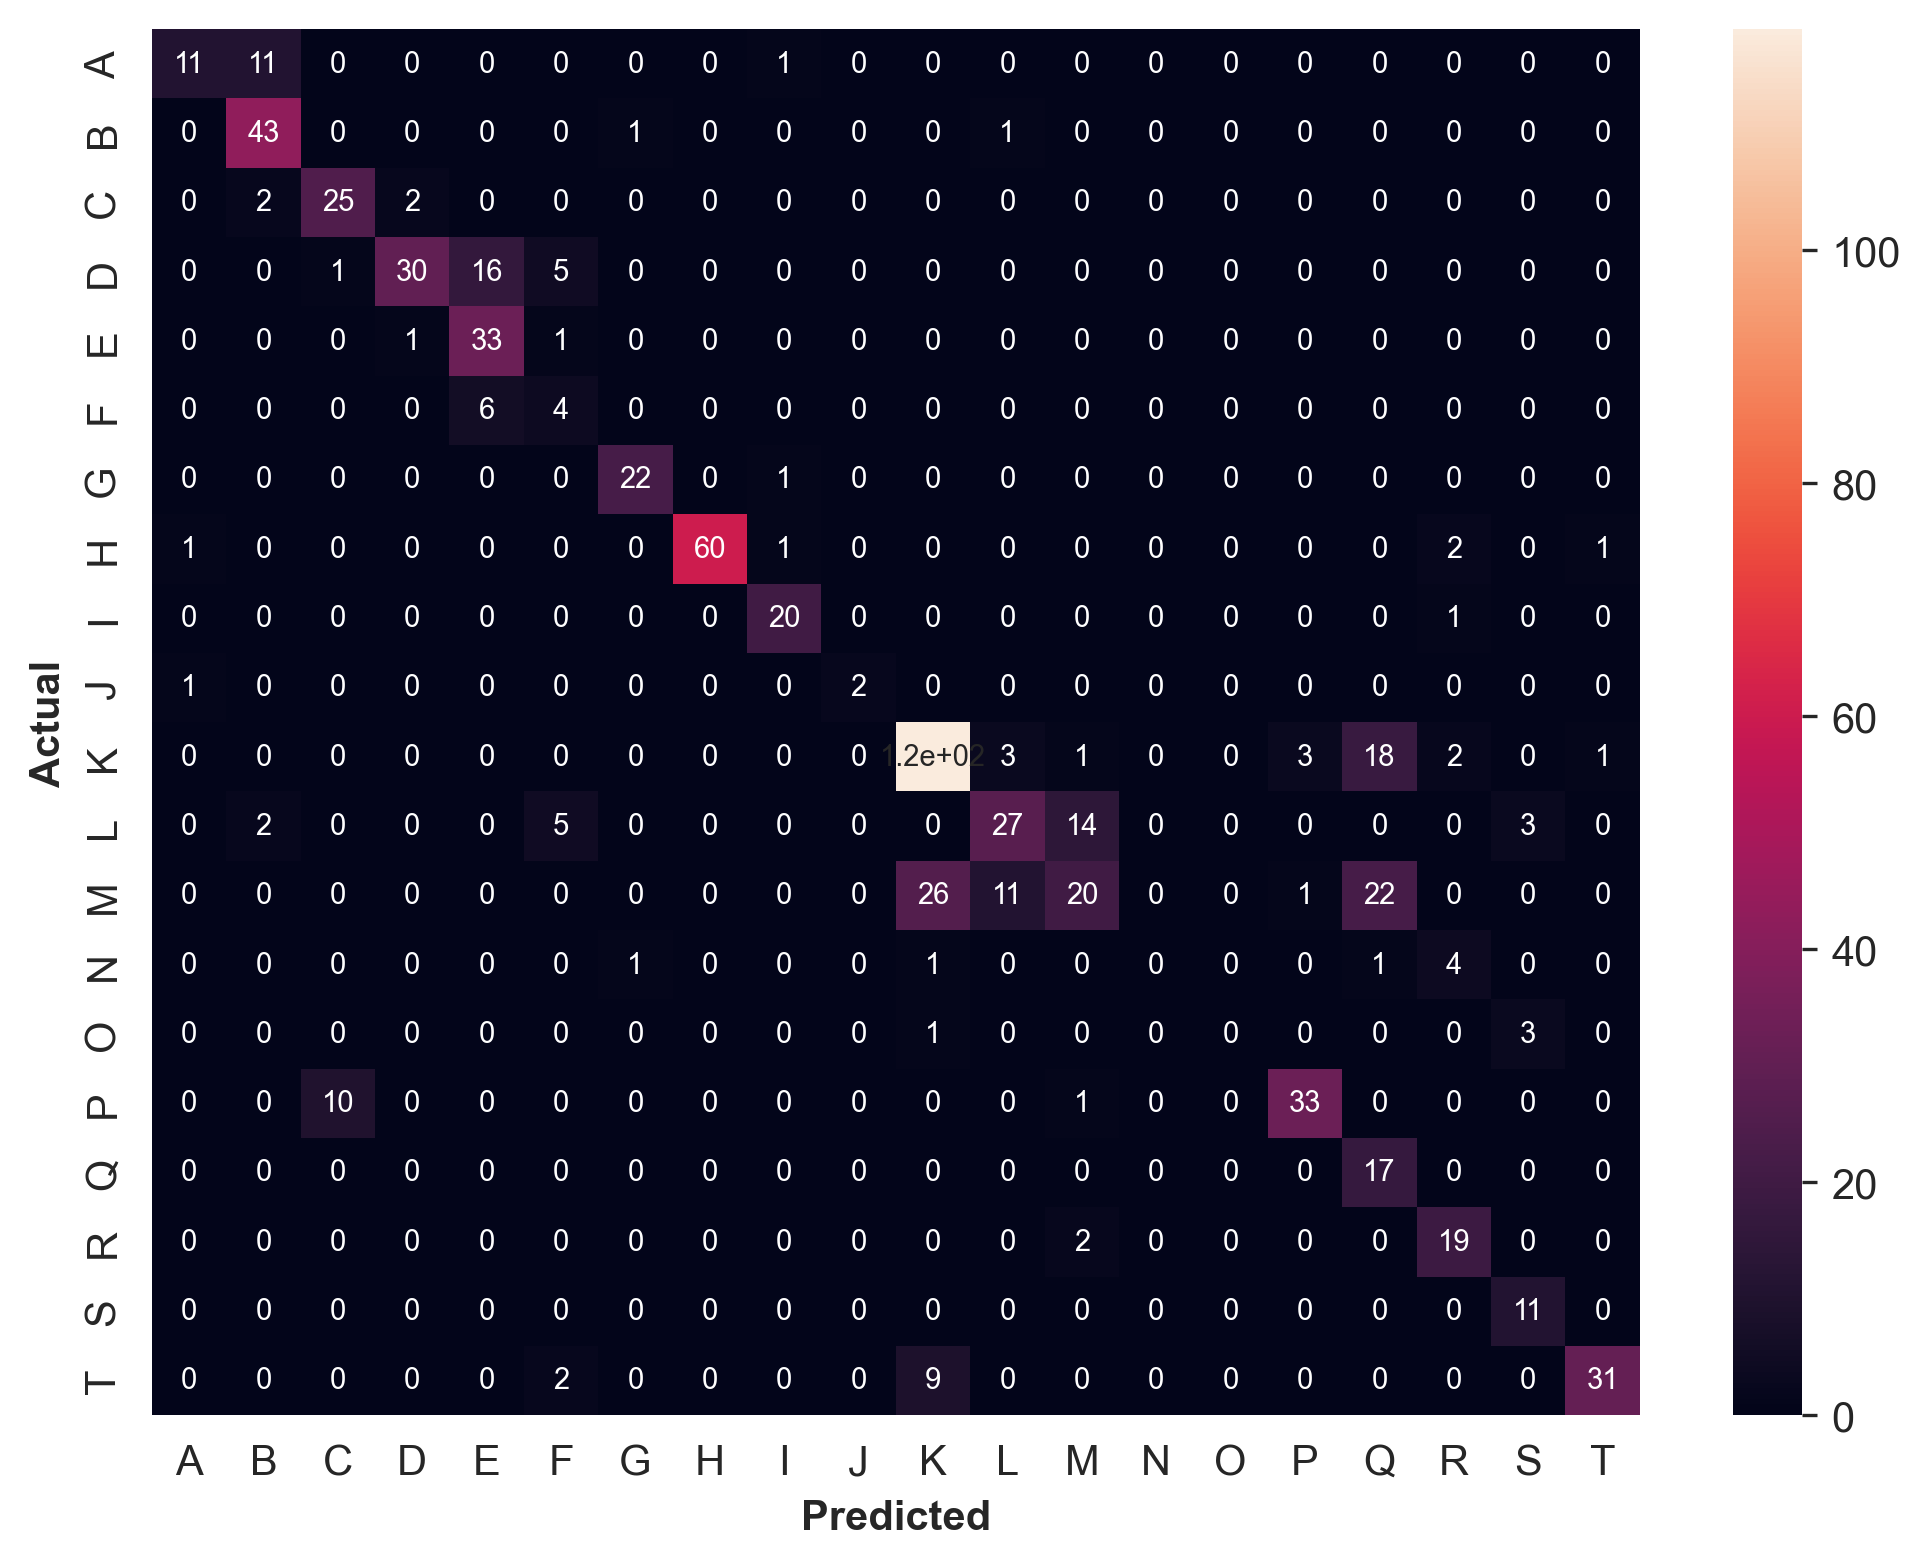
\includegraphics[width=\textwidth]
        {figures/experiment1-conf-matrix-resnet18-lstm.png}
        \caption{\texttt{resnet18-lstm}}
    \end{subfigure}%

    \caption{
      \textbf{Confusion Matrices.} The table shows the (unnormalised) confusion
      matrices of all models in Experiment 1. The predictions are computed on
      the frames from the test split and the matrix. The entry at index $(i,j)$
      is the number of samples with true class $i$ that were predicted to be
      class $j$.
    }

    \label{fig:conf-matrices-experiment1}
  \end{figure}

  \newpage
  \restoregeometry

  % figure
  \begin{figure}[ht]
    \centering
    % subfigure
    \begin{subfigure}[b]{0.49\linewidth}
      \centering
      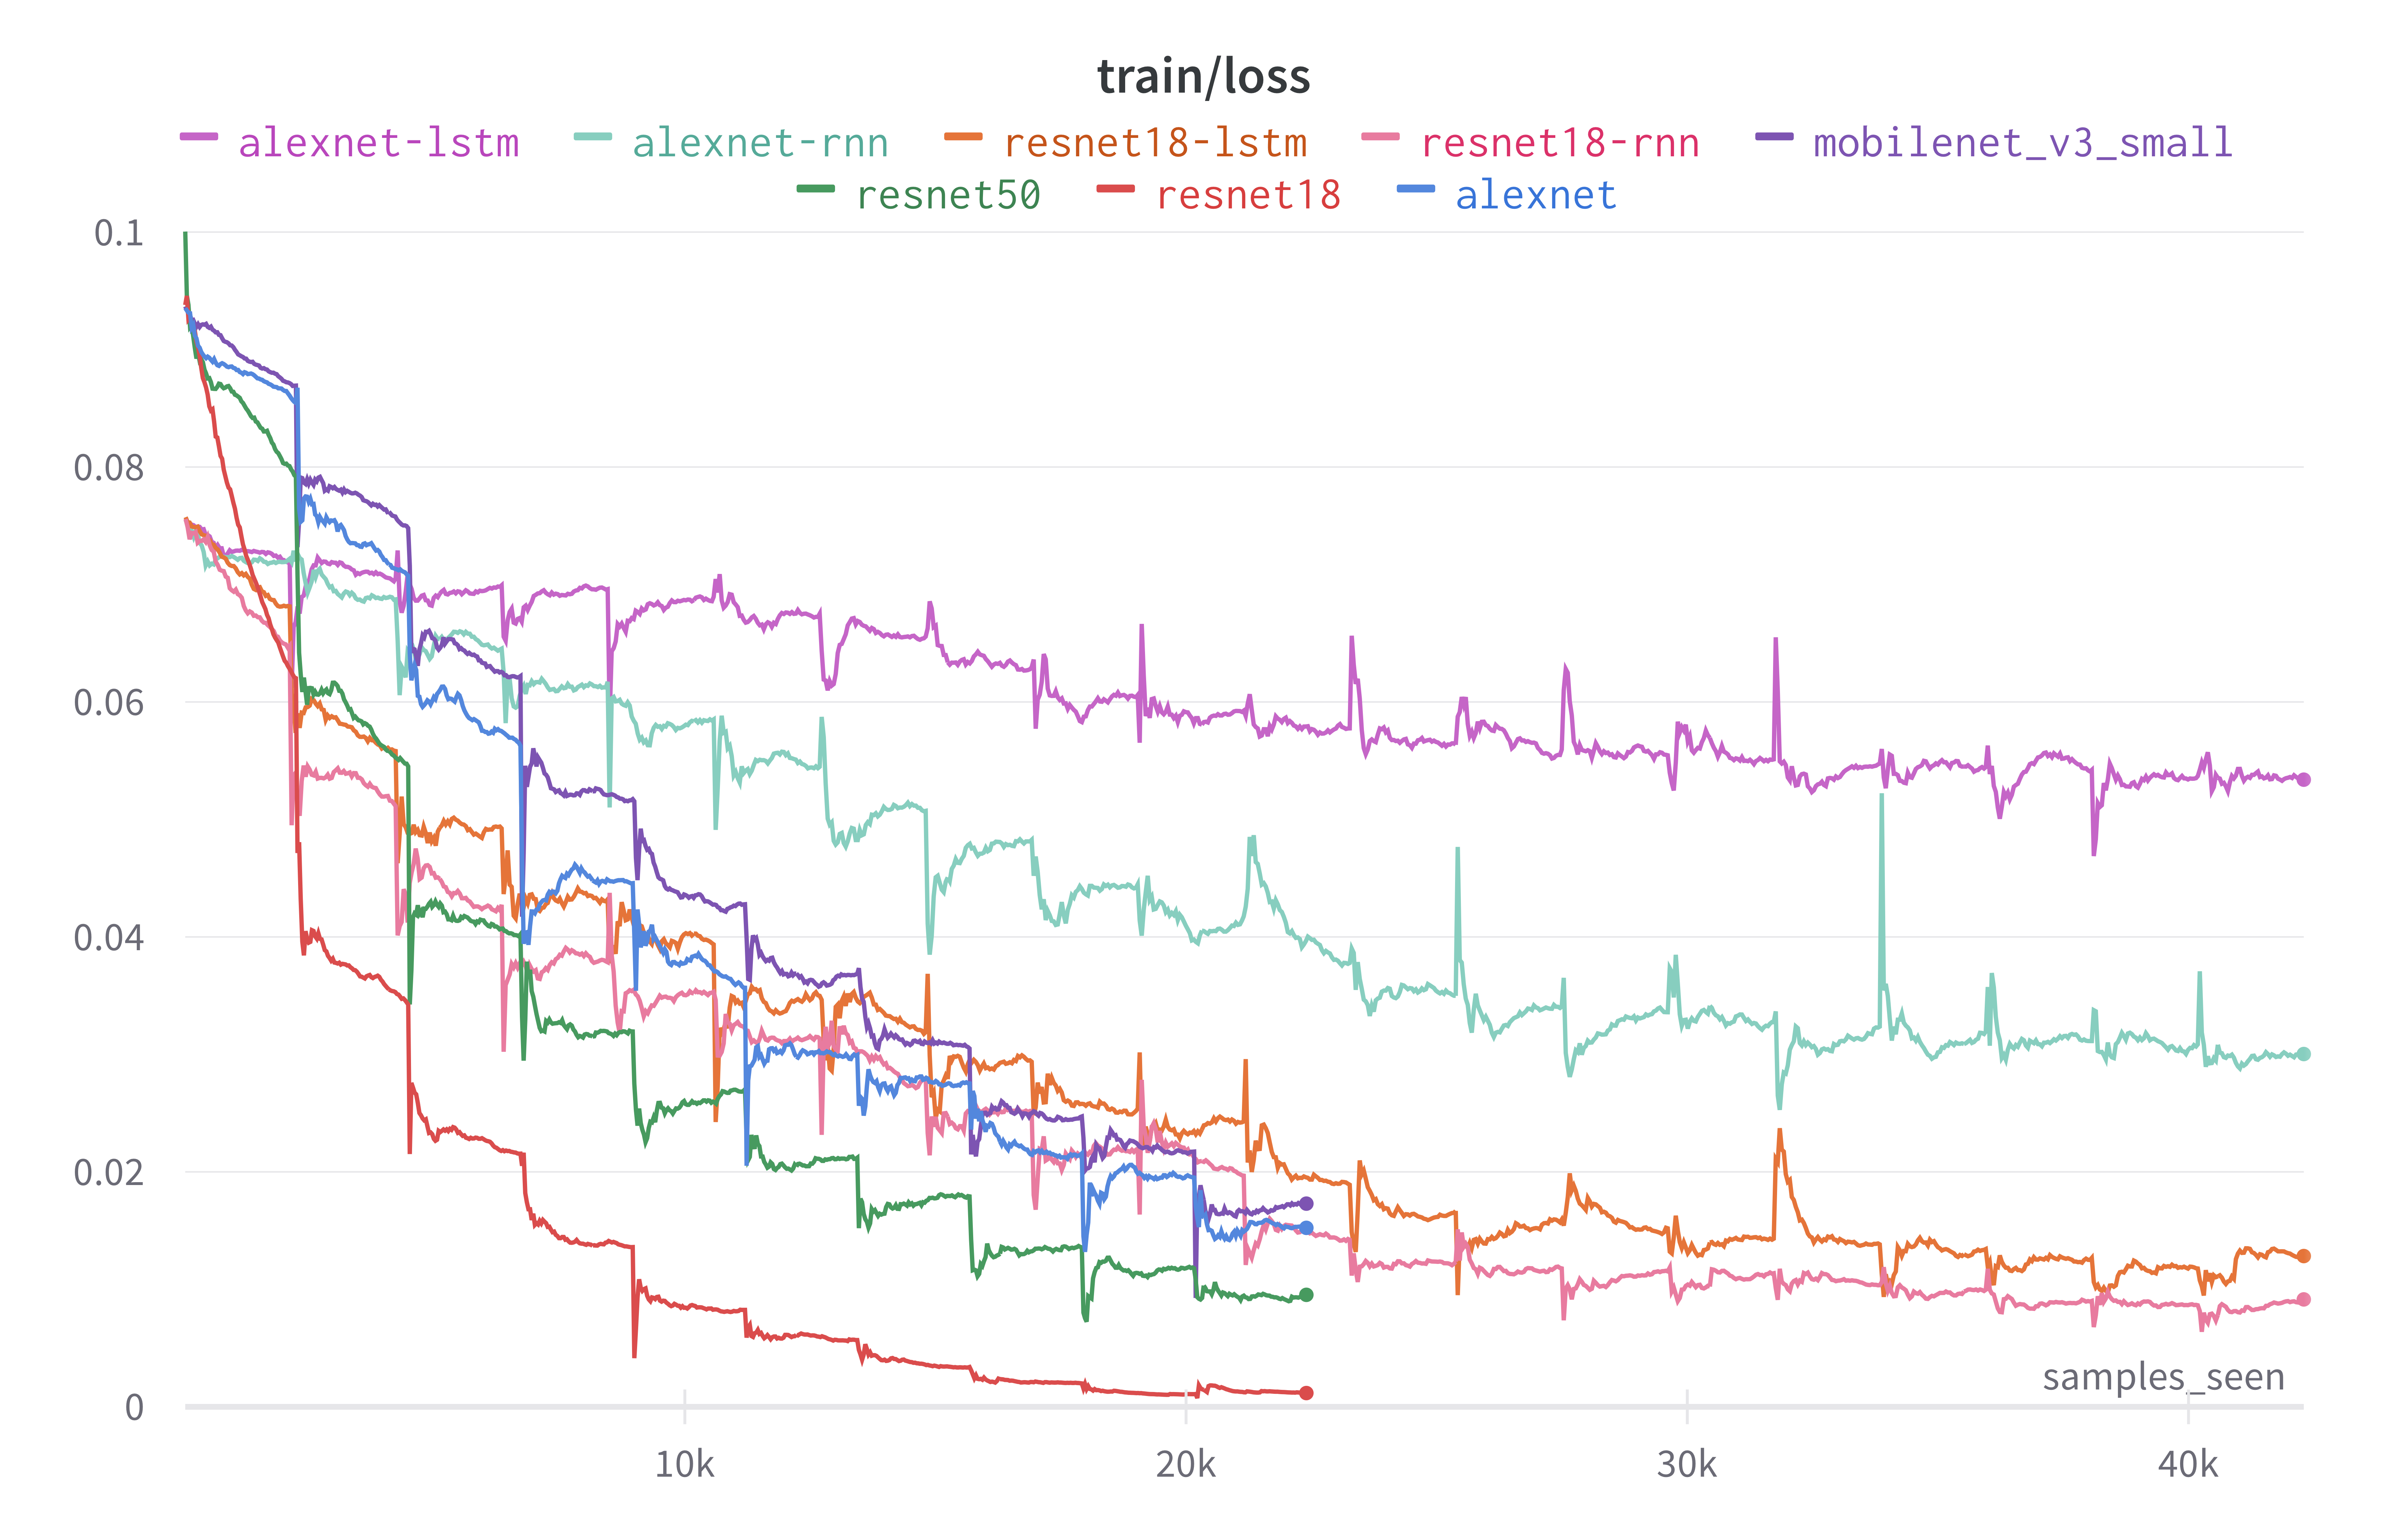
\includegraphics[width=\linewidth]{figures/experiment1-train-loss.png}
      \caption{Training Loss/ Samples}
      \label{fig:experiment1-train-acc}
    \end{subfigure}
    \hfill
    % subfigure
    \begin{subfigure}[b]{0.49\linewidth}
      \centering
      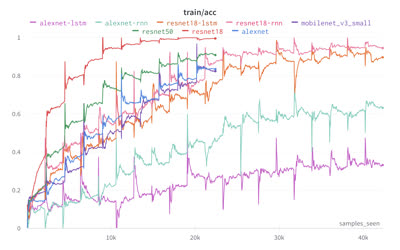
\includegraphics[width=\linewidth]{figures/experiment1-train-acc.jpg}
      \caption{Training Accuracy/ Samples}
      \label{fig:experiment1-train-loss}
    \end{subfigure}
    \caption{Training Metrics for Experiment 1}
    \label{fig:experiment-1-training}
  \end{figure}

  % encoding 
  \begin{table}[ht]
    \centering
    \begin{tabular}{lc}
    \toprule
    \bfseries Class & \bfseries Encoding \\
    \midrule
    First\_Floor\_Corridor\_1 & A \\
    First\_Floor\_Corridor\_2 & B \\
    First\_Floor\_Green\_Area & C \\
    First\_Floor\_Library\_1 & D \\
    First\_Floor\_Library\_2 & E \\
    First\_Floor\_Library\_3 & F \\
    First\_Floor\_Magenta\_Area & G \\
    First\_Floor\_Mezzanine & H \\
    First\_Floor\_Red\_Area & I \\
    First\_Floor\_Yellow\_Area & J \\
    Ground\_Floor\_Atrium & K \\
    Ground\_Floor\_Corridor\_1 & L \\
    Ground\_Floor\_Corridor\_2 & M \\
    Ground\_Floor\_Entrance\_Magenta & N \\
    Ground\_Floor\_Entrance\_Yellow & O \\
    Ground\_Floor\_Green\_Area & P \\
    Ground\_Floor\_Magenta\_Area & Q \\
    Ground\_Floor\_Red\_Area & R \\
    Ground\_Floor\_Yellow\_Area & S \\
    Stairs\_Atrium & T \\
    \bottomrule
    \end{tabular}
    \caption{Encoding of Classes}
    \label{tab:class-encoding}
  \end{table}

  % figure
  \begin{figure}[ht]
    \centering
    % subfigure
    \begin{subfigure}[b]{0.49\linewidth}
      \centering
      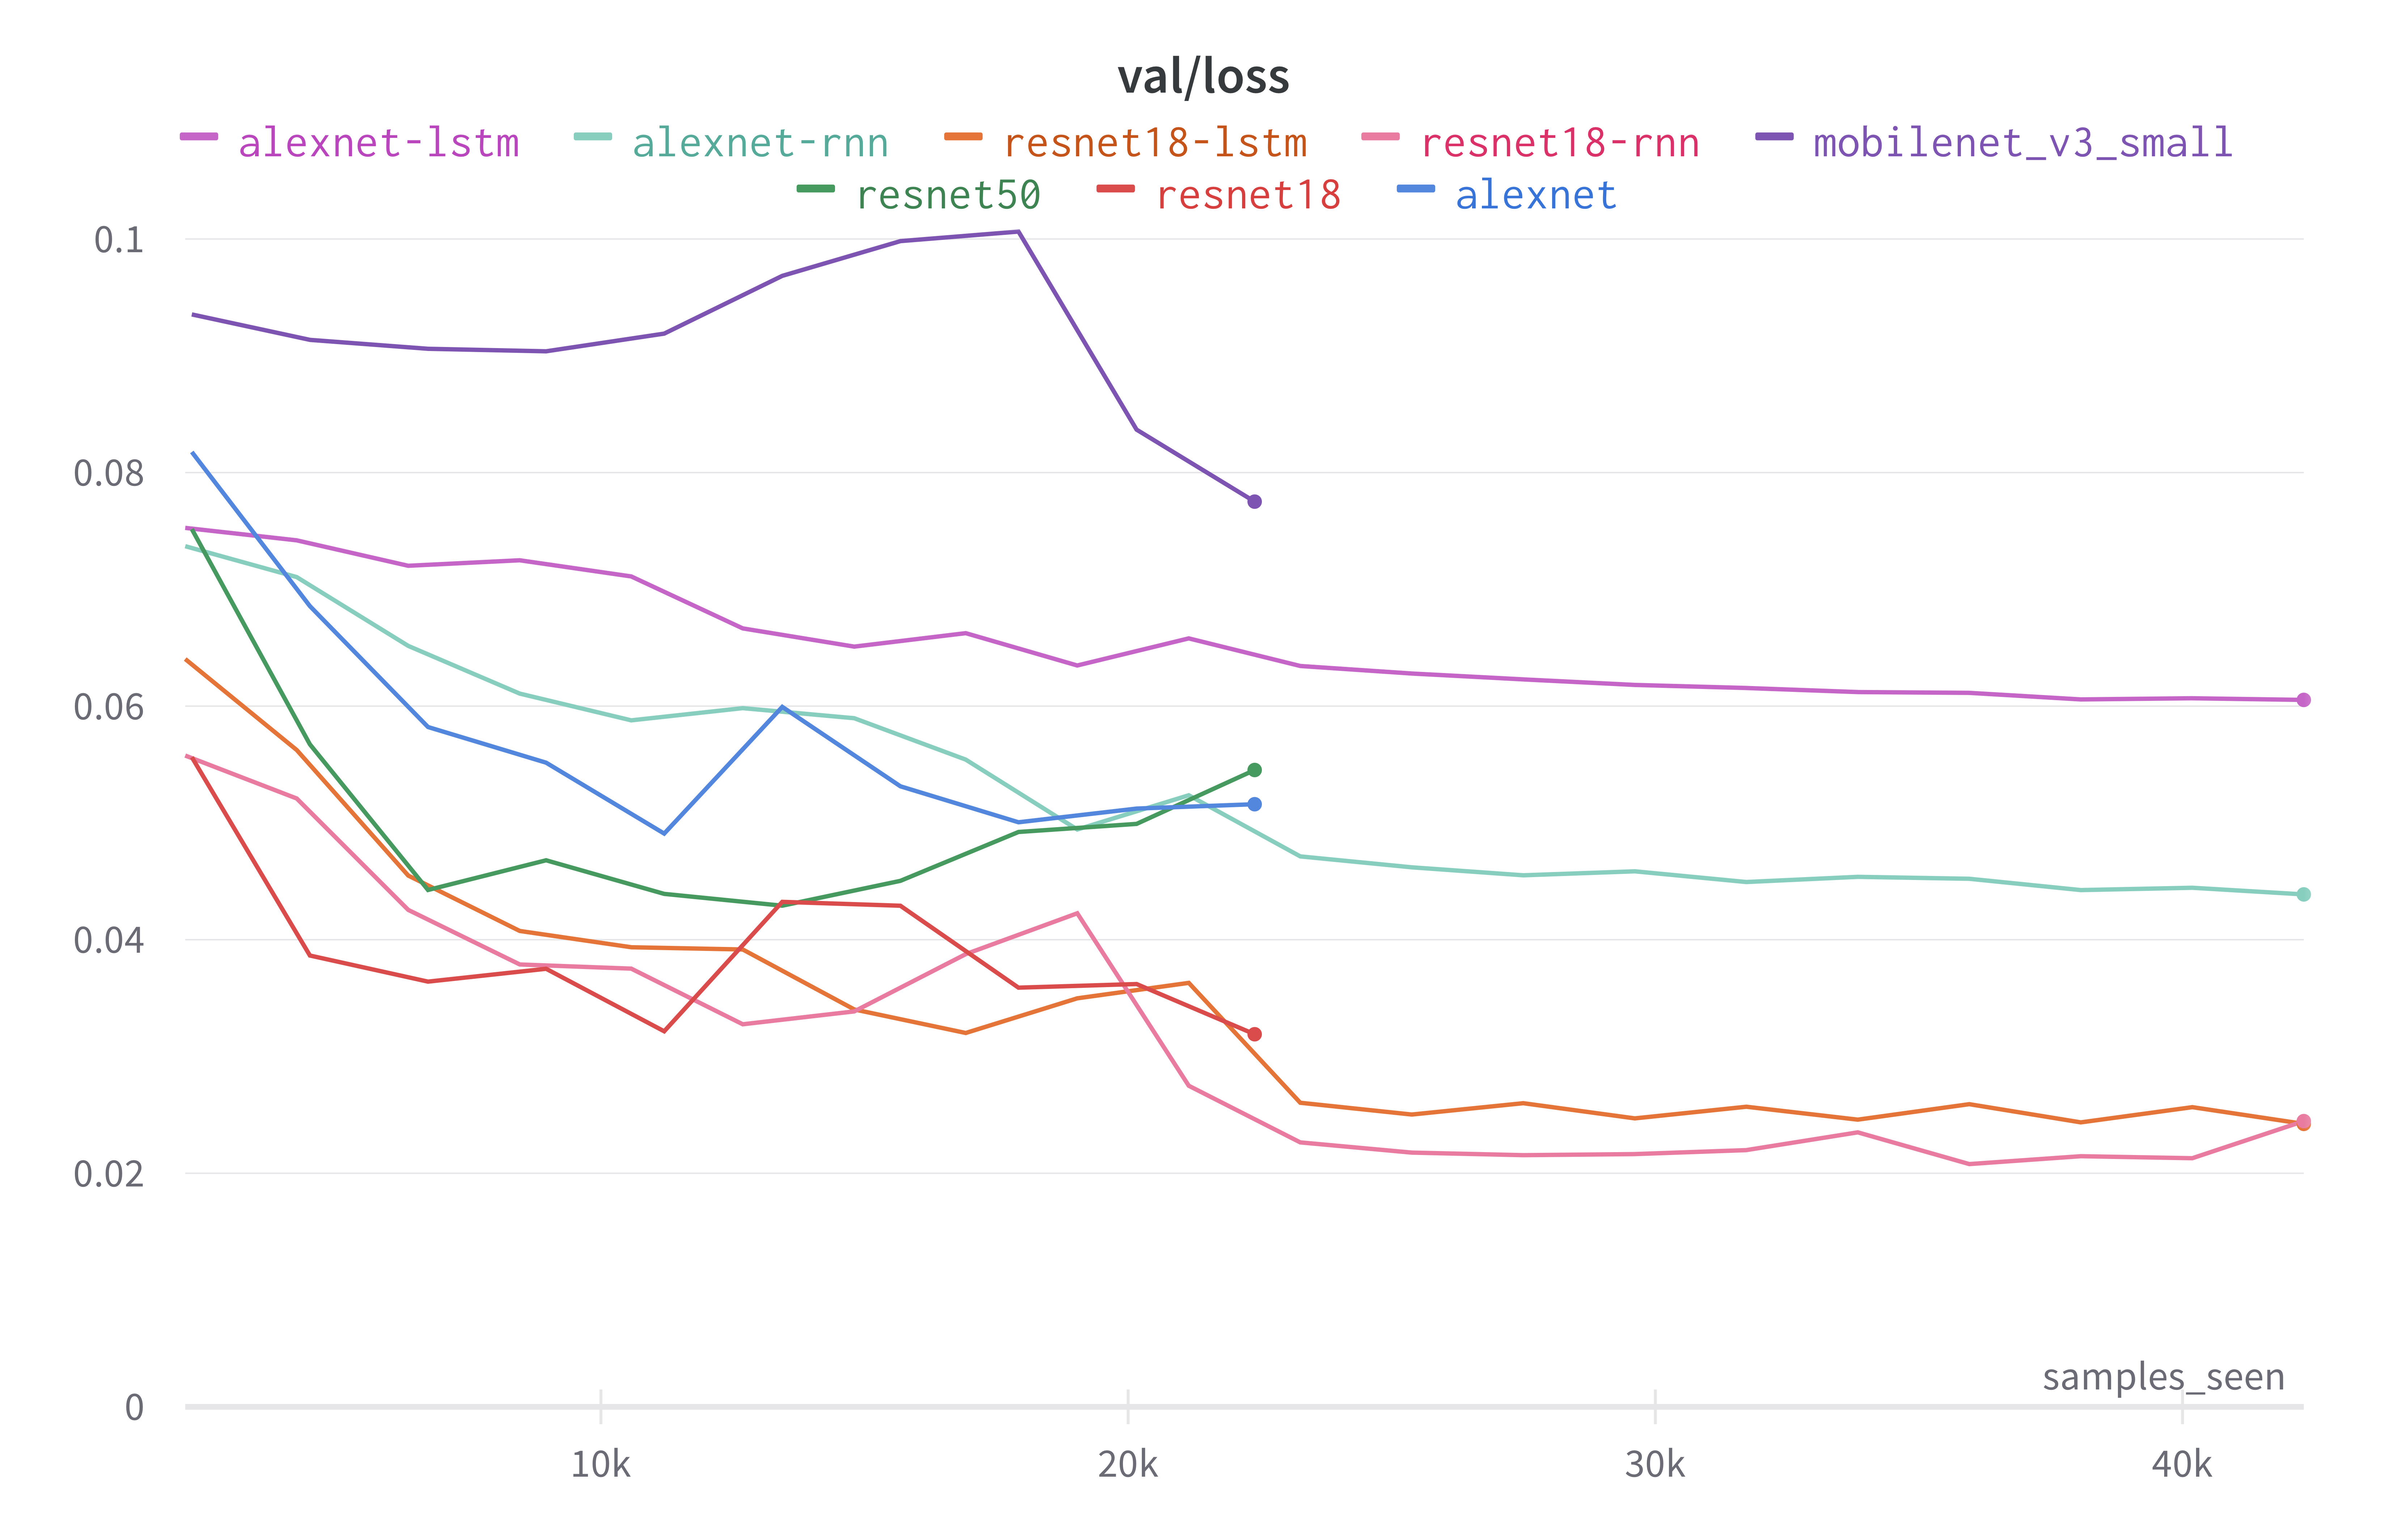
\includegraphics[width=\linewidth]{figures/experiment1-val-loss.png}
      \caption{Validation Loss/ Samples}
      \label{fig:experiment1-val-acc}
    \end{subfigure}
    \hfill
    % subfigure
    \begin{subfigure}[b]{0.49\linewidth}
      \centering
      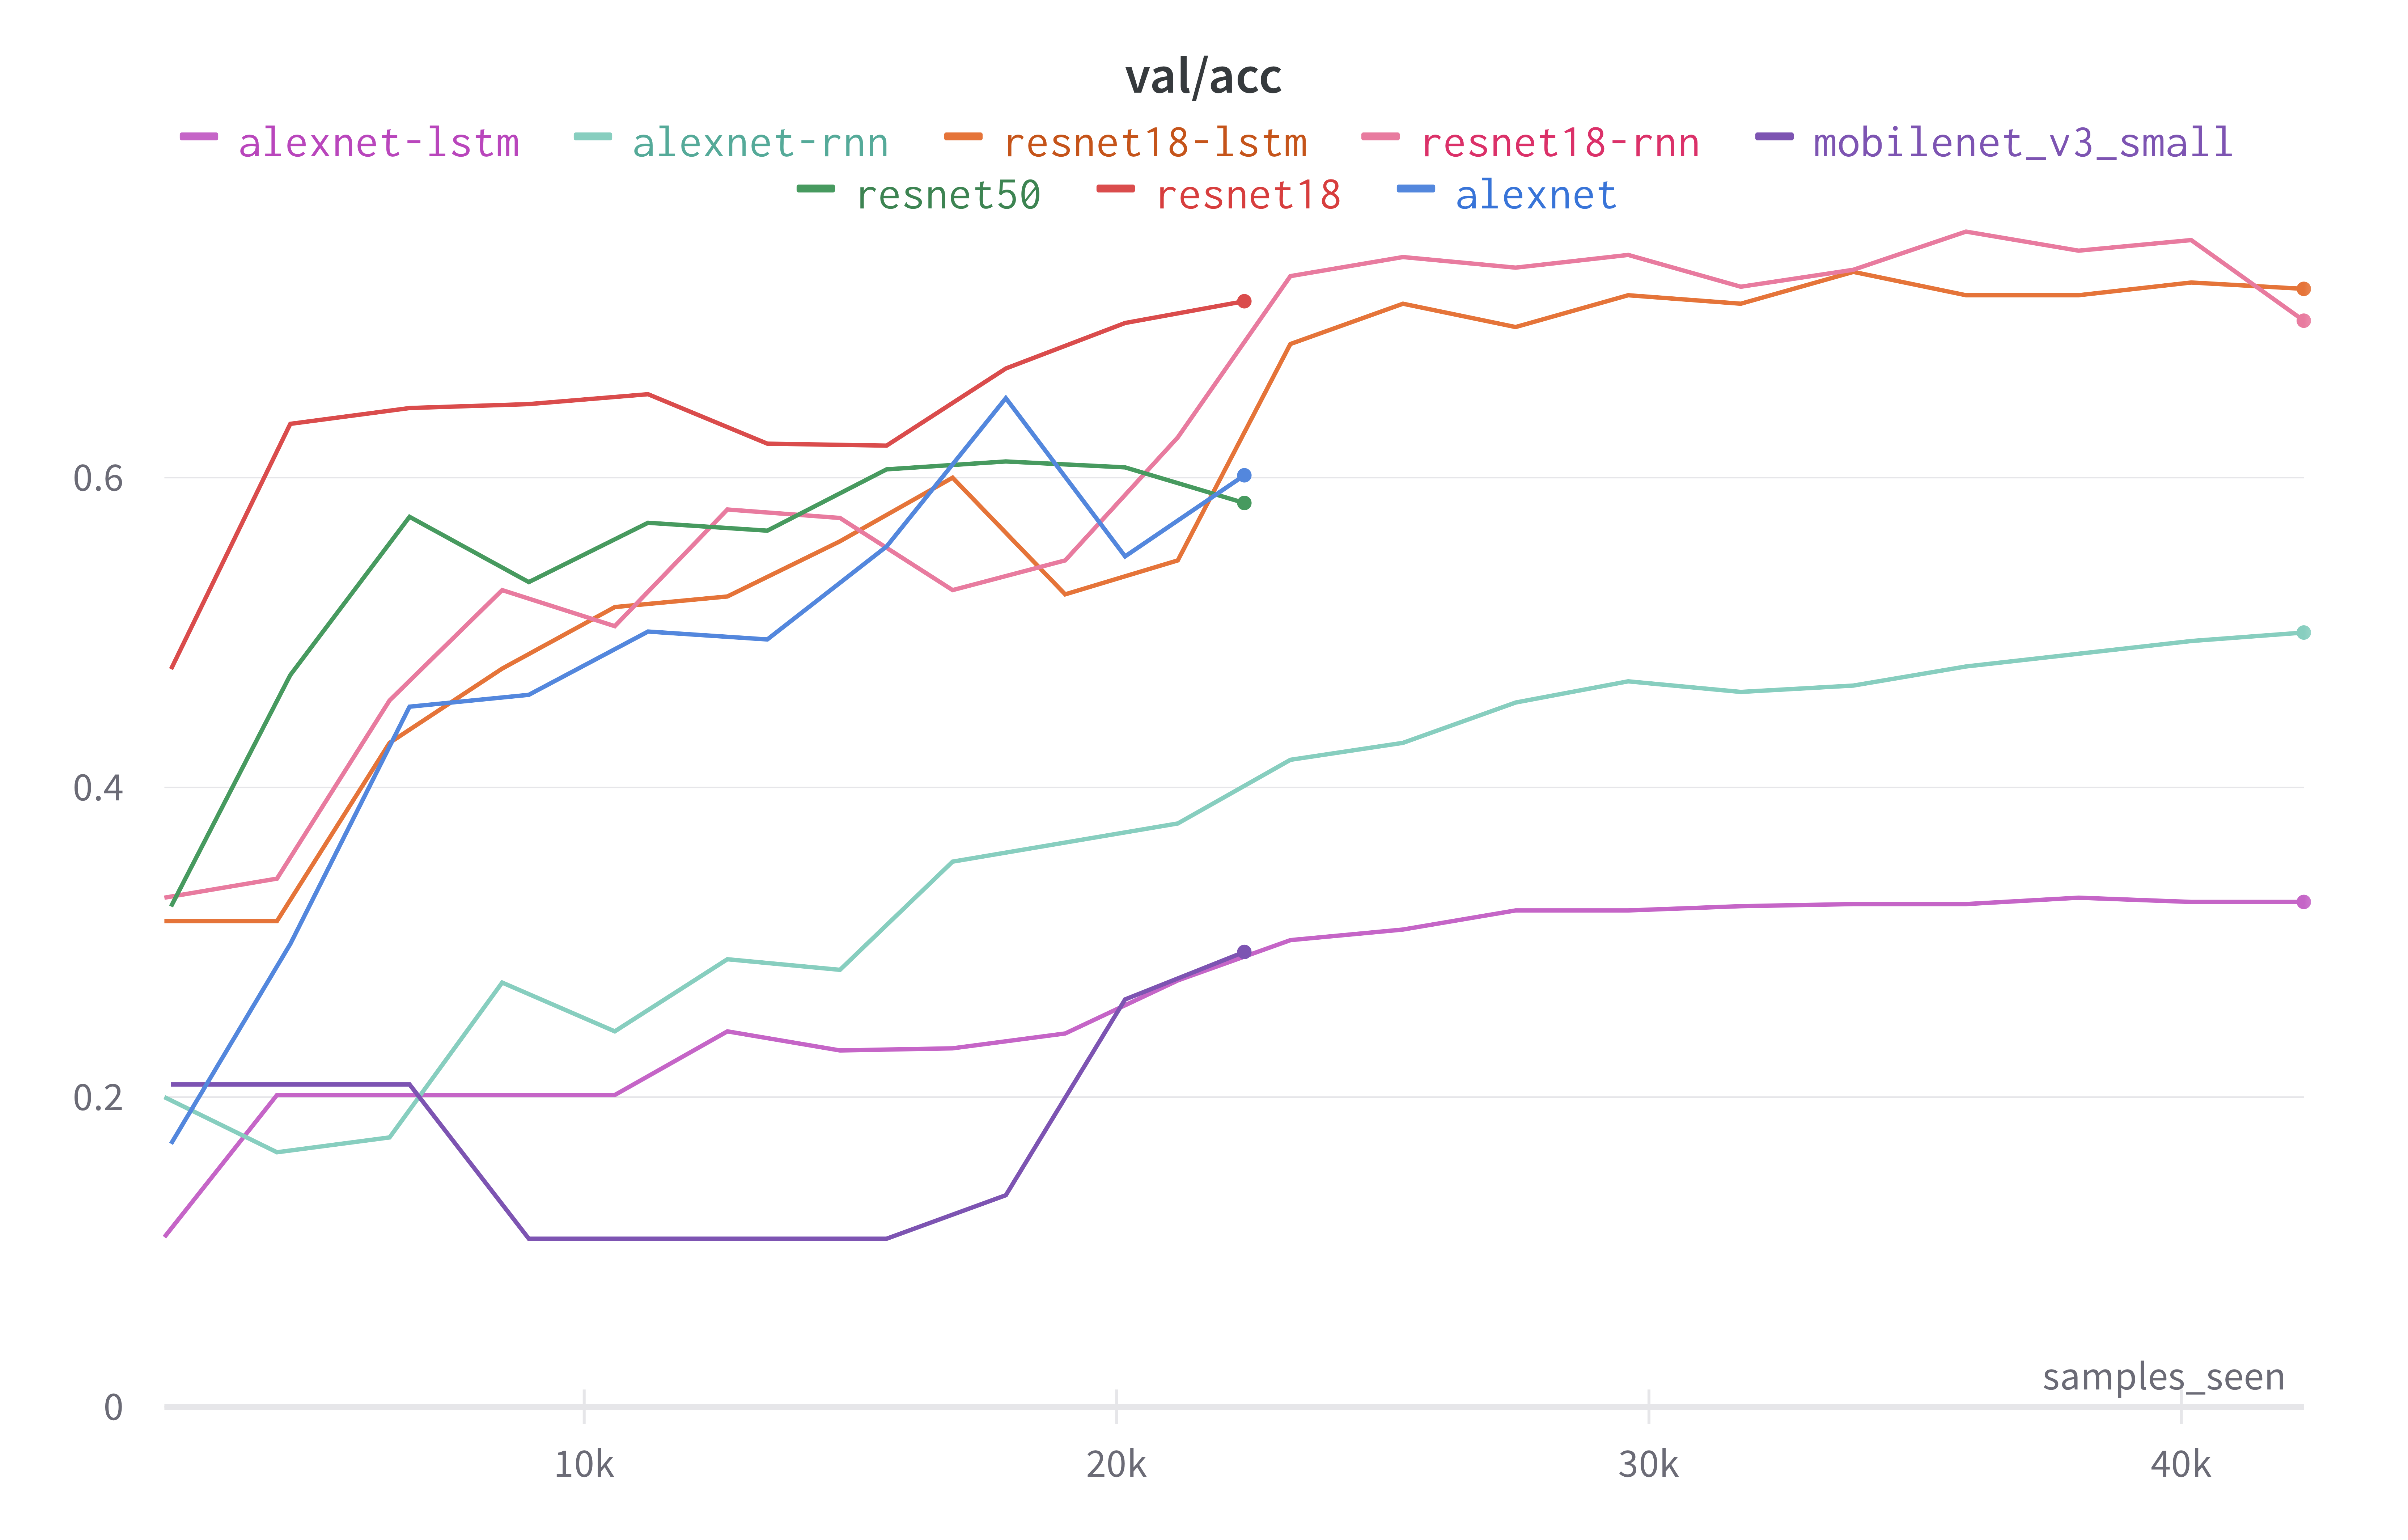
\includegraphics[width=\linewidth]{figures/experiment1-val-acc.png}
      \caption{Valiation Accuracy/ Samples}
      \label{fig:experiment1-val-loss}
    \end{subfigure}
    \caption{Validation Metrics for Experiment 1}
    \label{fig:experiment-1-validation}
  \end{figure}

  % section appendix (end)
  

\end{document}
